\documentclass{report}
\usepackage[margin=2cm]{geometry}
\usepackage{amsmath}
\usepackage{chemformula}
\usepackage[title,titletoc]{appendix}
\usepackage[final]{pdfpages}
\usepackage{titlesec}
\usepackage{hyperref}
\usepackage{cite}

\usepackage{caption}
\captionsetup{font=small,labelfont=bf,margin={1cm,1cm}}

\newtheorem{question}{Question}
\newtheorem{definition}{Definition}


% Opponents: Beatriz Roldan Cuenya and Aliaksandr Bandarenka


\newcommand\Tstrut{\rule{0pt}{3ex}}         % = `top' strut
\newcommand\Bstrut{\rule[-1.2ex]{0pt}{0pt}}   % = `bottom' strut

\begin{document}

\pagenumbering{roman}

%
\begin{titlepage}



\begin{center}
\parindent=0pt
\flushleft

\newcommand{\HRule}{\rule{\textwidth}{1mm}}

\Large{\textbf{Ph.D. Thesis}}

%\vspace*{1cm}
\HRule

\vspace{3mm}
\LARGE{\textbf{Isotope-Labeling Studies in Electrocatalysis}}\\

\vspace{3mm}
\large{\textit{\textbf{And the net \ch{CO2} impact of this PhD Project}}}


\end{center}

\vfill

\begin{figure}[h!]
	\begin{center}
	\advance\leftskip-1cm
	\includegraphics[width=1\textwidth]{Decor/fig/coverfig.png}	
	\end{center}
\end{figure}

\vfill
\noindent
\parindent=0pt
\Large{\textbf{Soren Bertelsen Scott}}

\vspace{5mm}

Supervisor: Professor Ib Chorkendorff

Technical University of Denmark

Department of Physics

Surface Physics and Catalysis (SurfCat)

Villum Center for the Science of Sustainable Fuels and Chemicals

\vspace{5mm}

August 2019
\end{titlepage}
%\section*{Abstract}


%\section*{Foreword}

\subsection*{This project}


\subsection*{This thesis}

As the months and weeks remaining in my PhD project grew more and more limited, I began to ask myself what I wanted to do with my PhD Thesis. Two answers to that question surfaced, which I have tried to accomplish:
\begin{itemize}
	\item I wanted to get down the scientific ideas that I've had during this PhD project that aren't in articles, especially those that might not ever get into articles.

	\item I wanted to write a PhD thesis that others would find useful and read in the future. 
\end{itemize}


\subsection*{Acknowledgements}


%\chapter*{List of Papers}

%\subsection*{Notes}
The Chapters of this Thesis do not seek to repeat or summarize any of the papers I have been involved in, but instead to tell an independent story which sometimes comments and expands on the papers. Furthermore, while the Thesis does not cover all of what I've done during my PhD, it would not make complete sense to choose some of the papers to call within the scope of the thesis and leave the others out. All of the papers contributed to my thinking during this PhD project, and all are mentioned in the Chapters of the Thesis, if only in passing. They are therefore all included here indiscriminately, in order of publication or expected publication. Nonetheless, some are of course more central than others. Chapter \ref{ch:Tools} comments and expands on Paper \ref{Trimarco2018}, and takes inspiration from work done behind the scenes of Paper \ref{Winiwarter2019}. Chapter \ref{ch:O2} includes and comments on some of the most important results of Paper \ref{Roy2018} and includes most of the content of what we expect to publish as Paper \ref{Scott_Rao2019}. 

Paper \ref{Nitopi2019} is notable among them for being a review and perspective article. My most important contribution to this work was writing the introduction, which includes an outline of the anthropogenic contribution to the global carbon cycle and strategies to close it. While in Paper \ref{Nitopi2019}, this outline is used to motivate the direct electrocatalytic reduction of \ch{CO2}, it also motivates improving the efficiency and cost-effectiveness of hydrogen production via water splitting. Because Paper \ref{Nitopi2019} is very long, I have only included the introduction in this thesis.

Here is the full list:
\vspace{10mm}
%\parindent=0pt
\begin{flushleft}


\noindent\textbf{Paper \ref{Trimarco2018}} \hfill page~\pageref{Trimarco2018}

\textbf{Enabling Real-Time Detection of Electrochemical Desorption Phenomena with Sub-Monolayer Sensitivity} 

		\underline{Soren B. Scott}*, Daniel B. Trimarco*, Anil H. Thilsted, Jesper Y. Pan, Thomas Pedersen, Ole Hansen, Ib Chorkendorff, and Peter C.K. Vesborg. 
		
		*These authors contributed equally to this work
		
		\textit{Electrochimica Acta}, 2018, 268, 520-530
		
		DOI: 10.1016/j.electacta.2018.02.060
		
		


\vspace{5mm}
\noindent\textbf{Paper \ref{Roy2018}}  \hfill page~\pageref{Roy2018}

\textbf{Impact of nanoparticle size and lattice oxygen on water oxidation on \ch{NiFeO$_x$H$_y$}} 

	\underline{Soren B. Scott}*, Claudie Roy*, Bela Sebok*, Elisabetta M. Fiordaliso, Jakob E. Sørensen, Anders Bodin, Daniel B. Trimarco, Christian D. Damsgaard, Peter C. K. Vesborg, Ole Hansen, Ifan E. L. Stephens, Jakob Kibsgaard and Ib Chorkendorff. 

	*These authors contributed equally to this work
	
	\textit{Nature Catalysis}, 2018, 1(11), 820-829 
	
	DOI: 10.1038/s41929-018-0162-x



\vspace{5mm}
\noindent\textbf{Paper \ref{Winiwarter2019}}  \hfill page~\pageref{Winiwarter2019}

\textbf{Towards an Atomistic Understanding of Electrocatalytic Partial Hydrocarbon Oxidation: Propene on Palladium} 

Anna Winiwarter*, Luca Silva*, \underline{Soren B. Scott}, Kasper Enemark-Rasmussen, Manuel Saric, Daniel B. Trimarco, Peter C. K. Vesborg, Poul G. Moses, Ifan E. L. Stephens, Brian Seger, Jan Rossmeisl, and Ib Chorkendorff.

*These authors contributed equally to this work

\textit{Energy and Environmental Science}, 12, 1055-1067, 2019.

DOI:  10.1039/C8EE03426E


\vspace{5mm}
\noindent\textbf{Paper \ref{Scott2019_GIXRD}} \hfill page~\pageref{Scott2019_GIXRD}

\textbf{Absence of Oxidized Phases in Cu under CO Reduction Conditions} 

\underline{Soren B. Scott}, Thomas V. Hogg, Alan T. Landers, Thomas Maagaard, Erlend Bertheussen, John C. Lin, Ryan C. Davis, Jefferey W. Beeman, Drew Higgins, Walter S. Drisdell, Apurva Mehta, Brian J. Seger, Thomas F. Jaramillo, and Ib Chorkendorff.

\textit{ACS Energy Letters}. 4, 803−804, 2019

DOI: 10.1021/acsenergylett.9b00172


\vspace{5mm}
\noindent\textbf{Paper \ref{Nitopi2019}} \hfill page~\pageref{Nitopi2019}

\textbf{Progress and Perspectives of Electrochemical CO2 Reduction on Copper in Aqueous Electrolyte} 

Stephanie A. Nitopi*, Erlend Bertheussen*, \underline{Soren B. Scott}, Xinyan Liu, Albert K. Engstfeld, Sebastian Horch, Brian Seger, Ifan Stephens, Karen Chan, Christopher Hahn, Jens K. Nørskov, Thomas Jaramillo, and Ib Chorkendorff.

*These authors contributed equally to this work

\textit{Chemical Reviews}. 12, 7610-7672, 2019

DOI: 10.1021/acs.chemrev.8b00705



\vspace{5mm}

\noindent\textbf{Paper \ref{Scott_Engstfeld2019}} \hfill page~\pageref{Scott_Engstfeld2019}
	
\textbf{Desorbing uphill: Anodic Hydrogen Evolution on Cu and Ru Electrodes} 

\underline{Søren B. Scott}*, Albert K. Engstfeld*, Zenonas Yusys, Degenhart Hochfilzer, Nikolaj Knøsgaard, Daniel B. Trimarco, Peter C.K. Vesborg, R. Jürgen Behm, and Ib Chorkendorff

*These authors contributed equally to this work

\textit{In Preparation}


\vspace{5mm}
\noindent\textbf{Paper \ref{Scott_Rao2019}} \hfill page~\pageref{Scott_Rao2019}

\textbf{Mechanistic study of oxygen evolution on \ch{RuO2} down to 60 mV overpotential}

\underline{Soren B. Scott}*, Reshma R. Rao*, Choongman M. Moon, Jakob E. S\o rensen, Jakob Kibsgaard, Yang Shao-Horn, and Ib Chorkendorff

*These authors contributed equally to this work

\textit{In Preparation}



\end{flushleft}

\setcounter{tocdepth}{2}
\tableofcontents\thispagestyle{empty}\clearpage


\pagenumbering{arabic}
\setcounter{page}{1}

%
\chapter{Introduction: The Climate Crisis}

It was right around the year in which I was born that the American political economist Francis Fukuyama captured the mood of much of the world by claiming that history was ending\cite{Fukuyama1992}. This feeling was based on the fall of the Berlin wall and with it what seemed like the inevitable spread to the entire world of societal structures and lifestyles based on inclusive liberal democracy, technological progress, and market capitalism tempered to varying extent by regulatory welfare states. Now, a widely accepted view that history was ending seems itself to be part of a rather brief moment in history, shattered 
%in part by wars and revolutions that broadly failed in their (generously interpreted) intentions of spreading democracy, the astounding success (in some respects) of China's politically authoritarian societal model, and a growth of illiberal political views in established democracies. 
by several waves of headline-dominating setbacks to the advancement of these supposedly victorious ideals.
But nothing poses a more devastating blow to the supposed inevitability of our lifestyles and societies than does the fact that they are simply unsustainable. History is not over, because if we try to keep on living the way we do today, we won't be able to keep living on this planet.

\begin{figure}[h!]
	\centering
	\includegraphics[width=0.7\textwidth]{01_Intro/fig/carbon_cycle.png}
	\caption{Diagram of Earth's carbon cycle. Red numbers indicate the fluxes and accumulations associated with the anthropogenic perturbation. From ref. \citen{DOE2008}, based on data from ref. \citen{LeQuere2015}}
	\label{fig:carbon_cycle}
\end{figure}

The un-sustainability of humanity in its present state encompasses the crossing of or encroaching on multiple interconnected planetary boundaries\cite{Rockstrom2009}, but none pose a more existentially urgent challenge to human civilization than does climate change. The root of our problem, as we summarize it in the introduction to Paper \ref{Nitopi2019}, is that:

\begin{quotation}
		{\Large``} At the core of biological metabolism is the ability to convert carbon between different oxidation states in order to store and release energy, as well as to synthesize functional molecules. Likewise, the oxidation of carbon is at the center of human civilization's collective “industrial metabolism” consisting of our energy infrastructure and chemical industry. Whereas in biological metabolism, reduction of \ch{CO2} in photosynthesis balances the oxidation of carbon in cellular respiration, carbon reduction is as of yet a missing piece of humanity's industrial metabolism. This imbalance has become a significant perturbation to Earth's natural carbon cycle... The resulting accumulation of the greenhouse gas \ch{CO2} in the atmosphere is the primary	driver of today’s climate change\cite{IPCC2014}. {\Large''}
\end{quotation}

This imbalance is illustrated in Figure \ref{fig:carbon_cycle} (from ref. \citen{DOE2008}) and in Table 1 of Paper \ref{Nitopi2019}. So far, since humans began burning fossil fuels at scale in the 1800's, we have moved approximately 400 gigatons of carbon (GtC) from the ground to the air as carbon dioxide (\ch{CO2}), about half of which has stayed in the atmosphere, increasing the atmospheric \ch{CO2} concentration from less than 300 ppm to more than 400 ppm\cite{IPCC2014, LeQuere2018}. At the writing of this Thesis, the atmospheric \ch{CO2} concentration was 412 ppm and increasing at an annualized rate of about 3 ppm per year\cite{NOAA2019}. 

\begin{figure}[h!]
	\centering
	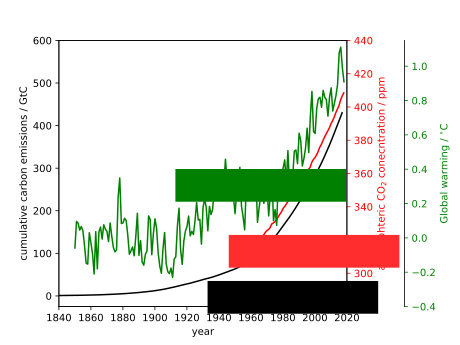
\includegraphics[width=0.7\textwidth]{01_Intro/fig/global_warming.png}
	\caption{Cumulative carbon emissions (black), atmospheric \ch{CO2} concentration (red), and global mean surface temperature relative to the 1850-1900 average (green). Made with data from refs. \citen{LeQuere2018}, \citen{Morice2012}, and \citen{Ritchie2019a}.}
	\label{fig:temperatures}
\end{figure}

Climate science is beyond the scope of this Thesis, but, in brief: \ch{CO2} and other greenhouse gases absorb infrared radiation, unlike the primary components of the atmosphere \ch{N2} and \ch{O2}. Infrared radiation is the main way earth sheds heat to space to balance all the energy coming in as sunlight, so \ch{CO2} in the atmosphere acts like a blanket, heating up the earth. This has so far resulted in an increase in the average temperature of the earth's surface of about 1$^\circ$ C, as shown in Figure \ref{fig:temperatures}. An increase in the average temperature of the earth is worse than it might sound, because the extra energy that this represents effects the entire climate system in profound ways. Climate change is increasing the intensity and frequency of all kinds of extreme weather events including heat waves, forest fires, floods, storms, and droughts\cite{IPCC2014, CarbonBrief}. 
\begin{figure}[h!]
	\centering
	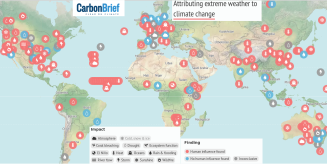
\includegraphics[width=\textwidth]{01_Intro/fig/climate_change_effects.png}
	\caption{Map of extreme weather events from 2011 to 2018. Red indicates that the risk of the extreme weather event was increased by climate change. From %\url{https://www.carbonbrief.org/mapped-how-climate-change-affects-extreme-weather-around-the-world}.
	ref \citen{CarbonBrief}.
}
	\label{fig:attribution}
\end{figure}
Weather is naturally variable, but the science of \textit{climate attribution} has progressed in recent years. Now, the increase in the likelihood due to climate change of a given extreme weather event can be readily calculated, giving a clear picture of the worsening adverse effects of our emissions\cite{Schiermeier2018}. Figure \ref{fig:attribution}, from ref. \citen{CarbonBrief}, shows a map of recent extreme weather events, many of which are attributed to climate change. Extreme weather events and natural disasters are deadly even in developed countries with strong states. In developing countries they can destabilize societies and displace millions\cite{UNHCR2019}. The frequency and severity of climate-change-related extreme weather events will worsen significantly if the present warming trend is not stopped\cite{IPCC2018_SPM}. 

Fortunately for those of us who broadly like living under or aspire to live under enlightenment ideals (and for Fukuyama's assertion), there is still reason to hope that the worst possible outcomes of climate change can be averted within the frameworks of liberal democracy and regulated market capitalism. However, this will not be easy. It will require far-sightedness on the part both of leaders and of everyone who chooses them. It will require almost unprecedented willpower from many corners of society. We will almost certainly need to change our lifestyles significantly, and we will with complete certainty have to change the way we power our lives entirely. 

The scale and scope of these required changes, both societal and technological, is outlined (very briefly) in the first Section of this Chapter. The second Section describes a central component to the required technological changes: a growing role for electrochemistry in decarbonizing energy, transport, and industry. This will motivate Chapters \ref{ch:Tools} and \ref{ch:O2} and all of the Papers, which describe methods and results in fundamental electrocatalysis studies which will hopefully contribute to breakthroughs accelerating electrochemistry's growing role. Finally, in Chapter \ref{ch:impact}, the Thesis ties these results back to the climate crisis by estimating the net \ch{CO2} impact (emitted minus saved) resulting from this PhD project.



\section{How much needs to change, and how fast?}

The Paris Climate Accord commits its signatories to limiting global warming to ``well below'' 2.0$^\circ$C and preferably to within 1.5$^\circ$C \cite{UnitedNations2015}. 2.0$^\circ$C has long been considered an essential goal to avoid severe damage to earth systems and possible run-away effects\cite{Meinshausen2009, Allen2009, IPCC2014}. The inclusion of the more audacious 1.5$^\circ$ C ambition was an unexpected but welcome and important development in the 2015 negotiations leading up to the Paris Climate Accord. A 2018 report from the Intergovernmental Panel of Climate Change (IPCC), called the SR15 in their jargon, emphasized what is at stake in the difference between these two targets\cite{IPCC2018_SPM}. 
\begin{figure}[b!]
	\centering
	\includegraphics[width=0.8\textwidth]{01_Intro/fig/reasons_for_concern.png}
	\caption{Severity of climate change risks increases from present warming (1$^\circ$C) to 1.5$^\circ$C and further to 2.0$^\circ$C of warming. From the IPCC SR15's Summary for Policy Makers (2018), ref. \cite{IPCC2018_SPM}}
	\label{fig:RFC}
\end{figure}
Some of the differences in the risks posed by 2.0 vs 1.5$^\circ$C are shown in Figure \ref{fig:RFC}, taken from that report. Risks posed to ecosystems and human quality of life are much higher at 2.0$^\circ$C than 1.5$^\circ$C.

\textit{Carbon budgets} are a powerful, if also a bit simplistic\cite{Peters2018}, way to think about the societal changes necessary to stay within a global warming target. The carbon budget remaining to have a 67\% chance of confining global warming to 1.5$^\circ$C is about 160 GtC (570 Gt \ch{CO2})\cite{IPCC2018_ch2}. In other words, with 160 additional gigatons of carbon added to the air as \ch{CO2}, 67\% of simulations using various climate models predict that the average temperature will remain within 1.5$^\circ$C of the pre-industrial baseline. Temperature increase is approximately linear with cumulative \ch{CO2} emissions to a point\cite{IPCC2018_ch2}, so the carbon budget to limit global warming to 2$^\circ$C is about 300 GtC.

The 1.5$^\circ$C carbon budget of 160 GtC is more than 1/3 of the cumulative global emissions up to today, but only approximately 15 years of emissions at the present rate, which is just over 10 GtC/yr\cite{LeQuere2018}. This means that emissions will have to fall very rapidly to keep climate change within relatively safe levels. The question of how rapidly emissions need to fall depends, more than anything else, on whether and to what extent we will, in the future, be willing to pay the bill of removing \ch{CO2} from the atmosphere that we emit today. Figure \ref{fig:paths}, from the same IPCC report, summarizes this point. 
\begin{figure}[t]
	\centering
	\includegraphics[width=0.85\textwidth]{01_Intro/fig/pathways_to_1p5C.png}
	\caption{\ch{CO2} emissions pathways consistent with max 1.5$^\circ$C global warming involve emissions reductions of $\approx 50$\% by 2030 and to net zero by around 2050. IPCC SR15 (2018) Chapter 2, ref. \cite{IPCC2018_ch2}}
	\label{fig:paths}
\end{figure}

Here, a number of scenarios for future emissions rates (referred to as pathways) are fed to various climate model which predict among other things the evolution of the global mean surface temperature between now and the year 2100. Figure \ref{fig:paths} illustrates pathways for which global warming in the year 2100 predicted by most of the models is less than or equal to 1.5$^\circ$C. It is important to note that in all of the pathways that involve significant \ch{CO2} removal from the atmosphere, the temperature overshoots and then comes down again to 1.5$^\circ$C of warming by the end of the century. All pathways that avoid such an overshoot of 1.5$^\circ$C involve steep reductions in emissions starting more or less immediately. They tend to involve an approximately 50\% reduction in \ch{CO2} emissions from 2010 levels by 2030, and net zero emissions by around 2050\cite{IPCC2018_ch2}. This can be used as a working, easy-to-remember policy guideline:
\begin{definition}
A policy is consistent with the Paris Agreement if it leads to 50\% reduction (relative to 2010) in \ch{CO2} emissions by 2030, and net zero emissions by 2050. \label{d:Paris}
\end{definition}

It is important to note that, while climate change is a global problem, policies are set more locally. Of course, if every country makes its policies in line with Definition \ref{d:Paris}, then it will be fulfilled globally. However, in reality, some countries will fall behind, and it should be considered the responsibility of developed countries with the capacity to do so to meet and exceed the criterion in Definition \ref{d:Paris}. 
%Developed countries have this responsibility because both their emissions per capita and their cumulative contribution to today's climate change are disproportionately high\cite{Ritchie2019a}. More importantly, all 
All 
capable countries should enact policies in line with Definition \ref{d:Paris} in order to minimize their contribution to any eventual overshoot of 1.5$^\circ$C warming, to set an example, and to develop expertise that can then accelerate the required changes in slower countries.

In this context, the European Union's present target of ``At least 40\% cut in greenhouse gas emissions compared with 1990''\cite{EC_2030}, which is only a 30\% cut compared to 2010\cite{Ritchie2019a}, falls short, but will hopefully be tightened soon. Proudly, Denmark's new government has put in place a target of 70\% reduction by 2030 with respect to 1990 (60\% reduction with respect to 2010)\cite{CHN_70p}. Denmark's target is in line with the Paris Agreement by Definition \ref{d:Paris}. 
%\vspace{1cm}

%I have had the privilege of interacting with climate activists who often prioritize a concept of \textit{climate justice}, with whom I agree often but not always. While the fact that fossil fuel companies have spent decades gambling our collective future by intentionally funding the spread of disinformation\cite{HeadsInSand} inspires rage and should be litigated when possible; and while figuring out how to fairly allocate the world's remaining carbon budget is important\cite{Wegge2019}; and while individuals in a democracy undeniably carry a responsibility for their collective fate; I think it is essential that none of these distract us from the most urgent priority, which is finding and implementing the answers to this simple question (based on Definition \ref{d:Paris}): % move to Foreword.

%Definition \ref{d:Paris} means that a top priority moving forward is finding and implementing answers to this simple question:

The question, then, that should be on all of our minds, is:

\begin{question}
How can we cut emissions to half or less by 2030? \label{q:how}
\end{question}

This is not an especially easy question to answer, since the combustion of fossil fuels has become a stubbornly fundamental cornerstone of the Western material lifestyle, which for better or worse is well on its way to spreading to the rest of the world. Almost everything we do, whether it's turning on a light, eating a burger, buying a new shirt, heating our home in the winter, commuting to work, charging a computer, or visiting an exciting new place is coupled to the release of greenhouse gases. Of course not all these activities do equal damage, but modern economies are so complexly interconnected that it is not reasonable to expect individuals to make these judgments
, and so
%. Furthermore, however high the degree of individual freedom in our societies, many of the important consumption decisions in our lives are made for us by institutions or cultural norms. This is not to discount the importance of awareness and engagement, and the responsibility individuals in a democracy carry for their collective fate. But  % too subjective and political.
the answers to Question \ref{q:how} are best found and implemented on levels starting from cities and up through regions, nations, and international organizations.

\begin{figure}[t]
	\centering
	\includegraphics[width=0.6\textwidth]{01_Intro/fig/sectors.png}
	\caption{Global 2010 greenhouse gas emissions by sector, from the IPCC's AR5, 2014, ref. \cite{IPCC2014}}
	\label{fig:sectors}
\end{figure}

Figure \ref{fig:sectors}, from the IPCC's previous report (AR5, from 2014)\cite{IPCC2014} divides global green-house gas emissions in 2010 up into sectors. The largest single source of greenhouse-gas emissions is due to electricity generation (25\%), followed by the grouping of agriculture, forestry, and other land use (AFOLU, 24\%), and then industry (21\%). 

The fact that electricity generation is the largest single source of greenhouse-gas emissions is in fact incredibly good news, since there are a number of technologies that can generate electricity with little to no greenhouse-gas emissions. Wind turbines and photovoltaics (solar panels) are becoming the most important \ch{CO2}-free electricity sources due to unlimited scalability (in contrast to hydro and geothermal power), broad societal acceptance (in contrast to nuclear fission), and technological maturity (in contrast to a number of emerging technologies)\cite{BNEF2018, Creutzig2017}. 
\begin{figure}[b!]
	\centering
	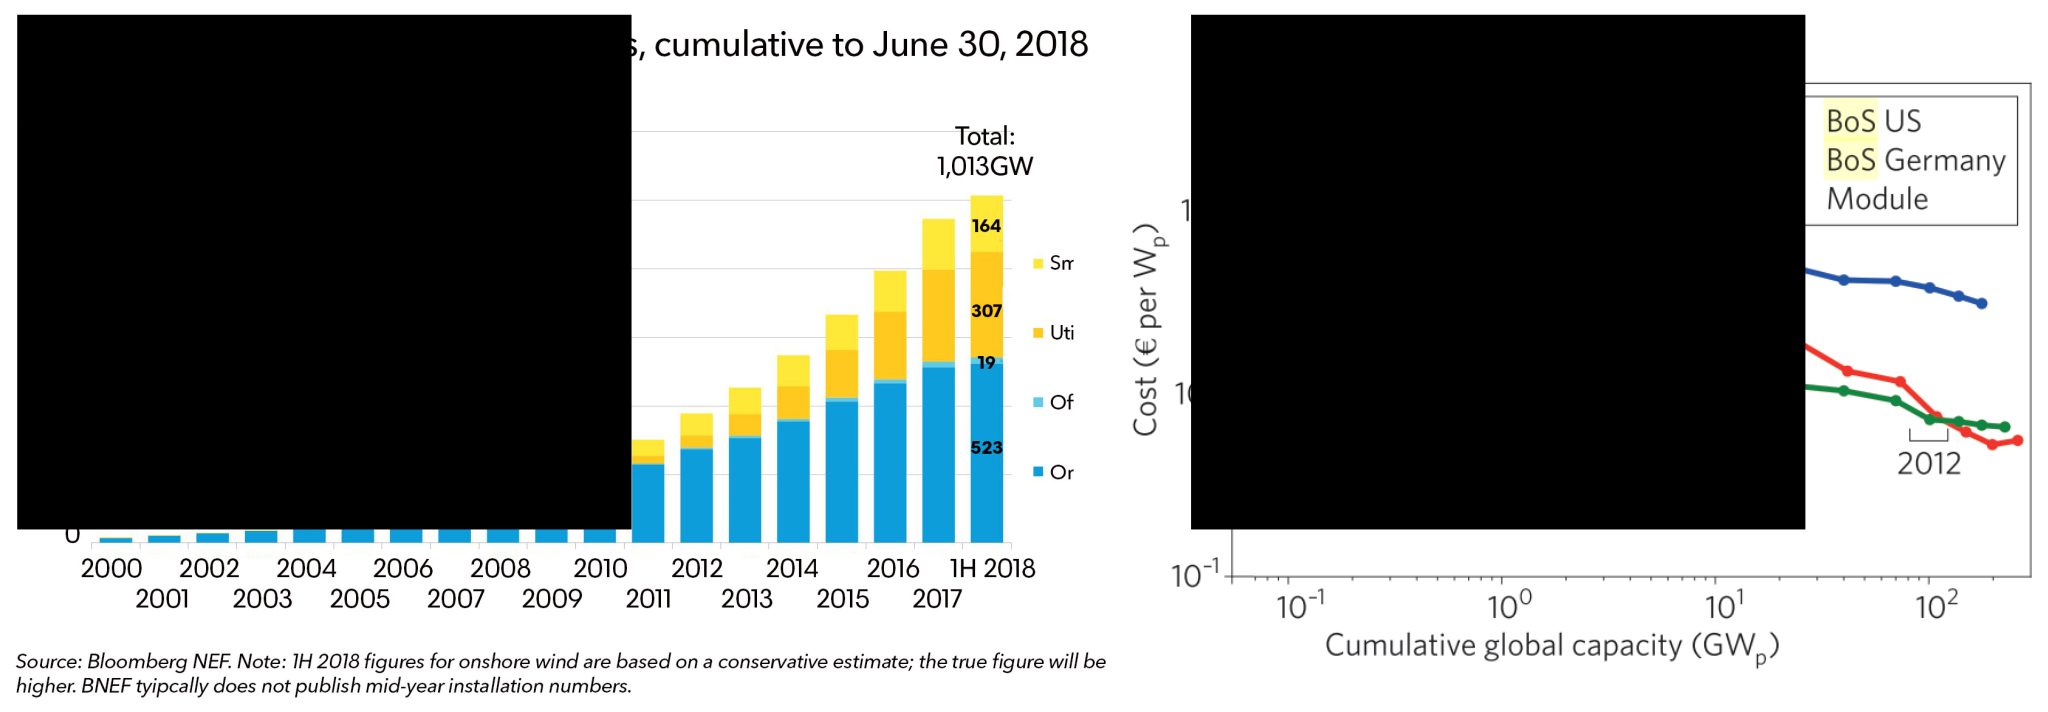
\includegraphics[width=\textwidth]{01_Intro/fig/renewables.png}
	\caption{Rapid progress of renewables. \textbf{(a)}, Growing installed capacity of wind and solar, from Bloomberg New Energy Finance (BNEF), 2019, ref. \citen{BNEF2018}. \textbf{(b)}, Solar learning curve including module and balance of system (BOS) prices, adapted from Creutzig et al, 2017, ref. \citen{Creutzig2017}.}
	\label{fig:renewables}
\end{figure}
Figure \ref{fig:renewables} illustrates the rapid growth in wind and solar energy. The combined installed capacity of wind and solar passed 1 TW\cite{BNEF2018} in 2018, corresponding to approximately one sixth of total electricity generation capacity \cite{IRENA2019}. The actual share of global electricity generated by wind and solar in 2018, though, is only 7.5\% (2000 out of 27000 TWh)\cite{Enerdata2019}, slightly less than half as large a portion as installed capacity. This discrepancy is no quirk in the data - it is a fundamental drawback of wind turbines and solar panels: they only generate electricity when the wind is blowing or the sun is shining, respectively. (More on that in a moment.)

Wind and solar are expected to keep growing as a share of renewable energy generation for some time. The levelized cost per energy is already less than fossil fuels in most places and continues to fall as the total installed capacity increases\cite{Bloomberg2016, Creutzig2017}. Wind and solar electricity generation is an incredible ongoing success story. This is not least because reducing the carbon intensity of electricity works without requiring anything of the consumer, and thus represents a strategy to mitigate the risks of climate change with minimal disruption of society. Indeed, the most promising way to decarbonize many of the other sectors in Figure \ref{fig:sectors} is to \textit{electrify} them. 

Wind and sunlight may come for free, and building wind and solar capacity is now even cheaper than fossil fuel generation, but in the end the changes required by Definition \ref{d:Paris} still don't come for free. And this is because of the \textit{intermittency problem}, namely the fact that the wind and the sun are not kind enough to blow and shine exactly when we might need the electricity. It turns out that there are no cheap solutions to this problem, which will be described in more detail in the next Section. 

One possible rough answer to Question \ref{q:how} is then:

\begin{enumerate}
	\item Install wind and solar as much and as fast as possible to decarbonize electricity production!
	
	\item Electrify everything that can possibly electrified! The main opportunities are in Buildings (6.4\% of direct \ch{CO2} emissions), Transport (14\%), and Industry (21\%). \label{it:electrify}

	\item Solve the problem of intermittancy. \label{it:intermittant}
	
	\item Do less of the things that are hard to electrify, and \textbf{stop doing the greenhouse-gas-emitting things that can't be electrified!} \label{it:sacrifice}
%	\begin{itemize}
%		\item Stop eating meat
%		\item Stop flying
%	\end{itemize}
\end{enumerate}

These four steps can and must be advanced simultaneously.
\footnote{Note that bio-energy is not included in this suggested answer at all. This is in part because bio-energy is out of the scope of this Thesis, but mainly because the climate impact of substituting fossil fuels with biofuels is highly scrutinized. Use of land for bio-energy, especially forest bio-energy may actually \textit{increase} \ch{CO2} concentrations in the atmosphere to 2050 and beyond compared to burning fossil fuels and leaving the biomass to grow.\cite{Searchinger2018, Bentsen2017}. As such, it is a terrible mistake that the EU counts forest biomass as carbon-free renewable energy!}
The challenges are both technological and social. The technological challenges, today, are primarily in Items \ref{it:electrify} and \ref{it:intermittant}. The solutions to the intermittancy problem and for electrifying other sectors are overwhelmingly based on \textit{electrochemistry}, the subject of the next Section and the motivation for this PhD Project.

The societal challenges lie in getting people to accept the costs of implementing these technologies, through taxes and/or increased prices in electricity and other products; and in making lifestyle changes where electricity can't help, or can't help fast enough (Item \ref{it:sacrifice}). Notable carbon-intensive activities that cannot be electrified in the foreseeable future, if at all, include meat consumption (8.5\% of global emissions \cite{Caro2017}) and air travel (2-5\% of global emissions and growing\cite{CarbonBrief_aviation, Larsson2018}, and probably a much larger portion of the emissions for which the reader of this Thesis is responsible). A powerful and indiscriminate way to promote all of the steps above within the framework of a free-market economy and to get individuals to make the necessary sacrifices with minimal intrusion is a universally applied \ch{CO2} tax. This is the favored method by economists\cite{CarbonTax_Economist}, but has to be high enough to influence both corporate and individual behavior.

The need for everyone to accept such sacrifices is where the climate crisis poses a challenge for capitalistic liberal democracies.
\footnote{For a fascinating philosophical discussion of these challenges, Danish readers should read ``Klimakrisens R\o dder'' by Anders Bodin, ref. \cite{Bodin2019}.} 
On the one hand, such societies feature political and economic systems which all too easily fall to the temptation of serving short-term interests. On the other hand, at the core of their values lie the free inquiry of science and the engagement of the public which which have succeeded in driving climate change mitigation to the top of the agenda in Europe. There is no guarantee we will be able to make the necessary changes fast enough to keep climate change from delivering the fatal blow to Fukuyama's dream. But there is reason to be optimistic.


%There is almost certainly no getting around it: For the first three steps to be sufficient, it would require 100\% renewable electricity generation together with more than 60\% overall of all the transport, industry, and buildings direct emissions being eliminated by electrification by 2030. Complete decarbonization of electricity by 2030 is probably possible but expensive: the larger the renewable energy penetration, the more expensive it is to solve the intermittency problem\cite{Budschak2013, Sgobbi2016}. But a 60\% decarbonization of the other sectors, especially industry, seems difficult. 
 







%\section{The carbon cost of this PhD} % moving to last chapter

\section{Electrocatalysis: An important little piece of the solution}\label{sec:our_part}



\begin{itemize}
	\item Transport: more reliance on electric-powered trains, battery vehicles, and hydrogen fuel cell vehicles. Eventually, use electrical energy to make fuels for heavy transport.
	
	\item Buildings: replace fuel heating with electric heat pumps
	
	\item Industry: When possible, replace thermal processes with electrochemical processes. Use electrical heating for others. When possible, replace fossil fuel reactants with electrochemically produced hydrogen.
\end{itemize}

\begin{itemize}
	\item Overcapacity of renewable generation, geographic diversification
	
	\item Flexible grid elements including battery vehicles
	
	\item Hydrogen energy storage
\end{itemize}\clearpage

%

\chapter{The Right Tools to Answer the Right Questions}\label{ch:Tools}

%\section{test}
%\subsection{testest}


As described at the end of the previous Chapter, electrochemistry will play a central role in a steady-state civilization where all of the inputs to our energy infrastructure and chemical industries are renewable or closed-cycle. This will require the development of a wide range of new electrochemical processes and technologies, and the transition will be accelerated by increasing the efficiency and lowering the cost of existing electrochemical technologies, first and foremost water electrolysis. Central to these technologies are the electrode materials, or electrocatalysts, on which the electrochemical half-reactions in Table \ref{tab:EC_overview} take place. Research efforts around the globe have therefore flourished in recent years to develop new electrocatalyst materials and to improve the understanding of existing electrocatalyst materials\cite{Lewis2007, Chu2016, Seh2017}. While (it can not be repeated enough) no realistic pace of progress in these efforts could remove the necessity of high and rising taxes on \ch{CO2} emissions, every bit of progress helps.

It is essential in electrocatalysis development to be sure that the reaction taking place is actually the desired reaction. This sounds obvious, but in electrochemistry it can be tempting to just measure the electrode current (the rate at which \ch{e-} are released or consumed) and not analyze the chemical products. Examples of when the electrode current can be misleading in oxygen evolution catalysis are given in Section \ref{sec:see_the_O2}. The need for product detection is even more important in electrochemical reactions which intrinsically have many possible products, such as the \ch{CO2} reduction reaction\cite{Nitopi2019}. In general, we need product detection to determine the \textit{Faradaic efficiency}, or the portion of the electrons transferred, for a specific reaction or product.

There are a number of product quantification methods including, for example, high pressure liquid chromatography (HPLC), gas chromatography coupled to temperature conductivity detection (GC-TCD) or flame ionization detection (GC-FID), nuclear magnetic resonance (NMR), or colorimetric methods which are all suitable for detecting various products of electrochemical reactions. These all have in common, though, that they typically require an electrochemical reaction to be run for some time to build up a concentration of a product. They are, in other words, ex-situ or batch product detection methods. Detecting electrochemical products after a batch reaction, while useful, is tedious and often leaves out the information of how Faradaic efficiencies can change over time, which can help in understanding stability and electrocatalyst fundamentals. For these reasons, we wish for an \textit{in situ}, i.e. continuous or equivalently ``real-time'', product detection. Mass spectrometry (MS), a readily available technology which is described in the start of Section \ref{sec:ECMS}, is a very useful tool in this regard because of its speed, ability to distinguish between molecules (\textit{chemical resolution}), and sensitivity.

Mass spectrometry, however, has the problem that it requires high vacuum, i.e. pressures less than 10$^{-6}$ mbar, to operate well. This is in stark contrast to electrochemical reactions, which are typically studied in aqueous media at ambient conditions. This leads to the \textit{interface problem}, to which we have developed a new solution which involves interfacing the electrochemical environment and the vacuum chamber housing the mass spectrometer using a specially fabricated silicon microchip. I call it \textit{chip EC-MS}, or (since it is the only electrochemistry - mass spectrometry technique used for this Thesis) simply EC-MS. This technique is the main subject of this Chapter and the subject of Paper \ref{Trimarco2018}.

A pervasive idea in catalysis research is that an improved fundamental understanding of how and why the atoms move around on the surface of catalysts during the electrochemical reaction will enable the \textit{rational design} of more efficient, more stable, and less expensive catalysts\cite{Fundamentals}. Electrocatalysis is no exception\cite{Pfisterer2017, Katsounaros2014a, Wuttig2016, Seh2017}. In this effort, virtually no computational or experimental tool known to materials science has gone unturned in the quest to understand specific electrocatalysts and the fundamentals of electrocatalysis. 

Chip EC-MS has certain advantages, including sub-monolayer sensitivity, fast time response, and the ability to quickly dose reactive gases, that make it ideal for fundamental electrocatalytic studies. (It also happens to have some disadvantages, briefly described in \ref{subsec:disadvantages}.) These advantages make it ideal for \textit{stripping experiments}, which probe the adsorbates on a surface by reactive desorption. This is a powerful type of experiment, in a word because the involvement of surface-adsorbed species is effectively the definition of catalysis. Papers \ref{Trimarco2018}, \ref{Winiwarter2019}, and \ref{Scott_Engstfeld2019} feature stripping experiments, and an example is included in \ref{subsec:examples}.

The extremely high sensitivity of chip EC-MS is based on the fact that every molecule of a gas produced at the electrode being studied (such as \ch{H2} or \ch{O2} produced by water splitting) goes through the chip and to the vacuum chamber. This also makes it a fantastic platform for absolute \textit{quantification} in mass spectrometry, in which a mass spectrometer signal is related not just to the concentration of an analyte, but to an absolute number of molecules of an analyte. This is the subject of Section \ref{sec:quantification}, which includes recommended procedures for using EC-MS as a generalized platform for quantitative mass spectrometry.

The final Section of this Chapter brings us to the juicy heart of this Thesis. 

Atoms are in general too small and too quick (when it's not extremely cold) to see them moving around. And there's the annoying problem that, in general, you can't tell two atoms of the same element apart, so it's impossible to keep track of them! If we wish, experimentally, to understand how atoms move around on an electrocatalytic surface, it is therefore very useful to be able to \textit{label} them. This can be done using \textit{isotopes}, which are versions of an element that have different number of neutrons, and thus different masses. Since chemistry is dominated by protons and electrons (the number of which defines the element), different isotopes of the same element behave (to a reasonable approximation) identically in electrocatalytic reactions. A mass spectrometer, though, can tell the difference! There are a number of exciting things to look at in electrocatalysis with isotope labeling and a sensitive enough setup. Two examples are given in Section \ref{sec:isotopes}, and isotope labeling experiments are the primary focus of the following Chapter.



\section{Electorchemistry - mass spectrometry}\label{sec:ECMS}

Mass spectrometry is one of the most versatile and widely used analysis tools in science\cite{Gross2007, Harris2010}. It also has rich and fascinating history\cite{Griffiths2008}, some notable points in which are summarized in Figure \ref{fig:MS_timeline}. In essence, mass spectrometry is the study and use of methods to separate charged particles in high vacuum by their mass-to-charge (m/z) ratio. The mass-to-charge ratio of  all molecular and atomic ions (at non-relativistic energies) is very close to an integer multiple of one atomic mass unit per fundamental charge, i.e. $q_\text{e}/[1 \text{amu}]$, and so the m/z ratio is usually stated simply as an integer with the implied units of [atomic mass unit per fundamental charge]. Some mass spectrometers have such high resolution that they can separate ions with the same nominal (integer) m/z ratio\cite{Gross2007}, but for the quadrupole mass spectrometers used in this PhD thesis, m/z is in effect an integer.

\begin{figure}[h!]
	\centering
	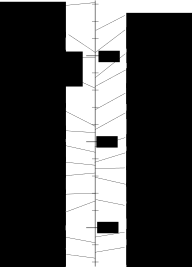
\includegraphics[height=0.8\textheight]{02_Tools/fig/MS_timeline.png}
	\caption{Brief history of mass spectrometry. Most events are described in ref. \citen{Griffiths2008} and at \url{https://en.wikipedia.org/wiki/History_of_mass_spectrometry}. Several later events focus on the coupling of electrochemistry and mass spectrometry: [A], ref. \citen{Hoch1963}; [B], ref. \citen{Bruckenstein1971}; [C], ref. \citen{Wolter1984}; [D], ref. \citen{Wonders2006}; [E], ref. \citen{Henriksen2009}; [F], ref. \citen{Trimarco2015}: [G], Paper \ref{Trimarco2018}.}
	\label{fig:MS_timeline}
\end{figure}

The early development of mass spectrometry was inseparable from the fundamental study of how charged matter behaves under electric and magnetic fields in vacuum, and thus closely tied to many fundamental discoveries in early physics. This includes the discovery of the electron, the discovery of relativistic effects, and the discovery of isotopes. Mass spectrometry has been put to use in an astounding number of applications, including a prominent unsavory one: a modified mass spectrometer was used in one of the purification steps of \ch{^{235}U} for the first atomic bombs (diffusion-based methods and centrifugation have since become much more practical methods of separating isotopes)\cite{Hewlett1962}. Other applications include, for example, trace element analysis (ICP-MS) and protein sequencing (MALDI-TOF).

\begin{figure}[h!]
	
\includegraphics[width=\textwidth]{02_Tools/fig/MS_diagrams.png}
	\caption{Diagram of the components of a quadrupole mass spectrometer (QMS): \textbf{(a)}, electron impact ionization; \textbf{(b)} quadrupole mass separation; and \textbf{(c)},  secondary electron multiplier detection. Adapted from J. Gross, ``Mass Spectrometry'', ref. \citen{Gross2007}. Figure numbers in the image refer to that textbook.}
	\label{fig:MS}
\end{figure}

A mass spectrometer consists of at least three components in a vacuum vacuum chamber\cite{Gross2007}: 

\begin{enumerate}
	\item \textbf{Ion source.} The ion source for the electrochemistry-mass spectrometry (EC-MS) setups described in this Thesis is electron impact ionization (EI, Figure \ref{fig:MS}a). An electron beam is generated by heating up a filament until the high-energy tail of the Fermi distribution of the electrons in the material exceeds the work function of the material. This expels electrons into the vacuum. These electrons are accelerated through a voltage $V$ and pick up an \textit{ionization energy} of $q_\text{e}V$. The ionization energy in this diagram, and throughout this Thesis, is 70 eV. The electrons encounter the molecules to be analyzed (we'll get back to how these molecules got there) in an \textit{ion volume} and impact some of them, imparting a large energy. Many of these impact events result in the expulsion of another electron (or multiple electrons), generating a positively charged ion. Many also result in \textit{fragmentation}, or breaking of the molecules' bonds. It is these \textit{fragments} which are separated and detected by m/z ratio. First they are accelerated from the ion volume to the mass separator.
	
	\item \textbf{Mass separation.} For the EC-MS setups, this is accomplished by a quadrupole (Figure \ref{fig:MS}b). A quadrupole consists of four parallel rods separated by a distance on the order of a centimeter. The rods are connected in two pairs, which are biased by a constant DC bias superimposed on a radio-frequency AC bias. The result is that ions of a specific m/z ratio, which is a function of these two biases, are driven in a stable circular trajectory between the rods and in the plane perpendicular to the rods, whereas ions of other m/z ratios are thrown out by either the AC bias (small ions) or the DC bias (large ions). Ionized fragments enter the four rods with a velocity parallel to the rods, and those with the right m/z ratio fly in neat spirals long enough to make it through. The biases can be changed quickly to scan through a range of m/z ratios (for a \textit{mass spectrum}) or jump between specific m/z ratios of interest to monitor their signals as a function of time (for a \textit{mass-time} measurement). The separation power increases with the length of the quadrupole, and 10 cm is a typical length. 
	
	\item \textbf{Detection.} The ion fragments that make it through the quadrupole hit a detector. In the simplest case, called a \textit{Faraday cup} the detector is just a grounded piece of metal, and the current from the ground, which is equal to the current due to the ions hitting the detector, is measured. However, for higher sensitivity, with a \textit{secondary electron multiplier} (SEM), the ions hit the first of a series of charged plates, starting an electron cascade. The current coming out of the last plate, which is orders of magnitude larger than than the ion current hitting the first plate, is recorded as the \textit{mass spectrometer signal}. For the EC-MS setups in this Thesis, we use a SEM.
\end{enumerate}

Each of the three steps above necessitate high vacuum\cite{Gross2007, PfeifferKnowhow}. 
%(1): The mean free path of electrons should be greater than the distance from the filament to the center of the ion volume, generally a few centimeters,  necessitating a vacuum better than $\sim 10^{-4}$ mbar\cite{Concepts2003}. Furthermore, the lifetime of the filament is decreased significantly at pressures higher than about $\sim 10^{-5}$ mbar. More importantly, the density of ions should be small enough that their mutual repulsion is insignificant compared to the acceleration forces. This begins to be violated when the pressure exceeds $\sim 10^{-6}$ mbar, and the resulting \textit{space-charge effects} cause the signal to no longer respond linearly with the amount of analyte\cite{PfeifferKnowhow, Harris2010}. (2): The mean free path of ions in the vacuum chamber should be significantly greater than the length ($\sim10$ cm) of the quadrupole, necessitating a vacuum better than $\sim 10^{-4}$ mbar\cite{Concepts2003}. (3), The lifetime of the secondary electron multiplier is decreased significantly at pressures higher than about $\sim 10^{-5}$ mbar.
The coupling of mass spectrometry and electrochemistry, motivated at the start of this Chapter, therefore requires an interface allowing electrochemical products from a wet, ambient-pressure environment to enter a vacuum chamber while maintaining a pressure less than $\sim 10^{-6}$ mbar.

Our version of electrochemistry - mass spectrometry involves making the interface between the liquid electrolyte and the vacuum chamber with a specially fabricated silicon microchip called the membrane chip. This strategy gives a number of unique advantages, and also some disadvantages, which make it ideal for fundamental studies but (in its present implementation) less ideal for high-current \textit{in-operando} studies. For the latter type of study, conventional flow-cell differential electrochemistry - mass spectrometry (DEMS)\cite{Baltruschat2004} retains some advantages. Ours should therefore be thought of as a distinct technique, which we refer to as \textit{chip EC-MS} or just \textit{EC-MS}.

\subsection{Chip EC-MS: working principle}\label{subsec:ECMS}

This Subsection will be brief because the motivation, design principles, and original implementation of Chip EC-MS are described extensively in a fantastic PhD Thesis by Daniel Trimarco (ref. \cite{Trimarco2017_PhD}) and in the article which we wrote together, included in this Thesis as Paper \ref{Trimarco2018}. 


\begin{figure}[h!]
	\centering
	\includegraphics[width=\textwidth]{02_Tools/fig/chip_ECMS_diagram.png}
	\caption{\textbf{(a)} Schematic diagrams of chip-based EC-MS and photographs of the membrane chip, adapted from Paper \ref{Trimarco2018} \textbf{(b-c)} Visual microscopy images of the (a) front of the chip showing the membrane, scale bar = 20$\mu$m and (b) back of the chip showing the capillary through the transparent Pyrex, scale bar = 200$\mu$m.}
	\label{fig:chipECMS}
\end{figure}

Figure \ref{fig:chipECMS} includes schematic diagrams of the key components of chip EC-MS. Membrane chips are fabricated at wafer-scale from semiconductor-on-oxide (SOI) wafers with standard clean-room techniques. Photographs of the front and the back of the chip, are shown in the bottom right corner. The photograph of the front of the chip is colorful due to the diffraction of visible light by the chip's membrane. The membrane consists of thousands of holes with a diameter of 2.5 $\mu$m patterned over a circle 7 mm in diameter by UV lithography. Below the membrane is an empty volume, called the \textit{sampling volume} formed by etching of the SOI's oxide layer. The sampling volume is connected to the back of the chip by four holes formed by deep reactive ion etching (DRIE) from the back. A series of gas channels are formed on the back by UV lithography: a wide carrier gas reservoir channel connecting the carrier gas inlet to the carrier gas outlet (indicated in blue in the chip schematic at the top right of Figure \ref{fig:chipECMS}a, three carrier gas delivery channels (intended to achieve symmetric gas flow - indicated by one green channel in the schematic), and a capillary connecting to the mass spectrometer inlet (red in the schematic). These gas channels are sealed by anodic bonding to a Pyrex glass wafer, such that the finished chip is silicon on the top and glass on the bottom. The holes for the carrier gas inlet, carrier gas outlet, and mass spectrometer inlet are formed in the Pyrex with a \ch{CO2} laser prior to bonding. This membrane chip design is protected by a patents\cite{Trimarco_Patent} and commercialized by Spectro Inlets ApS.

\begin{figure}[h!]
	\centering
	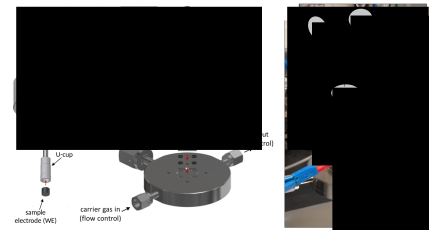
\includegraphics[width=\textwidth]{02_Tools/fig/chipECMS_diagrams_2.png}
	\caption{Diagrams of \textbf{(a)} the cell + working electrode assembly and \textbf{(b)} The cell + chip + interface block assembly. \textbf{(c)} Photo of the setup in use. From Paper \ref{Trimarco2018}}
	\label{fig:chipECMS2}
\end{figure}

The membrane chip is intended as a \textit{window} into what is happening on (or more specifically, what is desorbing from) the surface of an electrochemical sample. This requires the establishment of a three-electrode setup with the working electrode parallel to and close to the membrane. We accomplish this with an \textit{EC-MS cell}, diagrammed on the top-left of Figure \ref{fig:chipECMS}a and in Figure \ref{fig:chipECMS2}a. The cell is most simply described as a piece of polychlorotrifluoroethylene (PCTFE or Kel-F) with holes machined in it. The holes include a cavity through the center for the working electrode assembly. We use the Change-Disk RDE equipment commercially available from Pine Research Instruments for quick and versatile sample exchange. This system uses a PTFE U-cup, which is squeezed slightly between the sample and the cell, to hold the sample in place. The sample can be any 5 mm disk. The distance between the sample and the membrane of the chip, the \textit{working distance}, is defined by a Teflon spacer, and is 100 $\mu$m throughout this Thesis. The volume between the surface of the working electrode and the membrane chip is called the \textit{working volume}. The concentric 7 mm membrane and 5 mm membrane give rise to a 1 mm x 100 $\mu$m \textit{edge volume}. The high aspect ratio of this edge volume ensures that little to no analyte produced at the electrode is lost by lateral diffusion. 

The internal volume of the cell is connected via channels in the EC-MS cell to threaded openings at the top, which are generally fitted with Luer adapters for interfacing with liquid pathway components. In two of these, we place a piece of custom-made glassware with a Luer tip, a ceramic frit to prevent convection, and a large cylindrical volume above. These glassware house the reference and counter electrodes. The other two openings are then used as electrolyte inlet and outlet. To avoid bubbles, the cell must be filled with electrolyte through the inlet before the reference and counter glassware are inserted.

As mentioned at the start of this chapter, chip EC-MS has two great advantages over conventional systems for fundamental studies in electrocatalysis:

\begin{enumerate}
\item Extremely high sensitivity. This is possible because the chip membrane serves as an equilibration step, letting volatile gases evaporate without sucking in solvent. The very low solvent flux means that no differential pumping stage is necessary, unlike DEMS. Furthermore, the low solvent flux is the reason it is possible to run long experiments without flowing electrolyte. Together, this means that \textit{every molecule of volatile product produced on the electrode will make it to the mass spectrometer} 

\item The ability to quickly dose and purge reactant gases. This is possible because the equilibrium of the gas-liquid interface at the chip's membrane works both ways: dissolved gases are released, and the gas fed into the chip saturates the working volume.
\end{enumerate}

Since electrolyte is not flowed during experiments, the cell is a a \textit{stagnant thin-layer} cell. The working volume functions as a perfect diffusion layer, making it relatively easy to model mass-transport in the system. This mass-transport model was first presented in my Master's Thesis\cite{Scott2016_MSc}, and later refined and verified experimentally in Paper \ref{Trimarco2018}. I will not redevelop the model here, but I will use its results from time to time throughout this Thesis.

\subsection{Chip EC-MS: implementation}\label{subsec:setups}

In practice, an external system for vacuum and gas handling is needed to realize the advantages of high sensitivity and quick reactant gas dosing and purging made possible by chip EC-MS. This Subsection describes two such vacuum systems that I worked on during this PhD project. The vast majority of my work was done on the so-called ``Sniffer setup'' at DTU. During my external stay in professor Zhenhai Wen's group at the Chinese Academy of Sciences (CAS) in Fuzhou, I designed a more compact version, which became the EC-MS 200A. A reader who is not interested in these practical details may wish to skip this Subsection. 

In the spirit of making this Thesis useful to my colleagues, Appendix \ref{app:instructions} describes procedures for changing chip and changing carrier gas for each of these setups with reference to the valve diagrams.

\vspace{1cm}
\textbf{\large The Sniffer Setup at DTU:}

\begin{figure}[h!]
	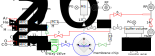
\includegraphics[width=\textwidth]{02_Tools/fig/setup_sniffer.png}
	\caption{Valve diagram of EC-MS setup at DTU. Adapted from Paper \ref{Trimarco2018}. Red: components installed since that publication. Green: The 6-way valve was removed since then as well as the pneumatic valves before the pressure controllers, which were re-purposed. Blue: The interface block, as well as the valve right before it, were replaced to minimize the intervening volume, enabling faster exchange of gases.}
	\label{fig:sniffer}
\end{figure}
Figure \ref{fig:sniffer} shows a valve diagram of the sniffer setup. Most of this setup was built during Daniel Trimarco's PhD project\cite{Trimarco2017_PhD}, and described in Paper \ref{Trimarco2018}. Colors indicate the parts that I have removed (green) or added (red) since its publication.

On the right of the diagram are mass flow controllers (MFC's) which can be used to switch between up to four gases at time (to switch from f.eks. Ar and He requires pumping down behind the MFC through a line not shown). Moving right, we refer to the volume between Valves 7, 8, 9, 10, 11, and 12 and PC 1 as the \textit{gas manifold}. The gas manifold can be evacuated through Valve 7 and filled up from one of the MFC's while regulating the pressure with PC1.

Carrier gas from the gas manifold enters the interface block via Valve 8. The interface block guides it through the carrier gas reservoir channel of the chip, from which it fills the chip's sampling volume and saturates the electrochemical environment. Fast carrier gas exchange thus requires that the volume between valve 8 and the chip, the \textit{carrier gas inlet volume} is as small as possible. This is because the carrier gas inlet volume, unlike the gas manifold, cannot be pumped down, as the resulting vacuum in the sampling volume of the chip would suck in electrolyte. The design of the carrier gas inlet volume can also be optimized with regards to flow patterns to minimize mixing of the old and new carrier gas. 

We refer to the volume between PC1, PC2, and Valves 1, 5, 6, and 7 as the \textit{pumping manifold}. There are actually three possible ways to pump on the pumping manifold: (1) Directly to the \textit{roughing pump} (RP) through Valve 6, (2-3) or through a buffer volume and then a \textit{turbo molecular pump} (TMP or just turbo pump) via either a (2) valve 2 and a needle valve or (3) a gate valve. Of these options, the direct roughing pump connection is the only one that can quickly remove a large amount of gas, as this would damage the turbo pump. Valve 14 should be closed while gas is fed directly to the roughing pump, as the pressure behind the turbo pump must also be kept low during operation. On the other hand, the turbo pump is required to reach high vacuum, which it can do slowly for a moderate amount of gas through the needle valve or quickly for a small amount of gas through the gate valve.

During operation, carrier gas is flowing from the gas manifold to the pumping manifold through the chip, and its pressure is regulated by PC2, which is set to 1 bar for all of the experiments in this Thesis. Excess carrier gas flows through PC2 to the pumping manifold where it is ultimately removed through the roughing pump, typically via the buffer volume and needle valve, so that valve 14 can remain open.

When a new chip is installed, the \textit{post-capillary volume} bound by the chip, Valve 13, and Valve 5 is vented to atmospheric pressure. The post-capillary volume must then be pumped down to high vacuum again through valve 5 and the pumping manifold before valve 13 can be opened, connecting the experiment to the mass spectrometer. The mass spectrometer is always held at high vacuum by its own designated turbo and roughing pumps.

The procedures for chip pump-down and carrier gas exchange are described in Appendix \ref{app:sniffer}

\vspace{1cm}
\textbf{\large The ECMS-200A in Fuzhou:}

\begin{figure}[h!]
	\centering
	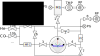
\includegraphics[width=0.75\textwidth]{02_Tools/fig/setup_Fuzhou.png}
	\caption{Valve diagram of EC-MS setup at Fuzhou. In reality, at the time of writing this thesis, the pressure controller is actually a modified pressure regulator, which works but is not as stable.}
	\label{fig:Fuzhou}
\end{figure}

The sniffer setup described above can be considered a ``delux setup'' with an excess of components to maximize functionality. The group in Fuzhou asked me to design a ``budget setup'' which captured the central advantages of chip EC-MS with as few components as possible. They then built my design, shown in Figure \ref{fig:Fuzhou} with the outside help from a Chinese mass spectrometer company, Quantang Instruments. Much to my frustruation, Quantang built a box around the valve system, making it quite tedious to make changes to the system, and put their logo and the name ECMS200A on the box.

All of the concepts are the same as for the sniffer setup, but the operation is different. The procedures for chip pump-down and carrier gas exchange are described in Appendix \ref{app:Fuzhou}. The cost of having one less Turbo pump is the need to wait for long pumping periods and to turn off the filament of the mass spectrometer when changing chips. The carrier gas exchange procedure is actually slightly simpler than that of the sniffer setup and saves three MFC's and a PC. The only disadvantage is that, with only one MFC, it is not easy to prepare a controlled gas mixture (a functionality I have rarely used on the sniffer setup).

\vspace{1cm}
\textbf{\large Spectro Inlets:}

\begin{figure}[h!]
	\centering
	\includegraphics[width=0.75\textwidth]{02_Tools/fig/spectro.png}
	\caption{Photos of the setup at Spectro Inlets ApS. From their website: \url{https://spectroinlets.com/}}
	\label{fig:spectro}
\end{figure}
Finally, I should mention that there is now a commercially available setup which combines the best of both worlds: The great functionality of the Sniffer setup and the simplicity and compactness of the ECMS200A. This is made possible in part due to some custom vacuum components. The setup, sold by Spectro Inlets ApS, is shown in the photographs in Figure \ref{fig:spectro}. I have been involved in conversations aiding the development of this setup, as a kind of test user, but can't go to detail here on its design. The Spectro Inlets setup also comes with a software automating the chip pump-down and carrier gas exchange procedures. The procedures described in Appendix \ref{app:instructions} for the other two setups are thus simplified to pressing a button.


\subsection{Example experiments: RHE potential measurement and CO stripping}\label{subsec:examples}
Here I show two examples of common electrochemistry experiments as seen through the window of chip EC-MS. These two experiments also demonstrate the utility of the gas-exchange functionality, and happen to be quite interesting when instead done in isotope-labeled electrolyte. Isotope-labeled versions of these two experiments are shown later in this Chapter, in Subsections \ref{subsec:isotope_RHE} and \ref{subsec:isotope_CO2}.

The first experiment is a measurement of the reference electrode potential on the reversible hydrogen electrode (RHE) scale. The reversible hydrogen electrode potential is defined as the potential at which the hydrogen evolution and hydrogen oxidation reactions (HER and HOR, respectively) are at equilibrium in electrolyte saturated by 1 bar hydrogen:
\begin{equation}
\ch{2 (H+ + e- ) <-> H2} \label{rxn:HER2}
\end{equation}
This situation can be easily created in a chip EC-MS setup using hydrogen as the carrier gas and a platinum electrode as the sample, since platinum is an excellent catalyst for the HER/HOR\cite{Nørskov2005a, Kemppainen2015, Tymoczko2016}. 

\begin{figure}[h!]
	\centering
	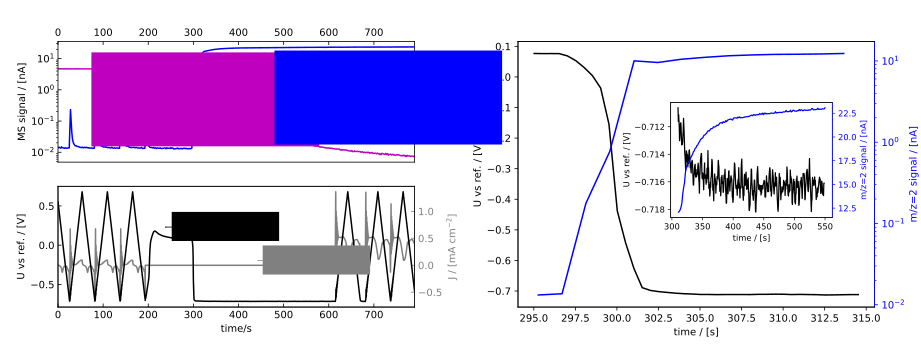
\includegraphics[width=\textwidth]{02_Tools/fig/RHE_calibration.png}
	\caption{RHE calibration experiment using a polycrystalline platinum electrode in 0.1 M \ch{HClO4}. \textbf{(a)} EC-MS plot with mass spectrometer signals in the top panel and the concurrent electrochemical data in the lower panel. \textbf{(b)} A zoom-in on the time at which the carrier gas is switched from helium to hydrogen while the electrode is at OCP, showing the electrode potential (black, left y-axis) co-plotted with the m/z=2 signal (blue, right y-axis)}.
	\label{fig:RHE_cal}
\end{figure}

The experiment is shown in  in Figure \ref{fig:RHE_cal}a as an \textit{EC-MS plot}, in which the electrochemical potential (left y-axis) and current (right y-axis) are plotted against time in the bottom panel and the concurrent mass spectrometry data is shown in the top panel on the same time axis. (Customized EC-MS plots, including all of the ones presented in this Thesis, can be produced in one line of code with the highly versatile \texttt{plot\_experiment} function of the \ch{EC\_MS} python package, described in Appendix \ref{app:EC_MS}.)

Starting from the left: the platinum electrode is cycled between -0.7 and +0.7 V vs the reference electrode (Hg/\ch{HgSO4}) in helium-saturated electrolyte. Three full cycles are shown. Hydrogen is produced near the cathodic potential limit, giving rise to an increase in the mass spectrometer signal at m/z=2. The electrode is set to open-circuit potential (i.e., the current is set to zero) at the cathodic potential limit of the fourth cycle. This results in less \ch{H2} than the first cycles, since in the first cycles HER continues at the start of the anodic scan. The open-circuit potential then drifts in the anodic direction until just before the onset of \ch{$*$ OH} adsorption, which would draw current. At 300 s, \ch{H2} is flowed through the chip, replacing \ch{He} in the carrier gas reservoir channel. The \ch{H2} very quickly enters the sampling volume of the chip, giving rise to a m/z=2 signal in the mass spectrometer. Simultaneously, the \ch{H2} saturates the electrolyte in the working volume. The first \ch{H2} molecules to encounter the electrode are immediately oxidized to \ch{H2O} because there is a substantial overpotential to drive the HOR (Reaction \ref{rxn:HER2} in the leftwards direction). However, since the electrode is at OCP, there is nowhere for the resulting electrons to go, and so they change the charge density of the electrochemical double layer, which functions as a capacitor\cite{Chan2015a}. This causes the potential to drop very quickly. The electrode soon reaches a potential at which Reaction \ref{rxn:HER2} is in equilibrium. This equilibrium potential depends on the partial pressure of \ch{H2}, and so the potential continues to change slowly as \ch{H2} fully replaces \ch{He}. 

The example in Figure \ref{fig:RHE_cal} is unfortunately not the most elegant gas exchange, as indicated by the inflection points in the MS signals as \ch{H2} replaces \ch{He} in Figure \ref{fig:RHE_cal}a. (This results from an overpressure in the gas manifold before opening Valve 8 in Figure \ref{fig:sniffer}, which causes turbulence and gas mixing in the carrier gas inlet volume.) Figure \ref{fig:RHE_cal}b shows the simultaneous change in the \ch{H2} signal and electrode potential during the gas switch. The electrode potential becomes stable to within a few millivolts just 10 seconds after the switch, but the last $\approx$ 2 mV to the RHE potential of -0.717 V vs the reference electrode take about 100 s (inset). This is, nonetheless, a much faster RHE measurement than can be accomplished when a macroscopic amount of electrolyte, for example in an H cell, needs to be fully purged with hydrogen. Such RHE measurements are used routinely to calibrate the reference electrode potential on the RHE scale in a new electrolyte.

\begin{figure}[h!]
	\centering
	\includegraphics[width=\textwidth]{02_Tools/fig/Trimarco2018_fig03.png}
	\caption{Experiments showing HER, OER, CO oxidation, and CO stripping on Pt in 1.0 M \ch{HClO4}.  \textbf{(a)} and \textbf{(c)} show EC-MS plots and \textbf{(b)} and \textbf{(d)} each show two parts of the respective data set co-plotted against potential. \ch{He}, \ch{CO}, \ch{H2}, \ch{O2}, and \ch{CO2} fluxes were obtained by calibrating the m/z=4, 28, 2, 32, and 44 signals, respectively, according to the procedures described in Section \ref{sec:quantification}. For a detailed discussion, see Paper \ref{Trimarco2018}.}
	\label{fig:fig3}
\end{figure}

Figure \ref{fig:fig3}, from Paper \ref{Trimarco2018}, demonstrates platinum electrochemistry involving carbon monoxide (CO). Here, the potential has been calibrated to the RHE scale as described above, and the mass spectrometer signals have been calibrated as described in Section \ref{sec:quantification}. Figure \ref{fig:fig3}a shows a long electrochemistry program including constant-potential steps and cyclic voltammatry, and a switch from He to CO in the middle. It is described in detail in the paper. Two cycles from this program (one in He and one in CO) are selected and plotted vs potential in Figure \ref{fig:fig3}b, as is popular among users of DEMS and OLEMS.

Figure \ref{fig:fig3}c and d show a CO stripping experiment, a common method of characterizing noble metal surfaces in electrocatalysis\cite{Mayrhofer2005, Koper2009, Ganassin2017, Jensen2017_PhD}. It consists of two steps: adsorption of CO, and oxidation of adsorbed CO, given in Reactions \ref{rxn:COads} and \ref{rxn:COstrip}, respectively:
\begin{align}
\ch{CO + $*$ &-> $*$ CO}\label{rxn:COads}\\
\ch{$*$ CO + H2O &-> $*$ + CO2 + 2 (H+ + e- )}\label{rxn:COstrip}
\end{align}
To study the oxidation of surface-adsorbed *CO in isolation, the *CO dosed in the first step has to be purged from the electrolyte before the second step.

In Figure \ref{fig:fig3}c, after an initial cyclic voltammagram, a short pulse of CO is dosed using the 6-way valve in Figure \ref{fig:sniffer} and adsorbs on the surface, as indicated by the CO displacement current at $\approx$190 s. After the CO dose, the first cycle shows no \ch{H2} signal or hydrogen adsorption current (Figure \ref{fig:fig3}d), indicating the surface is fully poisoned by adsorbed CO. The anodic scan shows a CO stripping current starting at $\approx$0.7 V vs RHE. The final cycle is identical to the cycle before the \ch{CO} dose. We like to brag that this is the fastest complete CO stripping experiment ever reported in the literature.

This experiment also demonstrates the sensitivity of the system: the integrated \ch{CO2} signal corresponds to approximately 0.75 ML, i.e. 3 CO molecules adsorbed for every 4 Pt surface atoms; and the integrated \ch{H2} signal at 410 s corresponds to approximately 0.05 ML.

\subsection{Disadvantages}\label{subsec:disadvantages}

The attentive reader might be wondering why the shapes of the \ch{CO2} and \ch{H2} signals in Figure \ref{fig:fig3}c are so different. Whereas the \ch{H2} signal peaks at 10 pmol/s within a second or two of the cathodic potential limit and has completely passed a few seconds after that, the \ch{CO2} signal, which corresponds to $\approx$ 15 times as many molecules, also peaks at $\approx$ 10 pmol/s but then falls very slowly. This is especially annoying when data are plotted against potential (Figure \ref{fig:fig3}d), because the tail of the \ch{CO2} signal lasts well into the cathodic scan, even though all of the \ch{CO2} is produced by the electrode surface during the anodic scan. Since the ability to detect a signal is described by its height as well as its area, chip EC-MS is in effect less sensitive to \ch{CO2} than \ch{H2}.

It turns out that this is an inevitable part of chip EC-MS, inseparable from its major advantage of low solvent evaporation\cite{Scott2016_MSc}. Both are cases of a general fact: the characteristic time for an analyte to leave the working volume and enter the mass spectrometer is strongly dependent on its Henry's-Law constant of volatility. This is defined as the equilibrium ratio of its partial pressure in the gas phase to its concentration in the aqueous phase:
\begin{equation}
K_H^i = \frac{p^i}{c^i}
\end{equation}
Because there is equilibrium across the chip membrane, the partial pressure of a uniformly dissolved analyte in the chip's sampling volume, and thus the rate at which it is removed through the chip capillary, is proportional to its Henry's-Law constant. The characteristic time, taking both diffusion through the working volume and evaporation across the chip's membrane, for removal of analyte $i$ from the working volume is\cite{Scott2016_MSc}:
\begin{equation}
\tau^i = \frac{L^2}{2D^i} + \frac{L p^0_\text{chip}A_\text{el}}{\dot{n}^0_\text{cap} K^i_H}
\end{equation}
where $L$ is the working distance, $D^i$ is $i$'s diffusion constant in water, $p^0_\text{chip}=1$ bar is the total pressure in the chip, and $\dot{n}^0_\text{cap}$ is the combined flux through the capillary. For all but the least soluble gases (including \ch{H2} and \ch{O2}), this is dominated by the second term, which can vary many orders of magnitude. Thus, while any analyte with any vapor pressure will in principle reach the mass spectrometer eventually, detection of liquid products is highly unpractical. The characteristic time is (ref. \cite{Scott2016_MSc} and Paper \ref{Trimarco2018}) 2 s for \ch{H2}, 3 s for \ch{O2}, 27 s for \ch{CO2}, and $2.5\cdot10^{5}$ s for ethanol.

\begin{figure}[h!]
	\includegraphics[width=\textwidth]{02_Tools/fig/fig07_old.png}
	\caption{Model comparing the sensitivity of chip EC-MS to conventional DEMS via the collection efficiency in a hypothetical flow setup. Adapted from Paper \ref{Trimarco2018}.}
	\label{fig:sensitivity}
\end{figure}

Figure \ref{fig:sensitivity} seeks to answer the question of when it is advantageous to use chip EC-MS and when it is advantageous to use conventional DEMS. The question is rephrased in terms of \textit{collection efficiency} in a hypothetical flow setup: if an analyte dissolved in an electrolyte is flowing past the vacuum inlet (essentially the collection chamber in a dual thin-layer flow cell\cite{Jusys1999, Clark2015}), will more molecules of the analyte reach the mass spectrometer if the inlet is chip EC-MS or DEMS? To answer this question, I modified the stagnant thin-layer mass transport model to give the concentration profile in such a flowing collection volume\cite{Scott2016_MSc}. The model is diagramed in Figure \ref{fig:sensitivity}a and three cases are shown in Figure \ref{fig:sensitivity}c-d. The resulting collection efficiencies are plotted as a function of Henry's-law constant in Figure \ref{fig:sensitivity}b. For light gases, chip EC-MS wins due to the lack of a differential pumping stage. For volatile liquids, DEMS wins because the much faster non-equilibrium mass transport of products into the first stage of the vacuum chamber outweighs the loss due to differential pumping. 

Thus, chip EC-MS is not ideal for, e.g., \textit{in-operando} studies of \ch{CO2} reduction, in which production rates can be high but the interesting products are liquid at room temperature.

Furthermore, while the sensitivity and ability to quickly dose reactant gases are major advantages for chip EC-MS in fundamental studies, it should not be considered a full substitute for a rotating disk electrode (RDE) setup or other setup optimized for cyclic voltammatry. It can sometimes be challenging to get good cyclic voltammagrams in the setup. Figure \ref{fig:current_distribution}a shows electrochemistry data from Figure \ref{fig:RHE_cal}a plotted against potential. The magenta cycle is with He as the carrier gas, and the blue cycle is with \ch{H2} as the carrier gas. The \ch{H2} CV is shifted up with respect to the \ch{He} CV due to a mass-transport-limited hydrogen oxidation current until the platinum surface starts to oxidize at 0.9 V vs RHE and becomes less active for hydrogen oxidation. This all makes sense, but the CV's are dominated by an artifact in the start of the anodic scan: rapid oscilations of current and potential. 

\begin{figure}[h!]
	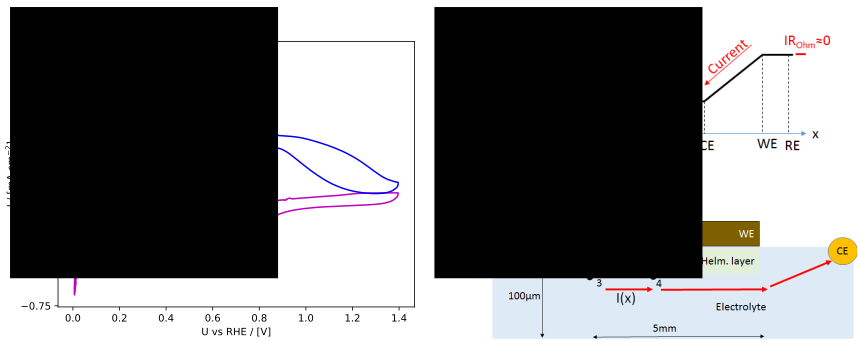
\includegraphics[width=\textwidth]{02_Tools/fig/nonideal_current_distribution.png}
	\caption{\textbf{(a)} CV's in He (magenta) and \ch{H2} from Figure \ref{fig:RHE_cal}. The squiggles are the result of oscillations caused, in part, by electrolytic resistance accross the surface of the sample. \textbf{(b)} Schematic diagrams of electrode connections to the working volume, indicating that while the conventional ohmic resistance is zero, the resistance within the working volume means that the electrochemical potential is not uniform; adapted from my Master's Thesis\cite{Scott2016_MSc}}.
	\label{fig:current_distribution}
\end{figure}

These oscillations are worse the less conductive the electrolyte is, and occur most often when there is a sudden change in absolute current density, such as (in this case) right at the scan polarity change in the hydrogen region. They are attributed to the challenge of controlling the potential when there is a large resistance through the electrolyte from one end of the electrode to the other, first described in my Master's Thesis\cite{Scott2016_MSc}. 

Briefly, the conventional ohmic drop in the EC-MS cell is zero, since the current through the electrolyte is conducted between the working electrode (WE) and the counter electrode (CE), but potential is measured to the reference electrode (RE) on the opposite side of the working electrode (top half of Figure \ref{fig:current_distribution}b. Indeed, PEIS measurements in the sniffer setup show a vertical line through zero resistance on the real axis. This is despite the fact that there are large resistances in the cell, most notably in the working volume itself. This resistance can lead to the potential drop across the Helmholtz layer on two parts of the working electrode not being identical, as indicated in the bottom of Figure \ref{fig:current_distribution}. How exactly this leads to oscillations, I do not fully understand.

I realized remarkably late in my PhD project that setting the bandwidth on the Biologic SP-150 Potentiostat to 3, with everything else set up perfectly, could usually remove this artifact. Before that, I had realized that putting a 100 Ohm resistor behind the working electrode helps. This effectively introduces a conventional ohmic resistance, which seems to help the potentiostat avoid such oscillations, and is easy to correct for afterwards when plotting CV's.

The maximum size of the difference in electrochemical potential across the working electrode is important to know, as it is a possible source of error in activity measurements, such as those that will be presented in Section \ref{sec:low_O2}. For 0.1 M \ch{HClO4} (the electrolyte used in that Section), the resistance from one end of the working volume to the other is on the order of
\begin{equation}
R = \frac{1}{\kappa}\frac{d}{L\frac{d}{2}} = \frac{2}{\kappa L} = \frac{2}{4.2 \left[\frac{\text{S}}{\text{m}}\right]\cdot 100[\mu\text{m}]} = 4.8 [\text{k}\Omega]
\end{equation}
Where $\kappa$ is the conductivity of the electrolyte, $L$ is the working distance, $d$ is the diameter of the disk, and to make sure the resistance is overestimated I've approximated the geometry as a resistor with a cross section of $L\cdot\, d/2$ but a length of $d$. 

This is a huge resistance! The maximum current densities used in this thesis are approximately 100 $\mu$A (0.5 mA/cm$^2$ geometric current density). At this current density, if we assume the worst case, that all of the current comes from the end of the working electrode closest to the reference electrode, then the potential at the end of the working electrode closest to the counter electrode could be off by as much as $100[\mu\text{A}]\cdot4.8 [\text{k}\Omega] = 0.48[\text{V}]$. The error is in the direction to \textit{increase the overpotential} of the current-drawing reaction on the part of the electrode close to the CE compared to what it should be according to the potential difference between WE and RE. This is a huge potential error! 

We are partially saved by two facts:
\begin{itemize}
	\item The worst case scenario is very very far from the truth. In reality, there will be more current from the side of the working electrode closest to the counter electrode. In other words, an uneven current distribution will seek to alleviate an uneven potential distribution, not exacerbate it.
	
	\item The error is reduced at small current densities, which are the interesting ones for chip EC-MS anyway. In the same electrolyte at 1 $\mu$A (corresponding to 10 pmol/s of electrons), the error is less than a worst-case scenario of 4.8 mV difference, still not great but more acceptable.
\end{itemize}

Nonetheless, solving this should be a high priority for continued development of chip EC-MS. A promising solution is to fabricate chips with liquid through-holes, so that a counter electrode can be placed behind the chip and parallel to the working electrode. A first attempt at this is described in the Master's Thesis of Jesper Pan\cite{Pan2018_MSc}, and a second attempt is being led by Thomas Pedersen of DanChip.

To improve the mood after this discussion of problems with chip EC-MS, the next Section will focus on a positive aspect: the fact that 100\% of gaseous electrochemical products make it to the mass spectrometer makes chip EC-MS an excellent platform for \textit{absolute quantification} in mass spectrometry.



\section{Quantitative mass spectrometry: counting molecules}\label{sec:quantification}

This Section lays out procedures for using electrochemistry as a platform for quantification in mass spectrometry. It is a bit of a side story from the main narrative to this Thesis, as well as quite technical. A reader unlikely to use the methods presented here may wish to skip to Section \ref{sec:isotopes}.

Quantification means relating the signal at a mass-to-charge ratio (m/z) or set of m/z's to the amount of the molecule being quantified, the \textit{analyte}. However, \textit{amount} here can have at least two different meanings.

Mass spectrometry is routinely used to analyze the concentration of analytes in a gas or other matrix\cite{Harris2010, Gross2007}. When the desired value is a concentration in a gas, calibrating the mass spectrometer is trivial. One need only flow a standard gas or series of standard gases with a known concentrations of the analyte past the inlet and measure the signal at a m/z value unique to the analyte. The standard gases should otherwise as much as possible resemble the gas which will be tested. In general, the signal will scale linearly with the concentration, giving a sensitivity factor. Such a sensitivity factor has the dimensions of signal per concentration.

In the context of chip EC-MS and certain other applications such as catalyst testing in microreactors, we mean something different. We use the following definition of quantification:

\begin{definition}
	Quantification: Determining, from mass spectrometer signals, the rate (in molecules per second) at which an analyte is entering the vacuum chamber. \label{d:quantification}
\end{definition} 

Equivalently, quantification means being able to determine the number of molecules that entered the vacuum chamber in a given time from the integrated mass spectrometer signal. In chip EC-MS as well as microreactor experiments, this is useful because all of the products of a catalytic reaction can be assumed to enter the vacuum chamber, and we typically wish to determine the number of catalytic turn-overs from the integrated signal or, at steady state, the turn-over rate from the signal. 

The sensitivity factor we are looking for has the dimensions of integrated signal per molecule. If signal is measured in Amperes and molecules are counted in mol, then the sensitivity factor has units C/mol. Mathematically, the sensitivity factor for analyte $i$ at a mass-to-charge ratio (m/z=) $M$ where there are no interferences, is defined as $F^i_M$ such that:
\begin{align}
S_M &= F_M^i \dot{n}^i_{\text{vac}}\,\hspace{1cm}\text{or, by extension,} \label{eq:S}\\
\int_{t_1}^{t_2} S_M \mathrm{d}t &= F_M^i \Delta n_{\text{vac}} \label{eq:int_S}
\end{align}
where $S_M$ is the signal at m/z=$M$, $\dot{n}^i_\text{vac}$ is the molar flux of analyte $i$ into the vacuum chamber, and $\Delta n_\text{vac}^i$ is the amount of analyte $i$ to enter the vacuum chamber between times $t_1$ and $t_2$.

This type of sensitivity factor is more difficult to determine than the signal-to-concentration sensitivity factor because, given a gas with a known analyte concentration, its determination also requires knowledge of the permeability of the vacuum inlet. Estimating the capillary flux is precisely how quantification was originally accomplished for the microreactors \cite{Henriksen2009} and the electrochemical microreactor which was the predecessor to the EC-MS membrane chip\cite{Trimarco2015}. 

Electrochemistry gives a powerful platform for accurate quantification, because there are analytes for which the electrode current can directly tell us $\dot{n}$. The next Subsection will describe electrochemical calibration, and the following Subsections will describe how electrochemical calibrations can be used to validate calibrations based on capillary flux and together extended to allow quantification, as understood in Definition \ref{d:quantification}, of any analyte.

\subsection{Internal calibration by electrochemistry}\label{subsec:internal}

Electrochemical calibration of mass spectrometer signals is based on establishing a steady and known value for $\dot{n}^i$ in Equation \ref{eq:S} based on Faraday's law of electrolysis:
\begin{equation}
\dot{n}^i_\text{el} = \frac{I}{z\mathcal{F}}\,,\label{eq:Far}
\end{equation}
where $I$ is the current, $z$ is the stoichiometric coefficient of electrons (positive for oxidation and negative for reduction) in the electrochemical half-reaction of which $i$ is a product, and $\mathcal{F}=96487$ C/mol is Faraday's constant.

Equation \ref{eq:Far} implicitly assumes that \textit{all} of the current $I$ goes to formation of the product $i$, i.e. it assumes 100\% \textit{Faradaic efficiency}. Its use is thus limited to reactions that can be run at 100\% Faradaic efficiency. In practice, this is a severe limitation on the analytes that can be calibrated directly by electrochemistry. Three of the analytes that can be calibrated directly are \ch{O2}, \ch{H2}, and \ch{CO2}, which can be produced at $\approx$100\% Faradaic efficiency by OER, HER, and CO oxidation, respectively:
\begin{align}
\ch{2 H2O &-> O2 + 4 (H+ + e- )} &&\text{OER}\label{rxn:OER2}\\
\ch{2 (H+ + e- ) &-> H2} &&\text{HER}\label{rxn:HER2p2}\\
\ch{CO + H2O &-> CO2 + 2 (H+ + e- )} &&\label{rxn:COox2}\text{CO oxidation}
\end{align}
\begin{figure}[h!]
	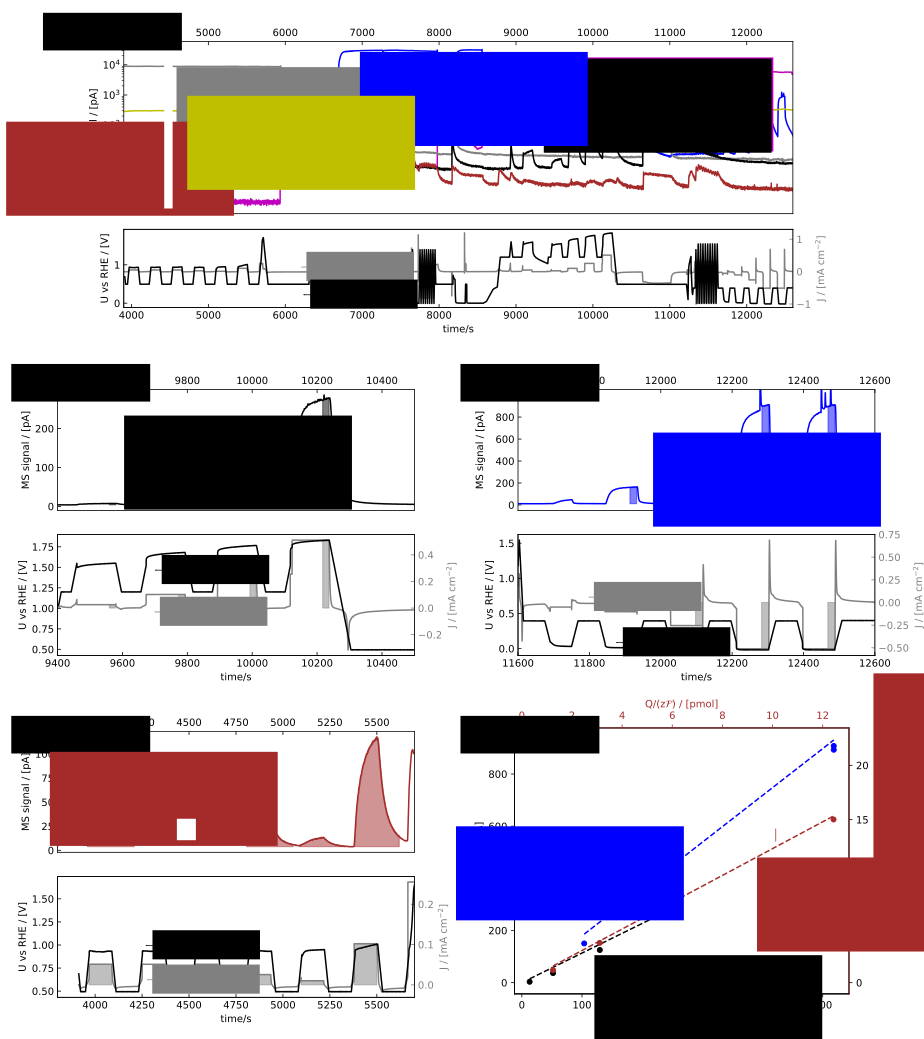
\includegraphics[width=1\textwidth]{02_Tools/fig/internal_calibrations.png}
	\caption{Calibration experiments for \ch{O2} by OER, \ch{H2} by HER, and \ch{CO2} by CO oxidation using a platinum electrode in 1.0 M \ch{HClO4}. \textbf{(a)} The entire experimental dataset. Zoom-ins are shown for the three calibrations: \textbf{(b)}, OER; \textbf{(c)}, HER; and \textbf{(d)} CO oxidation. \textbf{(e)}, The resulting calibration curves are plotted for \ch{H2} and \ch{O2} as near-steady-state signal vs production rate (bottom and left axes), and for \ch{CO2} as integrated signal vs amount produced (top and right axes). The proportionality between the two x-axes and the two y-axes are identical such that the slopes, which are the respective sensitivity factors, are directly comparable.
	}
	\label{fig:internals}
\end{figure}
\clearpage % Otherwise this Figure pushes all the other figures to the end of the Chapter
Figure \ref{fig:internals} shows calibrations for \ch{O2}, \ch{H2}, and \ch{CO2} by these reactions. These calibration data are not as flawless as those in the SI to Paper \ref{Trimarco2018}. They were chosen for this Thesis because, together with the data in Figure \ref{fig:internals_2} below, which were taken on the same day, they include the largest number of directly comparable calibrations. I collected the data in Figures \ref{fig:internals} and \ref{fig:internals_2} together with Anna Winiwarter to obtain a full set of sensitivity factors to calibrate the results of propene stripping experiments that build on the results in Paper \ref{Winiwarter2019}.

The full dataset is shown in Figure \ref{fig:internals}a. From the left: the dataset starts with the electrode in \ch{CO}-saturated electrolyte. The electrode is subject to several periods of 2 minutes of constant-current CO oxidation, inter-spaced by scans to a \textit{resting potential} of 0.5 V vs RHE to separate the peaks. There is a small gap in the MS data around 4500s due to a computer glitch. After the \ch{CO2} calibration, the carrier gas is changed from \ch{CO} to He, and then to \ch{H2} to measure the signal due to \ch{H2} carrier gas flux through the capillary (which will be discussed in Subsection \ref{subsec:capillary}) and to calibrate the reference electrode. (We actually realize after the anodic scan at $\approx$ 7700 s that we had forgotten to strip off the adsorbed \ch{CO} from before, which would have poisoned the electrode for HER/HOR, and so we repeated the RHE calibration.) Then the carrier gas was changed back to \ch{He} for \ch{O2} calibration by OER. Again, we used 2-minute constant current steps inter-spaced by time at a resting potential to get separated peaks in the m/z=32 signal. Then we switched the carrier gas briefly to \ch{O2} to measure the signal due to \ch{O2} carrier gas flux through the capillary, and switched back to \ch{He}. Finally, after cycling the potential to clean off any contaminants that may have adsorbed or deposited on the electrode, we calibrated \ch{H2} by HER, again with constant-current measurements inter-spaced by a resting potential.

There are two ways of extracting a sensitivity factor from calibration data made with constant-current calibration steps inter-spaced by resting periods: differential and integral. For a differential calibration, we chose a time interval over which to make the assumption of steady-state, i.e. 
\begin{equation}
\dot{n}^i_\text{vac} = \dot{n}^i_\text{el}\,,\label{eq:SS}
\end{equation}
and the sensitivity factor $F_M^i$ is, according to Equation \ref{eq:S}, simply the ratio of the signal $S_M$ to the production rate $n^i_\text{el}$, where the latter is calculated by Equation \ref{eq:Far}. For an integral approach, we do not make the assumption of steady state, but instead use the fact that, over time, every gas molecule formed at the electrode will make it to the vacuum chamber:
\begin{equation}
\int \dot{n}^i_\text{vac}\mathrm{d}t = \int \dot{n}^i_\text{el}\mathrm{d}t\,,\label{eq:int}\,
\end{equation}
and then determine $F_M^i$ by Equation \ref{eq:int_S}.

The differential approach is usually good enough for \ch{O2} (Figure \ref{fig:internals}b) and \ch{H2} (Figure \ref{fig:internals}c), which have fast mass transport (Paper \ref{Trimarco2018}) and can reach steady state within a minute. In this particular dataset, the mass transport is rather slow, perhaps due to poor alignment of the electrode, and the respective signals appear to be close to but not quite at steady state. It turns out that it's good enough (using the integral approach results in the same sensitivity factor within 2\%). The highlighted areas of Figure \ref{fig:internals}b and c show the time interval over which the signal was averaged.

For \ch{CO2} (Figure \ref{fig:internals}d), which has much slower mass transport due to its higher solubility in the electrolyte [Paper \ref{Trimarco2018}], we have to use the integral approach. Here, the highlighted areas show the time intervals for which $\dot{n}^{\ch{CO2}}_\text{el}$ (bottom panel) and $S_\text{M44}$ (top panel) were taken. The two calibration points affected by the gap in the MS data were excluded.

The resulting calibration curves are plotted in Figure \ref{fig:internals}e. The top x-axis and right y-axis are in integrated units, for \ch{CO2}. The proportionality between the two x-axes and the two y-axes are identical such that the slopes, which are the respective sensitivity factors, are directly comparable. The sensitivity factors, resulting from least-squares-fitting without forcing through zero, are written in the plots. The dotted lines shown have the sensitivity factor as their slope but \textit{are} forced through zero, to show a non-ideality typical of these calibration curves: there is a small, approximately constant, offset. This offset implies that there is some charge passed through the electrode which cannot be accounted for by Reactions \ref{rxn:OER2}, \ref{rxn:HER2p2}, and \ref{rxn:COox2}. In all cases, it can possibly be attributed to processes oxidizing or reducing the electrode, or adsorbing or desorbing species from its surface. This illustrates the importance of always being critical of the assumptions of 100\% Faradaic efficiency, even for simple reactions, and using multiple current densities for calibration.
\begin{figure}[t]
	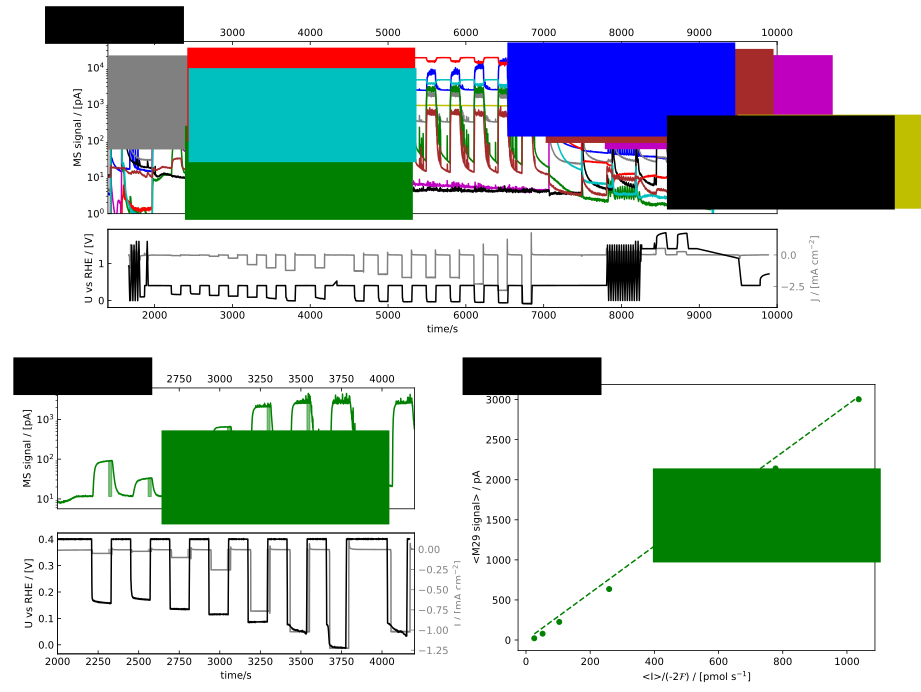
\includegraphics[width=1\textwidth]{02_Tools/fig/internal_calibrations_2.png}
	\caption{Calibration experiment for propane (\ch{C3H8}) by reduction (hydrogenation) of propene (\ch{C3H6}) on Pt in 1.0 M \ch{HClO4}. \textbf{(a)} The entire experimental dataset, taken immediately after that in Figure \ref{fig:internals}a. \textbf{(b)}, A zoom-in is shown for the propane calibration. The data points at larger current, where propene reduction is mass-transport limited and some of the current goes to HER are excluded. \textbf{(c)}, The resulting calibration curve is plotted as near-steady-state signal vs production rate.
	}
	\label{fig:internals_2}
\end{figure}
Once a sensitivity factor $F_M^i$ is determined, it can be used to calculate the flux of $i$ from the signal at $M$ according to:
\begin{equation}
\dot{n}^i_{\text{vac}} = \frac{1}{F_M^i} S_M = C_M^i S_M\,,
\end{equation}
where $C_M^i$ is a \textit{calibration factor}, which in this simple case is just the reciprocal of the sensitivity factor.

Figure \ref{fig:internals_2} shows a calibration for an additional reaction that can be run at 100\% Faradaic efficiency on platinum: the propene reduction reaction, Reaction \ref{rxn:PRR}:
\begin{equation}
\ch{C3H6 + 2 (H+ + e- ) -> C3H8}\label{rxn:PRR}
\end{equation}
I first encountered this reaction while doing the propene striping experiments reported in Paper \ref{Winiwarter2019}. Briefly, we found that the tendency of adsorbed propene to strip off from a palladium surface as propane or propene on a cathodic sweep correlates with the coverage on the surface, motivating a mechanism for the propene oxidation reaction (the main subject of that paper) in which surface coverage guides the reaction pathway towards certain intermediates.  This is, in my opinion, a fantastic story, and was a great project to be part of, though it is out of the scope of this Thesis. I highly recommend the paper to an interested reader of this Thesis. Anna Winiwarter has since expanded on those EC-MS experiments to probe propene reactivity. However, propene reduction is included here only because it demonstrates well some of the challenges and opportunities in quantitative EC-MS.

The first challenge in quantification of propane and propene is that there is a significant overlap in their mass spectra (Figure \ref{fig:spectra}). Propane can itself be detected and quantified without interference at its most prominent mass fragment, m/z=29. The sensitivity factor of propane at m/z=29, $F_{\text{M29}}^{\ch{C3H8}}$, is determined by Faradaic propene reduction in Figure \ref{fig:internals_2}b and c. 
\begin{figure}[t]
	\centering
	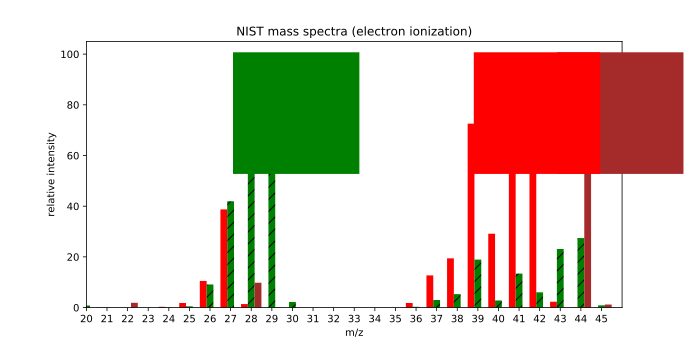
\includegraphics[width=0.8\textwidth]{02_Tools/fig/mass_spectra.png}
	\caption{Mass spectra of propene (\ch{C3H6}, red), propane (\ch{C3H8}, green and hatched), and \ch{CO2} (brown) from NIST\cite{NIST}
	}
	\label{fig:spectra}
\end{figure}
However, propane interferes with two other molecules of interest at their most prominent mass fragments: propene at m/z=41 and \ch{CO2} at m/z=44.

To deal with this, using \ch{CO2} as an example: In situations where both propane and \ch{CO2} are present, we should subtract the portion of the m/z=44 signal which is due to propane before dividing by $F_\text{M44}^{\ch{CO2}}$ to get the \ch{CO2} flux. The m/z=44 signal which is due to propane can, in turn, be calculated from the m/z=29 signal, which is solely due to propane. Mathematically,
\begin{align}
\dot{n}^{\ch{CO2}}_{\text{vac}} &= \frac{1}{F^{\ch{CO2}}_\text{M44}}S^{\ch{CO2}}_\text{M44}\\
&= \frac{1}{F^{\ch{CO2}}_\text{M44}}\left(
S_\text{M44} - S^{\ch{C3H8}}_\text{M44}
\right)\\
&= \frac{1}{F^{\ch{CO2}}_\text{M44}}\left(
S_\text{M44} - \frac{I^{\ch{C3H8}}_\text{M44}}{I^{\ch{C3H8}}_\text{M29}}S^{\ch{C3H8}}_\text{M29}
\right)\\
&= \frac{1}{F^{\ch{CO2}}_\text{M44}}S_\text{M44} - \frac{I^{\ch{C3H8}}_\text{M44}}{F^{\ch{CO2}}_\text{M44}I^{\ch{C3H8}}_\text{M29}}S_\text{M29}\,,
\end{align}
where $I_M^i$ is the relative intensity at m/z=$M$ for in the mass spectrom of analyte $i$. These are taken from NIST. 

The substitution of $S_\text{M29}$ for $S^{\ch{C3H8}}_\text{M29}$ assumes that all of the signal at m/z=29 is due to propane.

Another way to write this is 
\begin{align}
\dot{n}^{\ch{CO2}}_{\text{vac}} = C_\text{M44}^{\ch{CO2}} S_\text{M44} + C_\text{M29}^{\ch{CO2}} S_\text{M29}
\,\hspace{5mm}\text{with}\\
C_\text{M44}^{\ch{CO2}} = \frac{1}{F_\text{M44}^{\ch{CO2}}}\hspace{5mm}\text{and}\hspace{5mm} C_\text{M29}^{\ch{CO2}} = - \frac{I^{\ch{C3H8}}_\text{M44}}{F^{\ch{CO2}}_\text{M44}I^{\ch{C3H8}}_\text{M29}}
\end{align} 
In general, we can write 
\begin{align}
\dot{n}^{i}_{\text{vac}} = \sum_M C_M^i S_M\,,
\end{align}
or, in vector form
\footnote{
The \texttt{Molecule} class of the \texttt{EC\_MS} python package (Appendix \ref{app:EC_MS}) implements both the simple ($F_M^i$) and vectorized ($\mathbf{C}^i$) quantification techniques presented above. Fortunately, it is for only a few projects that I've had to use the vectorized approach, and this does not include any of the isotope-labeling studies presented later in this Thesis.
}:
\begin{align}
\dot{n}^{i}_{\text{vac}} = \mathbf{C}^i \cdot \mathbf{S}
\end{align}




\subsection{External calibration based on the capillary flux}\label{subsec:capillary}

The determination of the sensitivity factors $F_M^i$ by Faradaic production of analyte $i$ described in the previous Subsection is referred to as \textit{internal calibration}, since all of the molecules giving the signal in the calibration experiment are made inside the working volume of the EC-MS setup, and the amount of analyte is known. Here, we describe \textit{external calibration}, whereby a carrier gas, originating outside the setup (in a bottle, or, in the case of air, from the room), is leaked through the capillary of the chip and into the mass spectrometer. The challenge then, in determining the sensitivity factor $F_M^i$ to enable quantification by Definition \ref{d:quantification}, is to determine the flux through the capillary of analyte $i$ given the composition of the gas in the chip. In other words, it is to determine the \textit{capillary flux}. 

The flow of molecules through the capillary goes through at least three regimes as the pressure drops from 1 bar to high vacuum\cite{Henriksen2009}: (1) a viscous flow regime near ambient pressure, (2) a transition regime, and (3) a molecular flow regime governed by Kundsen diffusion near high vacuum. It is therefore not trivial to derive an analytical expression, but this has been done. It is\cite{Trimarco2017_PhD}:
\begin{equation}
\dot{n}_{\mathrm{cap}} = \frac{1}{R T}\frac{1}{l_\text{cap}} 
\left(\left( 
\frac{\pi}{8\nu}a^4\bar{p} + \frac{2\pi}{3}a^3\bar{v} \frac {1+2\frac{2\sqrt{2}}{\sqrt{\pi}}\frac{a}{\eta}\frac{\bar{p}}{\bar{v}}} {1+2.48\frac{2\sqrt{2}}{\sqrt{\pi}}\frac{a}{\eta}\frac{\bar{p}}{\bar{v}}}
\right)
\left(p_1-p_{\mathrm{tran}}\right) 
+ 
\frac{2\pi}{3}a^3\bar{v}\left(p_{\mathrm{tran}}-p_2\right)\right) 
\;, \label{eq:capillary}
\end{equation}
Here, $p_1$ is the inlet pressure (usually 1 bar), $p_2$ is the outlet pressure ($\approx$ 0), $p_{\mathrm{tran}}=\frac{k_B T}{2 \sqrt{2}\pi s^2 a}$ is the pressure at which the transition from viscous to molecular flow occurs, $\bar{p}=\frac{p_1 + \bar{p}_{\mathrm{tran}}}{2}$ is the average pressure in the viscous flow regime, $\eta$ is the viscosity of the gas, $s$ is the molecular diameter, $\bar{v}=\sqrt{\frac{8 k_B T}{\pi m}}$ is the mean thermal velocity of the gas molecules, and $m$ is the molecular mass. Furthermore, $l_\text{cap}$ is the length of the capillary, and $a=h_\text{cap}=w_\text{cap}$ is its height and width, assumed to be equal (square cross-section). By design, $l_\text{cap} = 1\,\text{mm}$, $w_\text{cap} = 6\,\mu\text{m}$, and $h_\text{cap} = 6\,\mu\text{m}$.

This equation has been validated experimentally for a microreactor by sealing the outlets of an interface block and measuring the rate at which the pressure dropped as air leaked through the chip's capillary into the vacuum chamber\cite{Henriksen2009}.

With the internal calibration described in the previous Subsection, however, there is an easier and more precise way to validate the capillary flux: compare the signal due to a molecule in the carrier gas to the signal when the same molecule is produced electrochemically. This is most easily, done for \ch{O2}, as \ch{O2} can be produced electrochemically with near-100\% Faradaic efficiency, and is also present in air, giving a ``free'' carrier gas measurement.

In the dataset presented in the previous Subsection, an air measurement is provided at the very beginning (i.e. t$\approx$ 1500 s) of Figure \ref{fig:internals_2}. Here, the m/z=32 signal is 1.88$\cdot 10^{-9}$ A. The corresponding \ch{O2} flux, based on the sensitivity factor $F$ calibrated internally, is
\begin{equation}
\dot{n}^{\ch{O2}}_\text{cap} = \frac{S_\text{M32}}{F^{\ch{O2}}_\text{M32}} = \frac{1.88\cdot 10^{-9} \text{[A]}}{1.11 \left[\frac{\text{C}}{\text{mol}}\right]} = 1.70 \left[\frac{\text{nmol}}{\text{s}}\right]
\end{equation}
Using the value of $x^{\ch{O2}}_\text{air}=20.95$\% for the \ch{O2} content of air and assuming that there is not significant separation effect on the gases in air by the capillary, the capillary flux of air is 
\begin{equation}
\dot{n}^{\text{air}}_\text{cap} = \frac{\dot{n}^{\ch{O2}}_\text{cap}}{x^{\ch{O2}}_\text{air}} = 8.08 \left[\frac{\text{nmol}}{\text{s}}\right]\,.
\end{equation}
In contrast, the flux of air through the capillary predicted by Equation \ref{eq:capillary}, using the design parameters for $l_\text{cap}$, $h_\text{cap}$, and $w_\text{cap}$, is 6.86 nmol/s. How do reconcile this difference? In reality, it is $h_\text{cap}$ which varies from capillary to capillary. This is a result of non-uniformity in the etching step that forms the capillary\cite{Trimarco2017_PhD}. The actual capillary height, as measured by profilometry in the clean room, can vary by $\approx$ 20 \% across a wafer, which leads to varying permeability, and thus varying air flux. 

In fact, calibrating the \ch{O2} signal at m/z=32, and then measuring the m/z=32 signal in air is a way to \textit{calibrate the chip capillary}. Since the real variation in the capillary flux is due to variation in the capillary height, the most correct way to account for it would be to solve Equation \ref{eq:capillary} for $h_\text{cap}$ with the measured $\dot{n}_\text{cap}^\text{air}$. However, in practice (so far), to make the implementation easier, we incorporate the difference in an effective capillary length:
\begin{equation}
l_\text{eff} = \frac{\dot{n}^{\text{air}}_\text{cap, pred.}}{\dot{n}^{\text{air}}_\text{cap, meas.}} l_\text{cap}= \frac{6.86 \left[\frac{\text{nmol}}{\text{s}}\right]}{8.08 \left[\frac{\text{nmol}}{\text{s}}\right]} 1.00\,\text{[mm]} = 0.85\,\text{[mm]}
\end{equation}
If $l_\text{eff}$ is used instead of $\l_\text{cap}$ for in Equation \ref{eq:capillary}, the equation predicts the ``correct'' value for the flux of air, i.e. the measured flux as calibrated by OER. 

With the chip thus calibrated, we can use Equation \ref{eq:capillary} with $l_\text{eff}$ to calculate the capillary flux of any gas $i$, given its dynamic viscosity $\eta^i$, molecular diameter $s^i$, and molecular mass $m^i$. All that is then needed is a mass spectrometer signal at an m/z=$M$ without interference using $i$ as a carrier gas, and we can calculate its sensitivity factor $F_M^i$. The datasets presented in Figures \ref{fig:internals}a and \ref{fig:internals_2}a include the necessary data for such external calibration of several gases. The results are shown in Table \ref{tab:externals}. When possible, the sensitivity factor determined by electrochemistry is included for comparison. While the internal and external calibrations for \ch{O2} in air match by the definition of $l_\text{eff}$, the agreement for \ch{H2} and \ch{CO2} is also quite good, validating the method.

\begin{table}
	\centering
	\resizebox{\textwidth}{!}{%
	\begin{tabular}{c|c|c|c|c|c||c|c|c|c||c}
		Molecule & $\eta$ & $s$ & $m$ & $x^i$ & $\dot{n}_\text{cap}^i$ & dataset & time & m/z=$M$ & $F_M^i$ & $F_M^i$ (EC) \\
		& / [$\mu$Pa$\cdot$s] & / [\AA] & / [amu]& & / [nmol/s] & & / [s]& & / [C/mol] & / [C/mol] \Bstrut\\
		\hline
		\ch{O2} in air & 18.5 & 3.66 & 30.0 & 0.2095 & 1.70 & 
		 \ref{fig:internals_2}a & 1525 & 32 & 1.11 & 1.11 \Tstrut\\
		\ch{N2} in air & 18.5 & 3.66 & 30.0 & 0.7808 & 6.33 & 
		 \ref{fig:internals_2}a & 1525 & 28 & 1.42 & - \\
		\ch{Ar} in air & 18.5 & 3.66 & 30.0 & 0.0093 & 0.0755 & 
		 \ref{fig:internals_2}a & 1525 & 40 & 0.98 & - \\
		\ch{He} & 20.0 & 2.15 & 4.0 & 1 & 8.64 & 
		 \ref{fig:internals}a & 10400 & 4 & 0.71 & - \\
		\ch{CO} & 17.8 & 3.76 & 28.0 & 1 & 7.14 & 
		 \ref{fig:internals}a & 5000 & 28 & 1.24 & - \\
		\ch{H2} & 8.9 & 2.71 & 2.0 & 1 & 16.50 & 
		 \ref{fig:internals}a & 7200 & 2 & 1.83 & 1.81 \\
		\ch{O2} & 20.7 & 3.55 & 32.0 & 1 & 6.24 & 
		 \ref{fig:internals}a & 10900 & 32 & 1.04 & 1.11 \\
		\ch{CO2} & 15.0 & 4.53 & 44.0 & 1 & 9.38 & 
		 \ref{fig:internals_2}a & 9850 & 44 & 1.32 & 1.23 \\
		\ch{C3H6} & 8.85 & 4.50 & 42.1 & 1& 15.11 & 
		 \ref{fig:internals_2}a & 4400 & 41 & 1.22 & - \\
	\normalsize
	\end{tabular}
	}
\caption{External calibrations. The flow properties of the carrier gas $\eta$, $s$, and $m$ as well as the fraction $x^i$ of component $i$ are used to calculate the flux of $i$ through the capillary, $\dot{n}^i_\text{cap}$. This is compared to the measured signal at a given m/z in a given dataset, where the dataset refers to Figure \ref{fig:internals} or \ref{fig:internals_2} of the previous Subsection. Dataset \ref{fig:internals} was taken with a chip with $l_\text{eff}=0.99$ mm and Dataset \ref{fig:internals_2} was taken with a chip wtih $l_\text{eff}=0.86$ mm, $l_\text{eff}$ being used to calculate $\dot{n}^i_\text{cap}$. The signal at m/z=$M$ was averaged over 50 s centered at the time indicated, chosen for a steady interference-free measurement. The sensitivity factor $F_M^i$ is the ratio of that signal to $\dot{n}_\text{cap}^i$. This is compared, when possible, to $F_M^i$ calculated by electrochemical (internal) calibration.
}
\label{tab:externals}
\end{table}



\subsection{Sensitivity factors from theory, and non-ideal effects}\label{subsec:MS_theory}

The \textit{internal} and \textit{external} calibration methods described above, linked via $l_\text{eff}$, enable the determination of sensitivity factors for any analyte which can either be produced electrochemically with 100\% Faradaic efficiency or flowed through the chip as a carrier gas. However, these conditions often exclude analytes of interest. If sensitivity factors could be \textit{predicted} through first principles, then any analyte could be quantified. In this Subsection, I propose such a method and check its ability to predict the variation in the sensitivity factors determined in the previous two Subsections.

It is hard to find anything in the literature about predicting mass spectrometry sensitivity from first principles, not least because applications requiring quantification as understood by Definition \ref{d:quantification} are quite rare. The following steps happen between a molecule $i$ entering the vacuum chamber and a signal at m/z=$M$ being registered (Figure \ref{fig:MS})\cite{Gross2007}:
\begin{itemize}
	\item
	The molecule must reach the filament
	\item
	The molecule must be ionized by the filament
	\item
	The ionization must result in a fragment at m/z=$M$
	\item
	The fragment must be transmitted through the quadrupole while it is filtering for m/z=$M$
	\item
	The fragment starts an electron cascade on the secondary electron multiplier (SEM)
\end{itemize}
The signal $S_M$ (in A) can thus in principle be related to the flux $\dot{n}^i_\text{vac}$ by a series of probibilites $P$ and the SEM amplification $A$:
\begin{equation}
S_M = \dot{n}^i_\text{vac} P_\text{filament} P_\text{ionize}(i) P_\text{fragment}(i, M) P_\text{transmission}(M) A(M)\,,
\end{equation}
Where I've tried to indicate whether each probability depends on the identity of the molecule $i$ or the mass of the fragment $M$.

The probability of reaching the filament $P_\text{filament}$ depends a lot on the geometry of the vacuum chamber, notably where the inlet, filament, and pump are in relation to each other. I'll assume that it doesn't depend on $i$ or $M$. The ionization probability $P_\text{ionization}(i)$ is proportional to the ionization cross section $\sigma^i$ of analyte $i$, which is generally available in the literature. It depends on the ionization energy, which is 70 eV for all of the work in this PhD thesis. The probability of a given fragment being formed after the molecule is ionized can be calculated from the mass spectrum:
\begin{equation}
P_\text{fragment}(i, M) = \frac{I_M^i}{\sum_{M'}I_{M'}^i}
\end{equation}
where $I_{M'}^i$ is the intensity of mass fragment $M'$ in the electron ionization mass spectrum of analyte $i$. These mass spectra, which also depend on the ionization energy, are often available at NIST\cite{NIST}. They can also be measured directly in the EC-MS setup if $i$ is available as a carrier gas. 

The processes after fragmentation can be assumed to only depend on the fragment mass-to-charge ratio $M$. Both of these processes, quadrupole transmission and SEM amplication factor, will also depend on the ion acceleration. They can be grouped into a function $T(M)$ which I will refer to as the \textit{transmission function}, implying that the transmission through the quadrupole is gives most of the mass dependence, even though I'm not sure this is true.

\begin{figure}[t]
	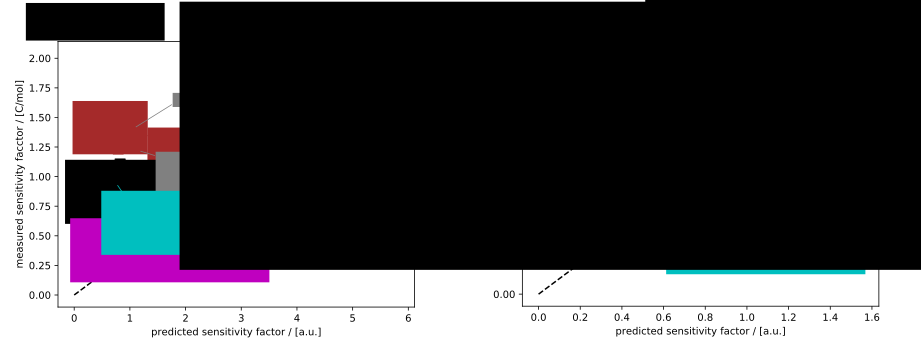
\includegraphics[width=\textwidth]{02_Tools/fig/calibration_results.png}
	\caption{Measured sensitivity factor $F_M^i$ vs predicted sensitivity factor $f_M^i$ for two guesses at the transmission function: \textbf{(a)}, inversely proportional with the m/z ratio; and \textbf{(b)}, inversely proportional with the square root of the m/z ratio. The measured sensitivity factors, which are shown in Table \ref{tab:externals}, are determined via capillary flux (triangles) or an electrochemical reaction (squares). }
	\label{fig:transmission}
\end{figure}

Overall, then, the predicted sensitivity factor, which is denoted with a little $f$ to distinguish it from the experimentally determined big $F$, is
\begin{equation}
f_M^i = \frac{S_M}{\dot{n}^i_\text{vac}} = k \sigma_i \frac{I_M^i}{\sum_{M'}I_{M'}^i} T(M)\,.\label{eq:rsf}
\end{equation} 
Where $k$ is a proportionality factor, which I choose to set $f_{\text{M28}}^{\ch{N2}} = 1$. The challenge, then, is to determine $T(M)$.

Some hints can be found from quadrupole theory\cite{Douglas2009}: For a quadrupole mass analyzer, the transmission function should correlate inversely with the resolution $R = M / \Delta M$. A perfectly-tuned mass spectrometer should have a constant mass resolution resolution, i.e. $\Delta M = c$. If so, the resolution varies directly with $M$. This implies that the transmission function should vary inversely with $M$, i.e., $T(M)=M^{-1}$.

Figure \ref{fig:transmission}a shows the measured $F_M^i$ plotted against the thus-calculated $f_M^i$ with $T(M)=M^{-1}$. The predictive scheme does a terrible job at explaining the variation in the data.

If we keep the form of the transmission function and change the exponent, we can get a relatively good fit by putting the exponent to -1/2. This may indicate that the SEM amplication factor scales with $M^{+1/2}$, or may indicate that the above reasoning doesn't quite hold. In any case, 
\begin{equation}
T(M)=M^{-\frac{1}{2}}
\end{equation}
seems to give a good fit. The best-fit line of proportionality between $F$ and $f$ gives a root-mean-square error on the prediction of $F$ of 12\%. In other words, we can quantify an arbitrary new analyte $i$ at mass $M$ to within about 12\% accuracy (25\% within two standard deviations) without a new calibration. We have developed a generalized solution to the problem of quantification as understood by Definition \ref{d:quantification}!
\vspace{5mm}

There is, however, an important exception: if the carrier gas influences the sensitivity of the mass spectrometer, then all bets are off. This actually seems to be the case when propene is the carrier gas. Figure \ref{fig:internals_2} shows an internal calibration for propane by propene reduction. In the higher-current steps in Figure \ref{fig:internals_2}a, propene reduction is mass-transport limited and hydrogen is also produced. Assuming that there are no Faradaic processes other than propene reduction to propane and hydrogen evolution, the amount of hydrogen produced can be determined from the electrode current and the calibrated propane signal. Figure \ref{fig:propene_transmission}a shows the data used to test the \ch{H2} calibration in propene, calibrated using the \ch{H2} sensitivity factor calculated in He. Faradaic analysis shows that the \ch{H2} signal is consistently $\approx 3$ times larger than expected based on subtracting the calibrated propane signal from the total current density, and using the calibration of \ch{H2} at m/z=2 by HER in He carrier gas. This implies that the sensitivity factor of \ch{H2} at m/z=32 ($F_\text{M2}^{\ch{H2}}$) with propene as the carrier gas is $\approx 3$ times larger than it is with He as a carrier gas. The sensitivity factors for \ch{H2} at m/z=2 and for propane at m/z=29 are included, versus the sensitivity factors predicted by Equation \ref{eq:rsf} with $T(M)=M^{-1/2}$, in Figure \ref{fig:propene_transmission}b. They are both way above the trendline set by the calibration factors measured in other carrier gases.
\begin{figure}[b!]
	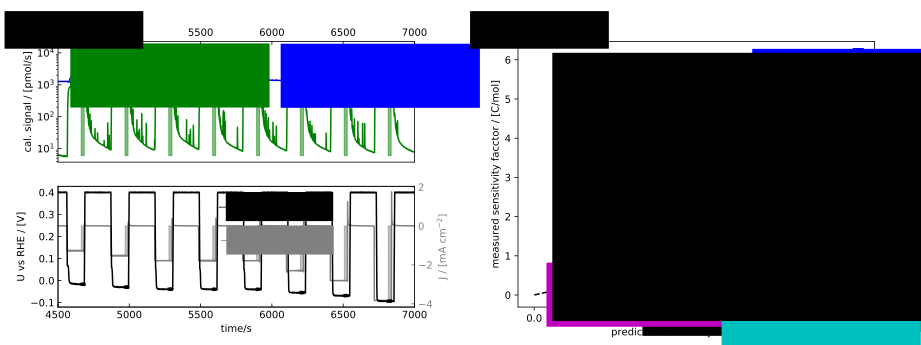
\includegraphics[width=\textwidth]{02_Tools/fig/H2_in_propene_experiment.png}
	\caption{Non-ideality with propene as carrier gas: \textbf{(a)}, Propene reduction + HER, data from Figure \ref{fig:internals_2}a. \textbf{(b)}, Measured vs predicted calibration factors including propane at m/z=29 measured by propene reduction and \ch{H2} at m/z=2 measured by HER in propene, which do not fit the trend of the other masses. A transimission function of $T(M) = M^{-1/2}$ was used for the predicted calibration factor. Propene was measured at m/z=41 and propane at m/z=29. The others analytes are measured at the same masses as in Figure \ref{fig:transmission}. The green dot shows the prediction for the sensitivity factor of propane at m/z=29.}
	\label{fig:propene_transmission}
\end{figure}

These unpredictable and therefore undesireable effects of propene on the mass spectrometer sensitivities are likely due to space-charge effects. Propene has the highest capillary flux of the carrier gases used (Table \ref{tab:externals}) due to its low viscosity, and has a rather high ionization cross-section. This results in a high concentration of ions in the mass spectrometer, which apparently leads to generally increased sensitivity, though I do not claim to understand why. Nonetheless, the response at m/z=29 is linear with propane production rate (Figure \ref{fig:internals_2}c), indicating that quantification of propane using this sensitivity factor is valid when propene is the carrier gas.

The question is then: 
\begin{question} 
	How should we quantify propane in a carrier gas other than propene?
\end{question}
This is, in fact, what we wished to do for the propene stripping experiments in Paper \ref{Winiwarter2019}, where the interesting signal is the propane that comes off in inert gas after propene has been adsorbed on the surface. I think the best strategy is to predict the sensitivity factor for propane in He based on the other calibrations and the trendline in Figure \ref{fig:transmission}b. This prediction is indicated by the green dot in Figure \ref{fig:propene_transmission}b. Whereas propene reduction to propane gives a sensitivity factor of $F^{\ch{C3H8}}_\text{M29} = 2.93$ C/mol, the theory presented in this Subsection indicates the calibration factor in He is $F^{\ch{C3H8}}_\text{M29} = 1.3$ C/mol (to within $\approx$ 25\%). We had not yet understood this effect of propene on the overall sensitivity of the mass spectrometer when publishing Paper \ref{Winiwarter2019}, and thus likely underestimated the amount of propane desorbed in the striping experiments reported there by a factor of $\approx 2$.


\subsection{Quantitative mass spectrometry in practice - methanol synthesis and CO reduction}\label{subsec:in_practice}

The aim of this Subsection is to provide practical suggestions on how to use the calibration methods described in the previous Subsections for users of EC-MS and other techniques benefiting from quantification as understood by Definition \ref{d:quantification}. Let's say you want to quantify a gaseous analyte $i$. First you need to find a mass-to-charge ratio $M$ at which no other molecules in your experiments will give a signal, or at least where you expect the interference to be manageable (as described in the end of Subsection \ref{subsec:internal}). The goal then is to determine the sensitivity factor $F_M^i = S_M/\dot{n}^i_\text{vac}$. You have three options, none of which excludes the others:
\begin{enumerate}
\item 
\textit{Internal calibration}
\footnote{Internal calibration is implemented with the function \texttt{calibration\_curve} of the \texttt{EC\_MS} python package (Appendix \ref{app:EC_MS}). This function also produces plots of the types in Figure \ref{fig:internals}b-e.}
, Subsection \ref{subsec:internal}:

If you can produce a known number of molecules of your analyte by an electrochemical reaction, then do so, and measure the signal! This is the most certain way to get a sensitivity factor, as it relies on no assumptions other than Faraday's law of electrolysis (Equation \ref{eq:Far}) to determine $\dot{n}^i_\text{el}$, which is equal to $\dot{n}^i_\text{vac}$ at steady-state or when integrated. A drawback is if a reactant gas is needed which won't be the carrier gas during the measurements you wish to quantify, since in some cases the carrier gas can influence the sensitivity factors. Furthermore, knowing how many molecules you produced generally requires being able to assume 100\% Faradaic efficiency. In my experience, there is often a small but constant amount of residual current from some other process, so internal calibration should use several different current densities and use the slope of the line-of-best-fit between the measured $S_M$ and expected $\dot{n}^i_\text{el}$ as the sensitivity factor.

\item 
\textit{External calibration}
\footnote{External calibration is implemented with the function \texttt{point\_calibration} of the \texttt{EC\_MS} python package.}
, Subsection \ref{subsec:capillary}:

If you have $i$ available as a gas, either pure or diluted, then you can fill the chip with this gas and measure the signal at $M$. However, this requires that you know the capillary flux through the chip. The capillary flux can be calculated by Equation \ref{eq:capillary}, but only if the capillary dimensions are known, and in practice these dimensions vary a bit from chip to chip. Thus, external calibration requires a \textit{chip calibration}.
\begin{itemize}
	\item \textit{Chip calibration}
	\footnote{Chip calibration is implemented with the function \texttt{chip\_calibration} of the \texttt{EC\_MS} python package.}
	, Subsection \ref{subsec:capillary}:
	
	A chip calibration means determining the effective capillary length $l_\text{eff}$ that can take the place of $l_\text{cap}$ in Equation \ref{eq:capillary} so that it predicts the measured flux of an analyte with a sensitivity factor determined by internal calibration. Typically, this means determining $F_\text{M32}^{\ch{O2}}$ using OER, and then measuring the m/z=32 signal while the chip is open to air.
\end{itemize}
\item 
\textit{Predictive calibration}
\footnote{Predictive calibration is implemented with the function \texttt{recalibrate} of the \texttt{EC\_MS} python package (Appendix \ref{app:EC_MS}). This function also produces plots of the type in Figure \ref{fig:transmission}.}
, Subsection \ref{subsec:MS_theory}:

If a number of other sensitivity factors, $F_{N}^{j}$, can be obtained by internal or external calibration, then these other sensitivity factors can be used to predict $F_M^i$. A predicted calibration $f_N^j$ is calculated for each other molecule $j$ according to Equation \ref{eq:rsf}. This requires knowledge of the ionization cross-sections and mass spectra of all the analytes (available in the literature, usually at NIST\cite{NIST}) and a \textit{transmission function} $T(M)=M^x$ describing the dependence of the sensitivity on the mass fragment. $T(M)$ depends on the tuning of the mass spectrum, and at the setup used for this PhD project, $T(M)=M^{-1/2}$ works well. As many internal and external calibrations as possible should be used to fit and build confidence in $T(M)$. Once a line of proportionality $F_N^j = a f_N^j$ is established, $F_M^i$ is predicted by calculating $f_M^i$ by Equation \ref{eq:rsf} and multiplying by $a$.
\end{enumerate}

Ideally, at the start of a research project, all three of the above strategies should be used for as many analytes of interest as possible. Plotting $F$ against $f$ will help find non-ideal effects such as that described for propene as a carrier gas in Subsection \ref{subsec:MS_theory}.

Notice that predictive calibration relies on calibrating as many molecules as possible by external calibration or internal calibration in order to determine $T(M)$ and the proportionality between $F$ and $f$. Note also that external calibration depends on a chip calibration which in turn depends on an internal calibration. And internal calibration relies on using the current for an electrochemical reaction to know the flux of a molecule to the vacuum chamber. Thus: \textbf{Robust quantification as meant in Definition \ref{d:quantification} is made possible by the coupling of electrochemistry and mass spectrometry}.

This quantification platform can, however, be extended to applications that do not involve electrochemistry. As an example, my colleague Alexander Krabbe is doing a project on methanol synthesis catalysts. As such, he is interested in measuring the TOF for methanol synthesis in a thermal microreactor setup. This means determining the flux of methanol to the vacuum chamber $\dot{n}_\text{vac}^{\ch{CH3OH}}$ from the signal at its most pronounced mass fragment $S_\text{M31}$. This means determining $F_\text{M31}^{\ch{CH3OH}}$. The problem is especially challenging since methanol, being a liquid at room temperature, is not available as a carrier gas. We developed the following procedure:
\begin{enumerate}
	\item Determine $F_\text{M32}^{\ch{O2}}$ on the EC-MS setup by internal calibration using OER. \label{step:meth1}
	
	\item Use $F_\text{M32}^{\ch{O2}}$ on the EC-MS setup to determine the flux of air through the capillary of an EC-MS membrane chip, and thus $l_\text{eff}$ (chip calibration). 
	
	\item Install the calibrated membrane chip on the microreactor setup. Since the flux of \ch{O2} through the membrane chip's capillary $\dot{n}_\text{vac}^{\ch{O2}}$ is known, measuring the m/z=32 signal gives $F_\text{M32}^{\ch{O2}}$ for the \textit{microreactor setup}!
	
	\item Install a microreactor on the microreactor setup, and fill it with 1 bar \ch{O2}. Since $F_\text{M32}^{\ch{O2}}$ for the microreactor setup is known, the $S_\text{M32}$ signal tells us the \ch{O2} flux through the microreactor's capillary, and thus its $l_\text{eff}$. We now have a \textit{chip calibration of the microreactor}. \label{step:meth4}
	
	\item Use the calibrated microreactor for external calibrations on the microreactor setup: Flow a number of carrier gases spanning a range of molecular masses, viscosities, and ionization cross-sections through the microreactor, f. eks. \ch{He}, \ch{H2}, \ch{O2}, \ch{Ar}, \ch{CH4}, \ch{CO2}, etc. Use the signal at the most intense mass fragment and the calculated flux with $l_\text{eff}$ to determine a sensitivity factor $F$ for each of the gases.
	
	\item Determine the transmission function $T(M)$ that gives the best fit to a line of proportionality between the measured sensitivity factors ($F$) determined by external calibration and the predicted sensitivity factors ($f$) calculated for each of the gases. Then determine $F_\text{M31}^{\ch{CH3OH}}$ with predictive calculation, by calculating $f_\text{M31}^{\ch{CH3OH}}$ and multiplying by the proportionality constant.
\end{enumerate} The functions of \texttt{EC\_MS} do each step of the data analysis and calculations, making the whole procedure described above quite quick and painless. Furthermore, steps 1 through 4 need only be done once, so long as the microreactor with the calibrated capillary flux is not lost or damaged. (It just so happens that EC-MS membrane chips can go on the microreactor setup but not vice versa, or this procedure could be a step shorter.)
\begin{figure}[t]
	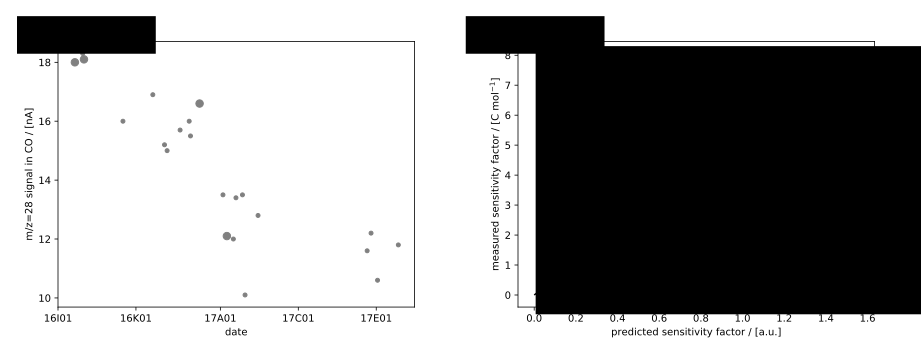
\includegraphics[width=\textwidth]{02_Tools/fig/calibration_results_sniffer2.png}
	\caption{\textbf{(a)}, Signal at m/z=28 with 1 bar \ch{CO} in the membrane chip as carrier gas for experiments done over a period from September 2016 to May 2017. The date on the x-axis is written as \texttt{yyMdd} with \texttt{M}=A representing January, B representing February, etc. \textbf{(b)}, Internal, external, and predicted calibrations for the dataset used in Paper \ref{Trimarco2018}. This is a correction to Figure S6b from the SI of that paper.}
	\label{fig:CuNPs}
\end{figure}

This leads us to the question:
\begin{question}
	How often should one calibrate?
\end{question}
 Figure \ref{fig:CuNPs}a helps answer the question.

This figure includes one data point for each ``successful'' experiment (meaning nothing broke before starting the measurement, results or lack thereof aside - the setup was still under development) during a project on CO reduction that took up most of the first year of my PhD and which we put on hold due to difficulties with reproducibility
\footnote{In that project, which is out of the scope of this Thesis and is, at present, best described in the PhD theses of Anders Bodin\cite{Bodin2017_PhD} and Daniel Trimarco\cite{Trimarco2017_PhD}, we used the EC-MS setup to measure transient phenomena during \ch{CO} reduction on mass-selected, vacuum synthesized copper nanoparticles. Briefly: we drafted an article, included in the appendix to both of those PhD theses, describing how the copper nanoparticles show a transient high selectivity for methane production during the first few seconds of applied potential, whereas ethylene selectivity is more steady. Furthermore, we showed that this methane transient has an independent Tafel slope and depends on prior exposure to air-saturated electrolyte, indicating that oxygen activates the catalytic surface towards a reaction pathway not normally accessible. This was of high interest due to the heated debate in the literature about the effect of oxygen on copper's \ch{CO2} and \ch{CO} reduction activity\cite{Mistry2016, Gao2017a, Eilert2017, Nitopi2019} (see also, for example, Paper \ref{Scott2019_GIXRD}). We never ended up submitting the draft though, because out of tens of measurements, we were only able to reproduce the result a handful of times (the big dots in Figure \ref{fig:CuNPs}a), with the other experiments showing CO reduction activity not significantly higher than the blank glassy carbon substrate; and we could never see the copper on the sample after the experiment, indicating the nanoparticles were not stable. The work is ongoing, now led by Jakob Ejler, Degenhart Hochfilzer and Ezra Clark. Getting reproducible results on the mass-selected copper nanoparticles is still remarkably challenging, but they are making progress with a patient, systematic approach - in contrast to the brute-force approach that Daniel, Anders, and I had started out with.}
.
Figure \ref{fig:CuNPs} was one of my many unsuccessful attempts to find something, ideally within our control, that could separate the ``good results'' from the bad: it shows the m/z=28 signal from the CO carrier gas at the same time during each of those experiments. Unfortunately, it didn't help at all in figuring out what kept going wrong, but it does shed light on the nature of the variability which quantitative mass spectrometry is up against.

Since all of the measurements were made with the same pressure of \ch{CO} flowing through the capillary of chips from the same batch to the same mass spectrometer (which we of course did not tune in the middle of the project), all of the m/z=28 signals should in principle be identical. However, there is both a scatter of +/- approximately 10\% and a gradual drift with a signal loss on the order of 45\% over nine months. The scatter is probably mostly due to the variation in the actual chip capillary dimensions (we were breaking chips quite frequently during that project), but we can't rule out sensitivity effects related to the recent history of the mass spectrometer. The drift is likely due to the mass spectrometer gradually falling out of tune. 

The scatter indicates that it is best to have a calibration on the same day as the measurement. However, calibration of one molecule should be enough, assuming that it is the absolute sensitivity that drifts and not the relative sensitivity. This can be done by internal calibration of one molecule (for example \ch{H2} by HER, which is the inert-gas activity test often used for comparison anyway when studying CO or \ch{CO2} reduciton), or just by measurement of the signal of air or a carrier gas if $l_\text{eff}$ is known for the chip. If an external calibration is used for this purpose, each new chip has to be calibrated - meaning an air measurement through the chip and an OER measurement on the same day (though not necessarily the day of the experiment to be quantified).

The harder work is at the beginning of a project, or if the mass spectrometer is tuned: At that time, make a plot of the type in Figure \ref{fig:CuNPs}b with as many internal and external calibrations as possible. This determines $T(M)$ in case any sensitivity factors need to be predicted in the absence of an internal or external calibration, and gives the relative sensitivities of all the molecules of interest. Then, scale these up or down according to one calibration taken on the day of the measurement.
\footnote{This procedure is facilitated by the \texttt{save\_calibration\_results} and \texttt{load\_calibration\_results} functions of the \texttt{EC\_MS} python package.} 
Of course when there is only one analyte of quantitative interest - for example in OER studies - a simple calibration can be done each measurement day and the full calibration results are not strictly necessary. Either way, be aware of how much the sensitivity of the mass spectrometer has drifted - sensitivity factors should not change dramatically from day to day!

To finish up the Section, I will briefly discuss the calibration used for the CO reduciton project mentioned above, which happens to be the same calibration dataset that we published in the SI of Paper \ref{Trimarco2018}:

When studying \ch{CO} reduction, we were most interested in detecting and quantifying methane (\ch{CH4} and ethylene (\ch{C2H4}). \ch{CH4} is best measured at m/z=15 to avoid the interference of \ch{O} at m/z=16, and \ch{C2H4}, at m/z=26 to avoid the shoulder from \ch{CO}. Neither of these products can be made with 100\% Faradaic efficiency by any known electrocatalyst\cite{Hori2008, Qiao2014a}, so internal calibration is not an option. We had \ch{CH4} available as a carrier gas for external calibration, but not \ch{C2H4}. We therefore did internal calibration measurements (\ch{O2}, \ch{H2}, and \ch{CO2}) and external calibration measurements (\ch{O2}, \ch{N2}, and \ch{Ar} in air; \ch{He}, \ch{CO}, and \ch{CH4}), set $l_\text{eff}$ to equate the sensitivity factors measured by internal and external calibration of \ch{O2}, and plotted all of the measured sensitivity factors against the calculated relative sensitivity factors. All of the calibrations fall on approximately the same line, as shown in Figure \ref{fig:CuNPs}b. This enables the prediction of the \ch{C2H4} calibration, indicated by the green dot.

When we published Paper \ref{Trimarco2018}, we had not yet realized that equating the sensitivity factors measured by internal and external calibration of \ch{O2} was the best way to determine $l_\text{eff}$, and instead used a much more convoluted method. With the wrong $l_\text{eff}$, the internal and external calibrations fell on separate lines (Figure S6 of Paper \ref{Trimarco2018}). The procedures described in this Section should therefore be considered an improved and corrected quantification framework when compared to that presented in Paper \ref{Trimarco2018}.




\section{Isotope labeling: tracking atoms}


%\subsection{A brief history of isotope labeling and its use in electrocatalysis}


\subsection{Example experiment: RHE potential measurement in \ch{D2O}}
As mentioned in the Foreword, I originally envisioned a chapter called ``Hydrogen'' to proceed the chapter called ``Oxygen'', but ran out of time. This subsection is a consolation for the disappointed reader.

\subsection{Example experiment: CO stripping in \ch{H2^{18}O} electrolyte}\label{subsec:isotope_CO2}


\subsection{Labeling the vacuum chamber}\label{subsec:vacuum_transport}


\subsection{Other tools: Sputter deposition, ISS, and ICP-MS}\label{subsec:other_tools}
\clearpage

%
\chapter{Hydrogen}



\section{How low can we go?}



\section{Electrochemical H-D exchange}



\section{Anodic hydrogen desorption}



\clearpage


\chapter{Oxygen}\label{ch:O2}


\begin{equation}
\ch{2 H2O -> O2 + 4 (H+ + e-)}\label{rxn:OER4}
\end{equation}

The oxygen evolution reaction (OER, rxn \ref{rxn:OER4}) is the source of most of the efficiency lost in water electrolysis\cite{Seh2017, Kibsgaard2019}, whether done in an alkaline electrolyzer cell (AEC)\cite{LeRoy1979, Dionigi2016b} or polymer electrolyte membrane electrolyzer cell (PEMEC)\cite{Carmo2013, Reier2017}. Since hydrogen produced by water electrolysis plays a central role in the fossil-fuel-free energy system and chemical industry outlined in Section \ref{sec:our_part}, there is a lot to win by improving oxygen evolution catalysis.

Oxygen evolution catalysts can be split into two groups, based on the pH, and thus which electrolyzer technology, they are able to operate at. AECs operate in concentrated hydroxide solution (high pH), whereas PEM electrolyzers use a solid polymer electrolyte membrane (PEM) with strongly acidic groups, and so the water splitting reactions effectively occur at low pH\cite{Carmo2013, Xiang2016}. These two technologies were described briefly in Section \ref{sec:our_part}. Here, I give a brief outline of oxygen evolution catalysts and related challenges associated with each of these technologies to motivate the EC-MS studies presented in this Chapter.

At the high potentials ($U>$ 1.23 V vs RHE) needed to drive the oxidation of water, metal oxides and hydrated metal oxides are virtually the only thermodynamically stable solids\cite{Pourbaix1966}. However, while many metals have a thermodynamically stable solid phase at high potential and high pH (alkaline electrolyte), almost all metals form a soluble species at high potential and low pH (acidic electrolyte). The fact that so many materials are unstable under OER conditions can make the accurate measurement of OER activity a challenge. Just measuring the electrochemical current might lead to an overestimation of the oxygen evolution activity, as Reaction \ref{rxn:OER4} might not account for all of the electrons transfered. A few examples of this from my PhD work are shown in Section \ref{sec:see_the_O2}.

The fact that most materials are not stable at high potential and low pH limits OER in acid to noble metal oxides, of which \ch{IrO2} and \ch{RuO2} are by far the most active\cite{Miles1976}. Even so, at least 200 mV of overpotential is required for reasonable current densities. Perhaps more importantly, both Ir and Ru are among the rarest elements on earth and among the elements produced in the least quantities - only approximately 4\cite{Babic2017} to 9\cite{Vesborg2012c} tons of Ir and 25 tons of Ru\cite{Vesborg2012c} are produced annually. All of this production is a biproduct of platinum production\cite{Vesborg2012c} and thus extremely inelastic to changes in demand. Of the two oxides, \ch{RuO2} is more active but considerably less stable, and so \ch{IrO2} is used in commercial PEM electrolyzers\cite{Carmo2013}. With the iridium loadings in current state-of-the-art PEMEC's, the entire global supply of iridium could add about 2 GW of hydrogen-producing capacity per year\cite{Babic2017}, which is clearly not on a scale of relevance to adding energy storage to the world's 20 TW of energy consumption\cite{Vesborg2012c}. The scarcity of these materials thus makes it essential to increase their mass-normalized activity and thus reduce the required loading. In Section \ref{sec:low_O2}, we measure the \ch{O2} from OER on \ch{RuO2} at record low overpotentials, in the hope that accurate measurement of activity at low overpotentials can provide fundamental insight to guide the design of more active catalysts for PEMEC's.

\begin{figure}[h]
	\centering
	\includegraphics[width=0.75\textwidth]{04_Oxygen/fig/alkaline_TOF.png}
	\caption{Turn-over-frequency for state-of-the-art OER catalysts in alkaline electrolyte at 300 mV overpotential. From Paper \ref{Roy2018}.}
	\label{fig:alkaline_TOF}
\end{figure}

In contrast, the oxygen evolution catalysts used at high pH in AEC's need not be rare and expensive metals. Indeed, the industrially used catalyst is nickel (importantly, with impurities including iron)\cite{LeRoy1979, Xiang2016, Trotochaud2014a}. Nickel-iron oxy-hydroxide is also the most active catalyst on a turn-over-frequency (TOF) basis, as seen in Figure \ref{fig:alkaline_TOF}, taken from Paper \ref{Roy2018}. Turn-over-frequencies are notoriously difficult to calculate for oxygen evolution catalysts The calculation of this turnover frequency relies on the assumption that only the surface of the catalyst is active, which we base on isotope-labeling studies showing that oxygen within the catalyst is not evolved as \ch{O2}. These experiments are described in Section \ref{sec:lattice_O}. 

Such isotope-labeling studies are commonly used to establish the presence or lack of lattice oxygen involvement in the OER. This has often been described as a positive catalytic characteristic, facilitating an OER mechanism with higher rates\cite{Grimaud2017, Geiger2018}. However, such conclusions need to be made carefully, as the lattice-involving mechanism can be negligible when quantitatively compared with the conventional mechanism, and can sometimes be associated with degradation of the catalyst. A thorough and quantitative set of isotope-labeling experiments coupled with dissolution measurements is shown in Section \ref{sec:dissolving} for \ch{RuO2} and \ch{IrO2}. We plan to publish this work, together with that in section \ref{sec:low_O2}, in Paper \ref{Scott_Rao2019}.

%It took a lot of trial and error to arrive at satisfactory techniques for sensitive and quantitative experiments definitively measuring lattice oxygen evolution. Much of Section \ref{sec:lattice_O} documents various things tried along the way. The time-pressed reader less interested in preliminary results and technique development could skip Section \ref{sec:lattice_O} and jump to Section \ref{sec:dissolving}, which includes the results our best lattice oxygen evolution experiments to date.

The scarcity and instability of the only available OER catalysts for PEMEC's begs the question whether they are actually worth researching, when AEC's are already an industrial technology. However, PEMEC's have a few distinct advantages over AEC's that are important for utilization of variable renewable energy\cite{Carmo2013}: (1) They can run more efficienctly due to the high conductivity of the solid electrolyte. (2) They have less \ch{H2} crossover, enabling them to run safely at a wider range of current densities. (3) They have faster load response, enabling them to better utilize intermittent renewable electricity when it is cheapest, that is, when the sun is shining and the wind is blowing. For these reasons, most experts expect PEMEC's to be the dominant water electrolysis technology by 2030\cite{Schmidt2017}. 

In the final Chapter of this Thesis, I will estimate the impact of an incremental improvement in OER overpotential on global \ch{CO2} emissions in order to get an idea of the impact of this PhD project.

\section{You have to see the \ch{O2}!}\label{sec:see_the_O2}

Materials with high oxygen evolution activity are often reported in the literature. A common benchmark is the overpotential required to reach 10 mA/cm$^2$\cite{McCrory2013, Kibsgaard2019}. This value is usually normalized to the macroscopic, i.e. \textit{geometric}, electrode area, rather than the electrochemical surface area, which is not trivial to calculate for oxides. For this reason, many advances in activity are in fact just advances in synthesizing electrodes with a very high loading\cite{Kibsgaard2019}. There is nothing wrong with this in principle - a high geometric loading of active sites enables electrochemical devices such as electrolyzer cells to be more compact, lowering capital costs - though it is should be thought of as an engineering accomplishment, to be kept conceptually separate from more fundamental catalysis science, which seeks to increase the activity per active site\cite{Seh2017}. There is, however, the problem with high-loading materials that the large amount of material means that charging or degradation phenomena can involve the passage of a lot of charge. This can lead to an overestimation of the activity if 100\% Faradaic efficiency to the OER (Reaction \ref{rxn:OER4}) is assumed blindly. Especially bad is if the material contains organic building blocks, as all organic molecules are unstable with respect to oxidation to \ch{CO2} at OER potentials. Thus, just as an example, there is reason to be skeptical of the reported activity of the high-surface-area metal-organic-framework (MOF) derived \ch{Cr_{0.6}Ru_{0.4}O_x} catalyst described by Lin et al in ref. \citen{Lin2019}, which currently claims a record\cite{Kibsgaard2019} of 178 mV overpotential at 10 mA/cm$^2$. Charging, degradation, and oxidation of residual carbon could all contribute to the current of these electrodes, even over a long experiment. Measurement of dissolved metals using ICP-MS or mass losses using quartz crystal microbalance can check for degradation processes\cite{Frydendal2014}. But the best way to prove that the measured current is going to OER is to quantitatively measure the evolved \ch{O2}. 

Here, I report two examples from my PhD work of OER catalysts, the first in acid and the second in alkaline, for which the measured current was not all going to \ch{O2} production via Reaction \ref{rxn:OER4}.

\subsection{Ru on graphene oxide}

\begin{figure}[h]
	\centering
	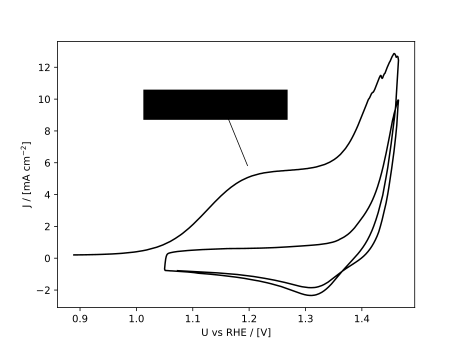
\includegraphics[width=0.5\textwidth]{04_Oxygen/fig/Ru_on_GO_naive.png}
	\caption{Initial cyclic voltammagrams of Ru on graphene oxide material from the lab in Fuzhou, in 0.5 M \ch{H2SO4}}
	\label{fig:Ru_on_GO_naive}
\end{figure}

During my external stay with professor Wen Zhenhai in Fuzhou, one of the first measurements we did with their newly built EC-MS setup (see Subsection \ref{subsec:setups}) was to determine the actual onset of OER from an acid electrocatalyst that they knew was unstable (the overpotential required to draw 10 mA started low but skyrocketed after a few minutes), but appeared highly active. This material, dispersed ruthenium on a high-surface-area graphene oxide, showed a strong oxidation wave starting before 1.4 V vs RHE with a large shoulder starting at 1.2 V vs RHE (Figure \ref{fig:Ru_on_GO_naive}). It was of interest whether all of the current in the wave at 1.4 V, or even 1.2 V if the catalyst was somehow ultra-activated in the beginning, could be attributed to \ch{O2} formation.

\begin{figure}[h]
	\centering
	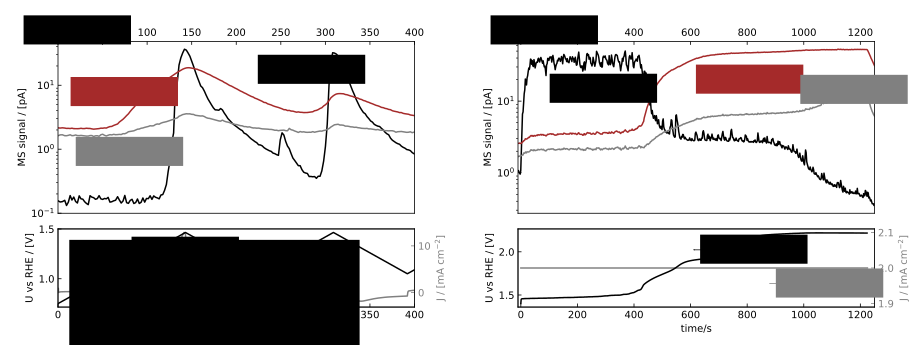
\includegraphics[width=1\textwidth]{04_Oxygen/fig/Ru_on_GO.png}
	\caption{EC-MS plots of Ru on graphene oxide material from the lab in Fuzhou, in 0.5 M \ch{H2SO4}. \textbf{(a)} initial cyclic voltammagrams and \textbf{(b)} constant-current experiment.}
	\label{fig:Ru_on_GO}
\end{figure}

Figure \ref{fig:Ru_on_GO}a shows the same cyclic voltammatry data with mass spectrometry detection of the products. Clearly, the ``ultra-low onset \ch{O2}'' above is not \ch{O2} but instead is revealed by the m/z=44 signal, implying \ch{CO2} evolution, to be oxidation of the graphene oxide support. This oxidation of the support continues into the main OER wave, and can also be seen in the second cycle. The onset for \ch{O2}, at about 1.33 V vs RHE, is remarkably low, indicating that the catalyst is highly active (though perhaps only as active as \ch{RuO2} films, see Section \ref{sec:low_O2}). However, there is less \ch{O2} in the second cycle, belying the catalyst's instability.

Figure \ref{fig:Ru_on_GO}b shows a 20-minute constant-current measurement in the EC-MS setup. At 2 mA/cm$^2$, it fails catastrophically at around 400 seconds into the experiment. At this point, the potential increases rapidly, and the 2 mA/cm$^2$ no longer goes to OER, but instead goes to oxidation of the substrate, as indicated by the switch from m/z=32 (\ch{O2}) to m/z=44 (\ch{CO2}) in the mass spectrometer. This is likely the point at which all of the ruthenium has dissolved or detached from the substrate. There is a m/z=28 signal which is attributed to cracking of \ch{CO2}, but, interestingly, at about 1100 s, the m/z=28 signal starts increasing independently of the m/z=44 signal. This is attributed to a new mechanism for oxidation of the carbon support at these high potentials ($>$2 V vs RHE) resulting in evolution of \ch{CO}. 

This illustrates the importance of product detection when measuring activity in the highly corrosive acid OER conditions.

\subsection{Nickel-iron: electrodeposited film vs annealed nanoparticles}\label{subsec:NiFe}

\begin{figure}[h]
	\centering
	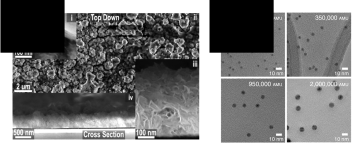
\includegraphics[width=1\textwidth]{04_Oxygen/fig/NiFe_foam_and_NPs.png}
	\caption{SEM images of NiFe-based OER catalysts \textbf{(a)}, Example of a high-loading, high-surface-area NiFe oxyhydroxide catalyst studied in the literature, taken from reference \citen{Batchellor2015}. \textbf{(b)}, Mass-selected vacuum-synthesized NiFe nanoparticles, from Paper \ref{Roy2018}.}
	\label{fig:NiFe_foam_and_NPs}
\end{figure}

As mentioned above, electrodes based on oxidized nickel and iron are used in industrial alkaline electrolyzer cells. However, the intrinsic OER activity of this electrocatalytic material is not well known, since it is typically used and studied in a highly porous foamy form\cite{Dionigi2016b}. An example, from ref \citen{Batchellor2015}, is shown in Figure \ref{fig:NiFe_foam_and_NPs}a. It is very difficult to estimate the intrinsic activity, i.e., the turn-over-frequency, of such materials because it is hard to determine how many active sites are accessible for the reaction. This was our primary motivation for studying a model system: vacuum-synthesized mass-selected \ch{Ni_{0.75}Fe_{0.25}} nanoparticles, characterized in detail in Paper \ref{Roy2018}.

The mass-selected nanoparticles were formed in a cluster source as follows\cite{VonIssendorff1999}: 
\begin{enumerate} 
	\item Atoms were freed from a solid metallic target (here \ch{Ni_{0.75}Fe_{0.25}}) by bombardment with a magnetically-bound plasma, i.e. magnetron sputtering. 
	
	\item These atoms were condensed into nanoparticles with a wide size distribution in an aggregation zone with a controlled temperature and argon pressure. Many of the nanoparticles are ionized, i.e. they carry a fundamental charge. 
	
	\item The charged nanoparticles are accelerated into a separation chamber and filtered according to m/z ratio using a modified time-of-flight mass spectrometer. 
	
	\item The beam of mass-selected nanoparticles is directed to a conductive substrate (here a 5mm Au stub) which is grounded via an ampmeter.  \label{item:deposition}
\end{enumerate}

The deposition current, measured in part \ref{item:deposition} above of the deposition technique, tells the number of nanoparticles deposited, since each deposited nanoparticle carries a fundamental charge. Since the size of the particles is known, this means that the mass loading is also known. Making an assumption about the shape of the nanoparticles, this means that the surface area is also known. In the case of the NiFe nanoparticles described here, SEM images (Figure \ref{fig:NiFe_foam_and_NPs}b) confirm a spherical shape. This is especially useful, because it means that, assuming the electrochemical reaction only occurs on the surface of the catalyst, that the number of available atomic sites can be calculated, and the turn-over frequency thus determined. These assumptions and results are discussed in more detail in Paper \ref{Roy2018} and in Section \ref{sec:lattice_O}.


\begin{figure}[h]
	\centering
	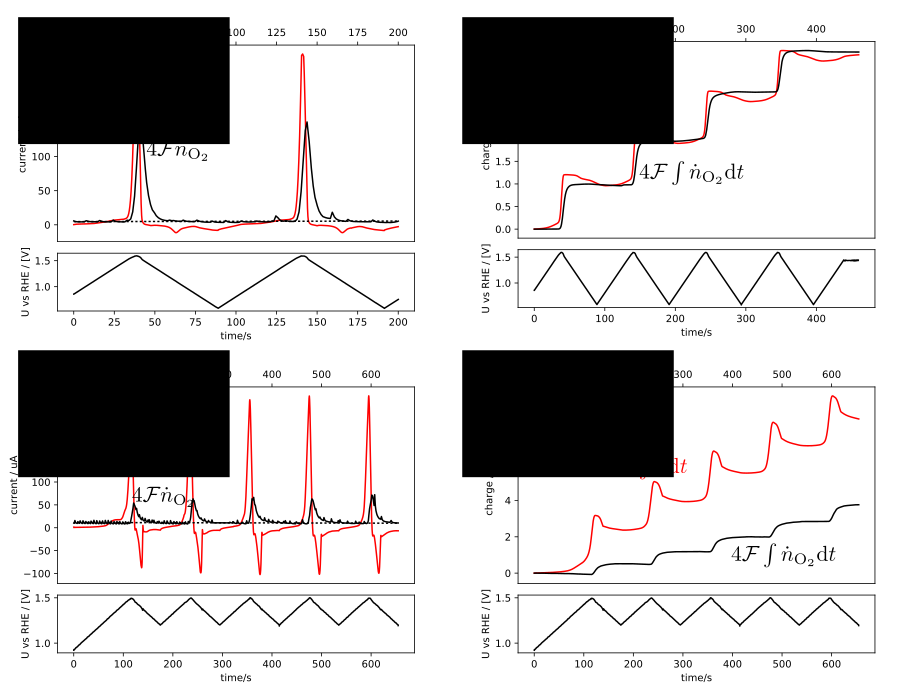
\includegraphics[width=1\textwidth]{04_Oxygen/fig/NiFe_current_vs_O2.png}
	\caption{Comparison of the electrode current and the OER current equivalent of the \ch{O2} signal in 0.1 M KOH for \textbf{(a-b)} 7 nm thermally annealed \ch{Ni_{0.75}Fe_{0.25}O_x} nanoparticles and \textbf{(c-d)} an electrodeposited \ch{Ni_{0.75}Fe_{0.25}O_xH_y} film. \textbf{(a)} and \textbf{(c)} show the (partial) current densities, while \textbf{(b)} and \textbf{(d)} show the integrals thereof.}
	\label{fig:NiFe_current_vs_O2}
\end{figure}

SEM and TEM images of the mass-selected nanoparticles also confirm that they are unchanged before and after reaction (Figures 2 and 4 of Paper \ref{Roy2018}). They OER activity is also stable over 1000 hours at 1.6 V vs RHE. These observations, taken together with the very small loading of the samples (approximately 150 ng of total Ni and Fe), indicate that charging or dissolution processes are negligible. We confirmed this using EC-MS by comparing the measured electrode current and the \ch{O2} signal during cyclic voltammatry in 0.1 M KOH of a sample with 150 ng of 7 nm mass-selected \ch{Ni_{0.75}Fe_{0.25}O_x} nanoparticles (the metal nanoparticles were annealed in \ch{O2} in the vacuum chamber for this sample). The results are shown in Figure \ref{fig:NiFe_current_vs_O2}a. The \ch{O2} signal, calibrated to mol/s as described in Chapter \ref{ch:tools}, is multiplied by four times Faraday's constant $\mathcal{F}$, which is the charge passed per mol of \ch{O2} formed by water oxidation, in order to plot on the same axis as the electrode current. The integrated current and the integrated OER partial current, shown in Figure \ref{fig:NiFe_current_vs_O2}b, match. This makes it clear that all of the net current can be accounted for by OER. The oscillating contribution of the \ch{Ni^{2+}/Ni^{3+}} cancels itself out when integrated.

For comparison, we synthesized a porous \ch{Ni_{0.75}Fe_{0.25}} oxy-hydrodixe film by electrodeposition, according to the method described in ref. \citen{Trotochaud2014a}, typical for the synthesis of \ch{NiFe}-based films studied in the literature\cite{Dionigi2016b}. In short, a current of - ​0.2 mA/cm$^2$ was passed through the substrate (a 5 mm Au stub) for 5 min in an electrolyte containing 100 mM \ch{Ni(NO3)2 * 6 H2O} and 5 mM \ch{FeCl2}. We then perform the same EC-MS experiment comparing the electrode current and evolved \ch{O2} during the first cyclic voltammagrams (Figure \ref{fig:NiFe_current_vs_O2}c and d). Unlike the case for the thermally oxidized nanoparticles, they do not match up over time. There is some net current transfer which cannot be accounted for by water oxidation. This may be attributed to charging of the film or dissolution of the metals, particularly Fe, which is known to leach. It could also be due to oxidation of adsorbed carbon-containing species (advantitious carbon), which would not be observed in EC-MS since the evolved \ch{CO2} would be captured by the alkaline electrolyte as \ch{CO3^{2-}}.

These results further highlight the need to measure \ch{O2} when determining the OER activity, especially for high-loading catalysts. Electrodeposited NiFe oxy-hydroxide films are known to be stable over longer periods of time, and are closely related to the catalyst used industrially in alkaline electrolyzer cells, but Figure \ref{fig:NiFe_current_vs_O2} makes it clear that, if \ch{O2} is not measured, one could easily overestimate the activity by just looking at the current passed during cyclic voltammatry.


\section{How low can we go?}\label{sec:low_O2}

Ruthenium dioxide can oxidize water at remarkably low overpotential in acidic electrolyte\cite{Miles1976, Reier2017}. However, it is not particularly stable, with anywhere from 0.01\% to 10\% of the current going to \ch{Ru} dissolution, depending on the preparation and experimental conditions\cite{Roy2018}. It is also used as a super-capacitor material\cite{Gonzalez2016} due to a very high pseudo-capacitance. This pseudocapacitance is due to the many redox transitions on the surface sites of \ch{RuO2} as well as the tendency of \ch{RuO2}, especially amorphous \ch{RuO2}, to form nano-scale interconnected domains, the surface of all of which are electrolytically accessible\cite{Yoshida2013}. In the previous Section, I illustrated that it is necessary to measure the \ch{O2} when studying OER catalysts. Together, the instability and high pseudo-capacitance (and thus large transient charging current) make this especially true for \ch{RuO2}-based electrodes. With this in mind, as well as the ability to do very sensitive isotope-labeling experiments, described in the next Section, we started a collaboration with Reshma Rao and professor Yang Shao-Horn at MIT to use our EC-MS system to study OER on \ch{RuO2}. One of the main goals was to see how low the onset potential for OER actually is.

\subsection{Sputtered \ch{RuO2} films}

\begin{figure}[h!]
	\centering
	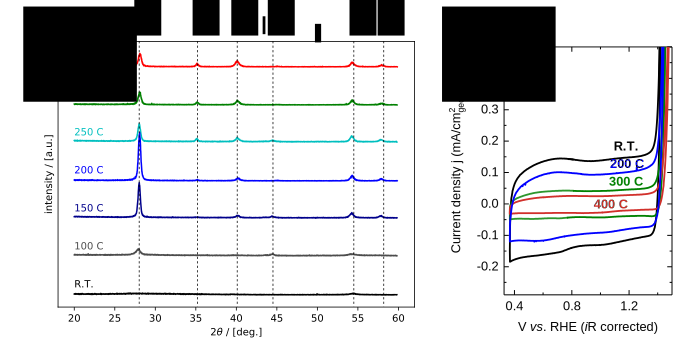
\includegraphics[width=0.8\textwidth]{04_Oxygen/fig/RuO2_film_char.png}
	\caption{Characterization of \ch{RuO2} films sputter-deposited at various temperatures. \textbf{(a)}, Grazing-incidence x-ray diffraction spectra. The theoretical peak positions of rutile \ch{RuO2} are indicated. \textbf{(b)} Cyclic voltammatry at a scan rate of 10 mV/s.}
	\label{fig:RuO2_char}
\end{figure}

To check whether and how activity, stability, and lattice oxygen involvement varied with crystallinity, we sputtered \ch{RuO2} at various temperatures. Reshma and I made the samples together when she visited DTU in September 2018. We sputtered \ch{RuO2} by reactive sputtering of a Ru sputter target with a magnetron sputter power of 300 W at a total pressure of 3 mTorr consisting of 80\% Ar and 20\% \ch{O2}. The films are characterized by grazing-incidence x-ray diffraction (GIXRD) and cyclic voltammatry in Figure \ref{fig:RuO2_char}.

\ch{RuO2} sputtered at room temperature (RT) appears amorphous, with no peaks visible in the diffractogram (Figure \ref{fig:RuO2_char}a). The films become more crystalline at higher sputtering temperature. However, while all the other peaks increase in intensity from RT to 400$^\circ$C sputtering, the (110) peak passes through a maximum at a sputtering temperature of 200$^\circ$C. This might indicate that a preferential orientation occurs at the right sputtering temperatures.

The relative surface areas of the samples, measured by electrochemical capacitance, however, decreases monotonically with higher sputtering temperature (Figure \ref{fig:RuO2_char}a). All of the films appear to be quite rough. Using a specific pseudo-capacitance (double-layer capacitance + redox charging) of 200 $\mu$F/cm$^2$, taken from Reference \cite{Yoshida2013}, the roughnesses factors go from $\approx$9 for the 400$^\circ$C-sputtered film to $\approx$60 for the RT-sputtered film. %Interesting, this roughness is on a 1-nm scale or smaller, as all films appear flat in AFM.

\begin{figure}[h!]
	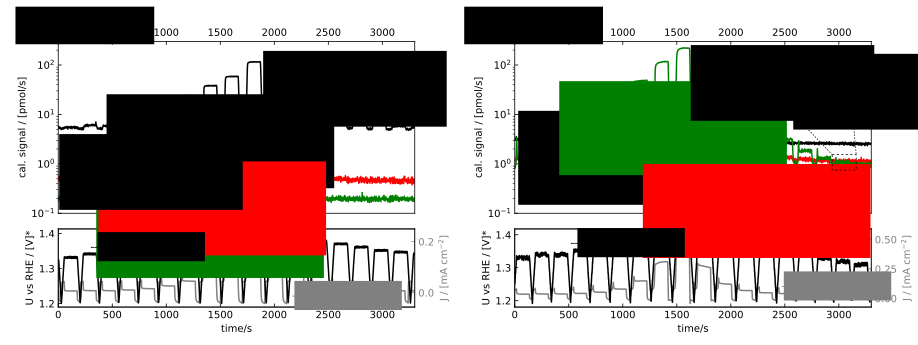
\includegraphics[width=1\textwidth]{04_Oxygen/fig/Reshma1_activities.png}
	\caption{Activity measurement of a \ch{RuO2} film sputtered at room temperature in 0.1 M \ch{HClO4} in \textbf{(a)} natural (99.8\% \ch{H2^{16}O}) water, and \textbf{(b)} 97\% \ch{H2^{18}O} labeled water.}
	\label{fig:Reshma1_activities}
\end{figure}


To measure the OER activities of the sputtered films in 0.1 M \ch{HClO4}, we scanned the potential at 5 mV/s from a ''resting potential'' of 1.2 V vs RHE to a working potential at which the OER measurement is made, holding each potential for 2 minutes. This was done to let the \ch{O2} signal reach a steady state at each potential and fall to the background level between activity measurements. The RHE potential of the reference electrode was always measured in the same electrolyte and the same setup using a platinum electrode and saturating the electrolyte in \ch{H2}, as described in Section \ref{sec:examples}. The \ch{O2} signal was calibrated by 5-minute constant-current OER steps (20 $\mu$A, 50 $\mu$A, and 100 $\mu$A) from a rutile \ch{IrO2} electrode measured in the setup on the same day, since \ch{IrO2} is known to be more stable than \ch{RuO2}\cite{Reier2017}.

The activity measurement for an R.T.-sputtered film is shown in Figure \ref{fig:Reshma1_activities}a. \ch{O2} production is stable during each 2-minute potential hold, giving a nice ''square-wave'' shape to the m/z=32 signal. The \ch{O2} production rate follows a neat Tafel relationship with applied potential, i.e. for a constant linear increase in potential step, the \ch{O2} signal increases by a constant factor. Specifically, the \ch{O2} production rate increases by about a factor of $\approx$2 for each 10 mV step in potential. More commonly, this is stated in the reciprocal form, as the extra potential required for a factor 10 increase in activity (a ''decade''), referred to as the Tafel slope. Here, the Tafel slope is $\approx$ 30 mV per decade

An oxygen signal is detectable down to 1.33 V vs RHE, a nominal overpotential of 100 mV. This was, to the best of our knowledge, already a record for detection of \ch{O2} from water oxidation. 

It should be emphasized that, while \ch{RuO2} is highly active, and the room-temperature-deposited film has the highest activity of the sputtered films, in line with its high roughness factor, we have no reason to believe that our \ch{RuO2} is more active than \ch{RuO2} reported in the literature. The detection of \ch{O2} at very low overpotential should, instead, be viewed as an accomplishment of the technique - specifically, the exceptionally high sensitivity of the chip-based EC-MS setup to gaseous products.

The detection limit of \ch{O2} is limited by the background of the m/z=32 signal, which is probably set by outgassing of the MS filament or other components in the vacuum chamber, or extremely small leaks. Since the background is thus dominated by natural \ch{O2}, which is 99.5\% \ch{^{16}O2}, the background at m/z=34 (\ch{^{16}O^{18}O}) and m/z=36 (\ch{O^{18}O2}) are considerably lower - by more than an order of magnitude comparing m/z=36 and m/z=32 as seen in \ref{fig:Reshma1_activities}a. Thus, additional sensitivity can be gained by isotopically labeling the oxygen in the electrolyte, and thus by extension, electrochemically-produced \ch{O2}.

Figure \ref{fig:Reshma1_activities}b shows an activity measurement of the same sample in 0.1 M \ch{HClO4} in 97\% \ch{H2^{18}O}. The y-axis in the top panel on the same log-scale as that in Figure \ref{fig:Reshma1_activities}a so that the activities and backgrounds are directly comparable Unfortunately, the m/z=36 background increases with the change of electrolyte, indicating that the \ch{O2} background in general comes partly from reaction of \ch{H2O} molecules, originating from the electrolyte, on the filament of the mass spectrometer. Due to this increase in background, the \ch{O2} detection limit is only improved by less than an order of magnitude. This, however, enables clear detection of \ch{O2} at 1.32 V vs RHE, a nominal overpotential of 90 mV.

\begin{figure}[h!]
	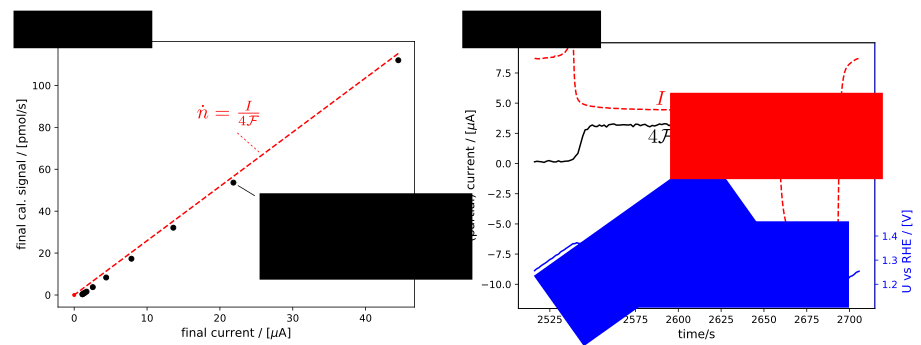
\includegraphics[width=1\textwidth]{04_Oxygen/fig/flux_and_current.png}
	\caption{Closer look at the activity measurement of a \ch{RuO2} film sputtered at room temperature in 0.1 M \ch{HClO4} in  natural (99.8\% \ch{H2^{16}O}) water. \textbf{(a)} Comparison of the averaged current and the \ch{O2} flux as measured during the final 30 seconds of each constant-potential step. The dotted line  \textbf{(b)} comparison of the instantaneous current (red) and \ch{O2} partial current density (black) during the activity measurement at 1.37 V vs RHE.}
	\label{fig:flux_and_current}
\end{figure}

As mentioned above, a concern with OER measurements in general, and in particular on \ch{RuO2}-based materials due to the high charging current and instability, is weather all of the electrode current is going to oxygen evolution. Figure \ref{fig:flux_and_current}a shows the value of the calibrated \ch{O2} signal vs the measured electrode current, averaged over the last 30 seconds of each 2-minute potential hold in Figure \ref{fig:Reshma1_activities}a. The theoretical line assuming 100\% Faradaic efficiency for \ch{O2} production is shown in red. The experimental data has the same slope as the theoretical line, but with a slight offset, with slightly less \ch{O2} than expected from the current. This is inconsistent with a significant dissolution current, as \ch{RuO2} dissolution increases with the current\cite{Cherevko2016}.

A more likely source of this offset is the charging current. Figure \ref{fig:flux_and_current}b shows a zoom-in of the potential step at 1.37 V vs RHE from Figure \ref{fig:Reshma1_activities}a. The calibrated \ch{O2} signal is multiplied by 4$\mathcal{F}$ to give a partial current density, and is plotted on the same axis (left y-axis) as the measured current. Here, we see that the measured current is dominated by capacitance while the potential is being scanned. This capacitive charging current continues during the potential hold, with the current only slowly approaching a steady state. The shape of the current during the constant-potential period is not completely exponential, but has a long tail, indicating that some parts of the electrode are harder to charge than others. In contrast, the \ch{O2} signal is stable during the potential hold. This comparison indicates that some of the current can still be contributed to the charging of the electrode even at the end of the two-minute potential hold.

\subsection{Hydrogen-bubble-template \ch{Ru} foam}

\begin{figure}[h!]
	\centering
	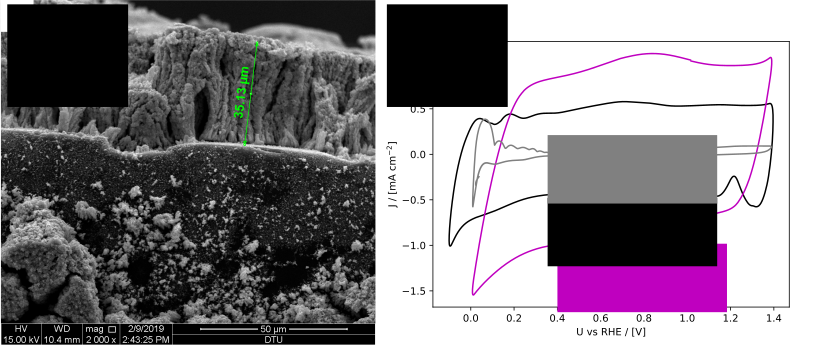
\includegraphics[width=0.9\textwidth]{04_Oxygen/fig/Ru_foam_characterization.png}
	\caption{\textbf{(a)} SEM image of Ru foam. \textbf{(b)} Cyclic voltammatry in 0.1 M \ch{HClO4} of a polycrystalline Pt electrode (gray), a room-temperature sputtered \ch{RuO2} film (black), and Ru foam (magenta). Note the different scan rates. The features just after the cathodic and anodic turns on the R.T. \ch{RuO2} cyclic voltammagram are artifacts of the electrode arrangement in the EC-MS setup.}
	\label{fig:Ru_foam_char}
\end{figure}

To see if we could push the limit of \ch{O2} detection to even lower overpotentials, we synthesized a high-surface-area ruthenium foam by the hydrogen-bubble template method. Choongman Moon and I made the first ones after useful input from Anna Winiwarter, who had optimized a procedure for depositing palladium foam (used for Paper \ref{Winiwarter2019}). Choongman made all of the subsequent films Briefly, a glassy carbon disk suspended by a copper wire fastened with a u-cup and Teflon table was immersed in a solution of 10 mM \ch{RuCl3} and 0.1 M \ch{HClO4}, opposite and parallel to a \ch{RuO2}/p+Si counter electrode held in place by gold wire. A bias of -6 V was applied to the working electrode with respect to the counter electrode for 10 minutes. Metallic Ru is deposited by reduction of the \ch{RuCl3} in solution. This results in an Ru ''foam'' layer that is extremely porous, as the Ru deposition is mass-transport limited and occurs simultaneously as rapid bubble formation by hydrogen evolution. Figure \ref{fig:Ru_foam_char}a shows a cross-sectional SEM image of the Ru foam.

Figure \ref{fig:Ru_foam_char}b shows cyclic voltammatry of the \ch{Ru} foam, with a \ch{RuO2} film sputtered at room temperature and a polycrystalline platinum stub included for comparison. Notice the different scan rates, necessary because the charging current of the Ru foam at 50 mV/s would max out the available bias between the working and counter electrodes. The electrochemically accessible surface area is clearly much higher than that of the room-temperature sputtered \ch{RuO2}, which already has a high roughness factor. Assuming the same specific capacitance of 200 $\mu$F/cm$^{2}$ from Reference \cite{Yoshida2013}, the roughness factor of the Ru foam is on the order of 2000.

\begin{figure}[h!]
	\centering
	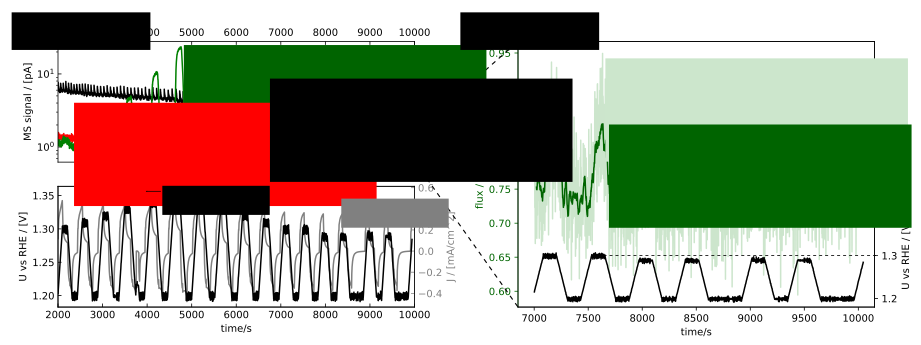
\includegraphics[width=1\textwidth]{04_Oxygen/fig/Ru_foam_activity.png}
	\caption{\textbf{(a)} EC-MS plot with raw MS data from an activity measurement at low overpotentials on the \ch{Ru} foam in 0.1 M \ch{HClO4} in 97\% \ch{H2^{18}O}. \textbf{(b)} Zoom-in on the lowest overpotentials, with the calibrated \ch{^{18}O2} (m/z=36) signal (faint green). The solid green trace is a 15-point moving-average smoothing of the \ch{^{18}O2} signal.}
	\label{fig:Ru_foam_activity}
\end{figure}

The results of an activity test on a Ru foam sample in labeled electrolyte are shown in Figure \ref{fig:Ru_foam_activity}a. \ch{^{18}O2} is detectable down to very low overpotentials. Note in the bottom panel that the charging current overwhelms the OER current, making the measurement of \ch{O2} absolutely necessary to determine the activity at low overpotentials. At the lowest potential measured, 1.29 V vs RHE, the signal can barely be discerned from the noise in the m/z=36 signal. This data point was repeated a total of four times with varying resting times in between in order to increase confidence that there is indeed a signal. The signal is more apparent when the data is smoothed with a 15-point moving average, which is shown as the solid green trace in Figure \ref{fig:Ru_foam_activity}b. Thus, we can claim to have detected \ch{O2} produced electrochemically at 1.29 V vs RHE, just 60 mV above the standard equilibrium potential.


\subsection{Turn-over-frequencies}\label{subsec:TOF}

\begin{figure}[h!]
	\centering
	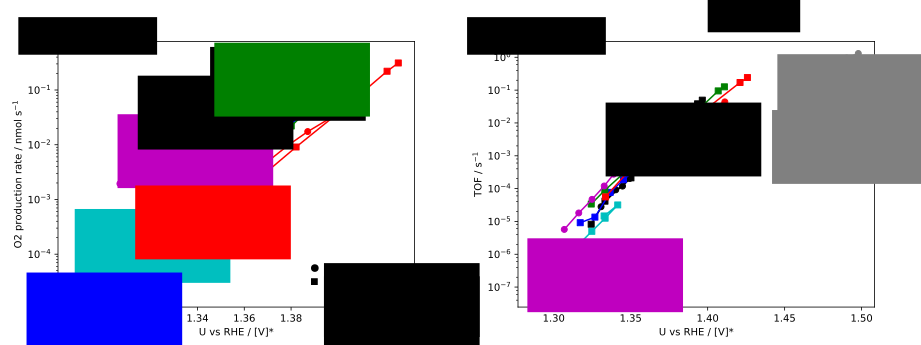
\includegraphics[width=1\textwidth]{04_Oxygen/fig/Ru_TOF.png}
	\caption{\textbf{(a)} \ch{O2} production rate as a function of potential for all measured sputtered \ch{RuO2} films and electrodeposited \ch{Ru} foams. \textbf{(b)} TOF for films and foams, assuming a specific capacitance of 200 $\mu$A/cm$^2$ and a an active site density of 2 per nm$^2$, correspondint to CUS sites on \ch{RuO2}(110)\cite{Rao2017}. [A] TOF for 3 nm \ch{RuO2} nanoparticles are from Paoli et al, Reference \citen{Paoli2015}.}
	\label{fig:Ru_TOF}
\end{figure}

Figure \ref{fig:Ru_TOF}a shows the \ch{O2} production rate, measured at m/z=32 or m/z=36 signal depending on the labeling of the electrolyte, averaged over the last 30 seconds of 2-minute potential holds for a number of \ch{RuO2} sputtered films and \ch{Ru} foams. All of the geometric areas were 0.196 cm$^2$. There is a large variation spanning approximately three orders of magnitude, with the \ch{Ru} foams producing \ch{O2} at a much higher rate at a given potential. This can, however, be explained fully by the higher surface area. In Figure \ref{fig:Ru_TOF}, the \ch{O2} production rate is normalized to the estimated number of active sites. This estimate was made using the following assumptions:

\begin{itemize}
	
	\item Assume a density of active sites equal to the density of CUS sites on the \ch{RuO2}(111) surface.
	
	\item Assume all surface contributing to the capacitance is active.
		
	\item Use the value 200 $µ$F/cm$^2$ determined by SAXS by Yoshida et al, Reference \citen{Yoshida2013}, applied to the portion of the CV's between 1.2 and 1.3 V vs RHE.
\end{itemize}

The first assumption seems reasonable, as (110) is the most stable surface of \ch{RuO2}, the CUS site is believed to be the active site\cite{Reier2017, Rao2017}, and metallic Ru will have an oxidized surface at the potentials of interest. The second assumption implies that there are no mass transport limitations in (\ch{H2O}) and out (\ch{H+} and \ch{O2}) of the porous structures of the amorphous \ch{RuO2}. This is reasonable at the low current densities achievable in the EC-MS setup, but might break down at higher current densities. The third assumption is based on a study using small-angle x-ray scattering (SAXS) to estimate the combined surface area of the condensed \ch{RuO2} aggregates in a series hydrous \ch{RuO2} electrodes\cite{Yoshida2013}. The authors of that study found that comparing the electrochemical charging current to the aggregate surface area thus estimated yielded a constant specific capacitance of 200 $\mu$F/cm$^2$, of which they estimate that $\approx$ 80 $\mu$F/cm$^2$ is double-layer capacitance and $\approx$ 120 $\mu$F/cm$^2$ is due to surface redox transitions. Here, I have implicitly assumed that all \ch{Ru} and \ch{RuO2} surfaces have the same double-layer and redox specific charging densities in the potential range 1.2 to 1.3 V vs RHE, chosen because all measurements include potential scans spanning this range.

Figure \ref{fig:Ru_TOF}b shows the turn-over-frequencies thus calculated. All of the \ch{RuO2} and \ch{Ru} samples converge on a common curve with $\approx$ 1 order of magnitude scatter. This adds validity to the assumptions made above, and suggest that the active sites are the same on the different materials. The curve has a slowly changing slope, with a Tafel slope of approximately 30 mV/decade at the upper end (1.38-1.42 V vs RHE), and a Tafel slope of approximately 20 mV/decade at the low overpotential range (1.30-1.34 V vs RHE). 

It is informative to compare these TOF values to TOF values measured and calculated by other means. In Reference \citen{Paoli2015}, Paoli et al report TOF values for mass-selected 3 nm \ch{RuO2} nanoparticles deposited with the same cluster source method used in Paper \ref{Roy2018}, also described briefly in Subsection \ref{subsec:NiFe}. Just like in that study, Paoli et al determine the number of active sites via the loading of the nanoparticles, which is known via the deposition current and the size of the nanoparicles. They compare two assumptions for the number of active sites: (1) that all Ru atoms are active sites (TOF$_{\text{bulk}}$), and (2) that only the Ru atoms at the surface of the \ch{RuO2} nanoparticles are active sites  (TOF$_{\text{surf}}$). These two TOF values are co-plotted with the present results in Figure \ref{fig:Ru_TOF}a. The TOF$_{\text{surf}}$ results for the nanoparticles continue the trend observed for the electrodeposited foams and sputtered films, with a further increase in Tafel slope at higher potentials, to about 60 mV/decade at 1.46 - 1.50 V vs RHE. This further supports the assertion that the active sites are similar however Ru or \ch{RuO2} are prepared, and that activity is limited to the surface, though this surface area can be quite large.

The changing Tafel slope has mechanistic implications\cite{Shinawaga2015}. Briefly, the oxygen evolution reaction consists of four steps, most simply written as\cite{Man2011, Busch2016}:

\begin{align}
\ch{H2O + $*$ -> $*$ OH + (H+ + e-)}\label{rxn:OER_s1}\\
\ch{$*$ OH -> $*$ O + (H+ + e-)}\label{rxn:OER_s2}\\
\ch{$*$ O + H2O -> $*$ OOH + (H+ + e-)}\label{rxn:OER_s3}\\
\ch{$*$ OOH -> $*$ + O2 + (H+ + e-)}\label{rxn:OER_s4}
\end{align}

In the limit that one of these steps, step $i$, is slower than the rest, then the rate is

\begin{equation}
r = k^0_i\theta_{i-1}\exp\left(\frac{\mathcal{F}}{RT}\alpha_i(U-U^\circ_i)\right)\,,\label{eq:rate}
\end{equation}
where $k^0_i$ is the rate constant for the $i$'th step, $U^\circ_i$ is its equilibrium potential. $\theta_{i-1}$ is the coverage of the reactant to that step, i.e., $\theta_0 = \theta_{*}$, $\theta_1 = \theta_{* \ch{OH}}$, $\theta_2 = \theta_{* \ch{O}}$, and $\theta_3 = \theta_{* \ch{OOH}}$. Finally, $\alpha_i$ is the symmetry factor to the reaction. The symmetry factor is the ratio of the change of the activation barrier of an elementary electrochemical reaction to the change in its overall $\Delta G$ resulting from a change in potential\cite{Bard2001}. Symmetry factors for elementary electrochemical steps are typically on the order of 0.5. Equation \ref{eq:rate} is thus an Arrhenius equation, with the activation barrier
\begin{equation}
E_{a,i} = \alpha_i\mathcal{F}(U - U^\circ_i)\,.
\end{equation}

%The potential dependence of the rate is thus
%\begin{equation}
%\frac{\partial r}{\partial U} =  k^0_i \left(\frac{\partial \theta_{i-1}}{\partial U} + \frac{F\alpha_i}{RT}\right)\exp\left(\frac{\mathcal{F}}{RT}\alpha_i(U-U^\circ_i)\right)\,,\label{eq:drate}\,
%\end{equation}

Taking the base-ten logarithm, 
\begin{equation}
\log(r) = \log(k^0_i) + \log(\theta_{i-1}) + \alpha_i\frac{\mathcal{F}}{RT\ln(10)}(U-U^\circ_i)\,,
\end{equation}
and differentiating with respect to potential,
\begin{equation}
\frac{\partial \log{r}}{\partial U} = \frac{\partial \log{\theta_{i-1}}}{\partial U} + \alpha_i\frac{\mathcal{F}}{RT\ln(10)}\,.
\end{equation}
This is the reciprocal of the Tafel slope. If the coverage of the reactant to step $i$ is constant ($\nicefrac{\partial \log{\theta_{i-1}}}{\partial U} = 0$), and the symmetry factor is 0.5, this gives 
\begin{equation}
\frac{\partial \log{r}}{\partial U} = \frac{1}{120\,\text{mV}}\,,
\end{equation}
or a Tafel slope of 120 mV per decade. 

The symmetry factor for an elementary step can not really be more than 1 (which would give a Tafel slope of 60 mV/decade with $\nicefrac{\partial \log{\theta_{i-1}}}{\partial U} = 0$), so the only way to have a Tafel slope of less than 60 mV per decade is to have a potential-dependent coverage of the reactant to the limiting step, i.e., 
\begin{equation}
\frac{\partial \log{\theta_{i-1}}}{\partial U} > 0\,.
\end{equation}
This implies that the $(i-1)$'th intermediate is not at saturation coverage, but is in equilibrium with empty sites ($*$) or other intermediates. The stronger the potential dependence (the greater $\nicefrac{\partial \log{\theta_{i-1}}}{\partial U}$, the smaller the Tafel slope. A Tafel slope of 20 mV/decade, observed for Ru Foam at the lowest potentials, implies (still assuming $\alpha_i=0.5$) that
\begin{equation}
\frac{\partial \log{\theta_{i-1}}}{\partial U} = \frac{1}{20\,\text{mV}} - \frac{1}{120\,\text{mV}} = \frac{1}{24\,\text{mV}}\,.
\end{equation}
or that the coverage of the $(i-1)$'th intermediate increases a factor 10 every 24 mV increase in potential.

In the assumption made above that one step is limiting, the potential-dependence of the coverage should be explained by the equilibrium between surface species, subject to the conservation law
\begin{equation}
 \theta_{*} + \theta_{* \ch{OH}} + \theta_{* \ch{O}} + \theta_{* \ch{OOH}} = 1
\end{equation}
The changing Tafel slope at low overpotential can thus provide crucial insight on which step is limiting and on the free energies of the intermediates. However, there are many free parameters, and the scatter of the data in Figure \ref{fig:Ru_TOF}b is large, making this challenging. Furthermore, the use of polycrystalline samples which may have more than one type of active site complicates the assumptions made above. This work is ongoing.


\subsection{The effect of \ch{O2} in the electrolyte}

Many fundamental studies of OER electrocatalysts involve electrochemical measurements in oxygen-saturated electrolyte. Indeed, the use of an overpotential referenced to 1.23 V vs RHE implies oxygen-saturated electrolyte, since the equilibrium potential is defined for all reactants and products at unit activity, namely 1 bar \ch{O2}. 

\begin{figure}[h!]
	\centering
	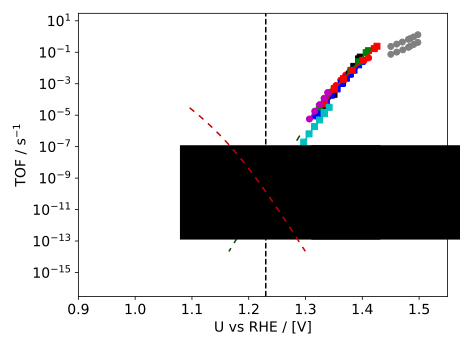
\includegraphics[width=0.5\textwidth]{04_Oxygen/fig/Ru_TOF_zoomout.png}
	\caption{Zoomed out TOF plot showing actual OER data from Ru and \ch{RuO2} (Figure \ref{fig:Ru_TOF}b), centered at the OER/ORR equilibrium potential at 1 bar \ch{O2}. A hypothetical ORR curve for a catalyst with ORR activity symmetrical to \ch{RuO2}'s OER activity is shown to illustrate that ORR is negligible at OER potentials.}
	\label{fig:Ru_TOF_zoomout}
\end{figure}

This is analogous to hydrogen evolution reaction (HER) studies, in which a hydrogen-saturated electrolyte is used. For the case of HER, which is reversible on the best catalysts such as platinum, the use of hydrogen-saturated electrolyte makes a crucial difference. Indeed, a significant hydrogen evolution current can be measured at 0 V vs RHE if the hydrogen is transported away from the electrode surface (Section \ref{sec:Hydrogen}). The importance of having the hydrogen-saturated electrolyte is that HER and the reverse reaction, the HOR, both occur at appreciable rates at the equilibrium potential.

However, at potentials sufficient to drive the highly irreversible OER, the equally irreversible oxygen reduction reaction (ORR) is negligible. This is abundantly clear when looking at Figure \ref{fig:Ru_TOF_zoomout}. Even if \ch{RuO2} was a symmetrical catalyst, i.e., as good at OER as ORR, the ORR current would still be approximately four orders of magnitude lower than the OER current at the  lowest potential at which we could detect \ch{O2} evolution, 1.29 V vs RHE. Furthermore, the scaling relations in oxygen evolution catalysts imply that a near-optimal OER catalyst like \ch{RuO2} is a rather bad ORR catalyst\cite{Busch2016}. 

\begin{figure}[h!]
	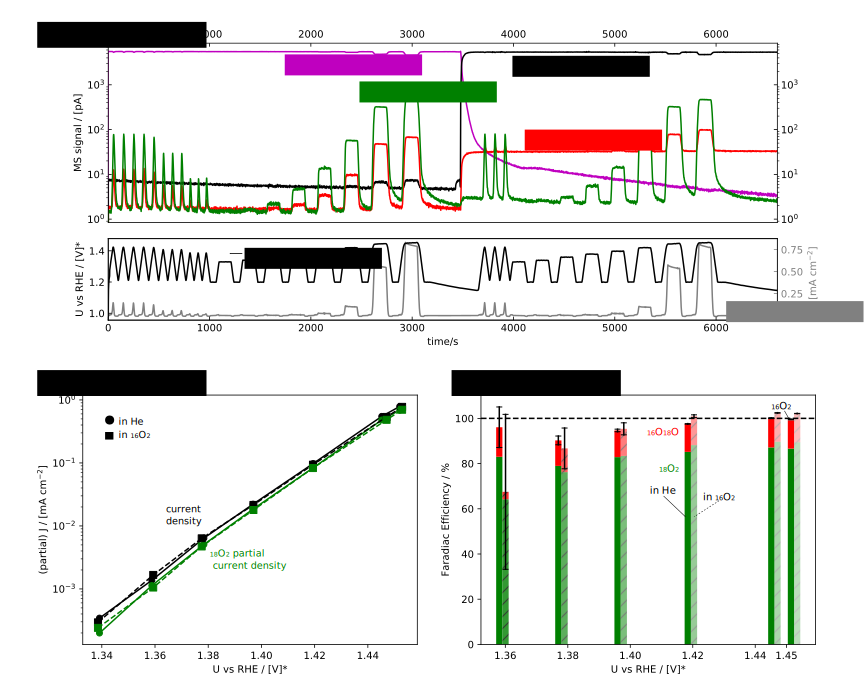
\includegraphics[width=1\textwidth]{04_Oxygen/fig/O2_vs_He_experiment_combined.png}
	\caption{\textbf{Activity of crystalline \ch{RuO2} in He-saturated and \ch{^{16}O2}-saturated 0.1 M \ch{HClO4} in \ch{H2^{18}O}.} \textbf{(a)} Experiment as an EC-MS plot. \textbf{(b)} The current density (black) and the partial current density for \ch{^{18}O} (green) at the end of each constant-potential step. \textbf{(c)} The Faridaic efficiencies for \ch{^{18}O2} (green) and \ch{^{16}O^{18}O} (red) as a function of potential. The error bar represents the uncertainty due to the standard deviation of the baseline m/z=34 MS signal.}
	\label{fig:He_vs_O2}
\end{figure}

Nonetheless, we decided to check if \ch{O2} saturation of the electrolyte had an effect. The use of isotope-labeled electrolyte enables the measurement by mass spectrometry of oxygen evolution under (un-labeled) \ch{O2}-saturated conditions. Figure \ref{fig:He_vs_O2}a shows such an experiment. The activity of a crystalline \ch{RuO2} electrode is first measured in labeled electrolyte saturated with inert gas. At approximately 3500 s, the electrolyte is quickly saturated with natural \ch{O2} through the membrane chip, and the activity experiment is repeated. The m/z=36 (\ch{^{18}O2}) signal looks identical in the two activity measurements, whereas the background of the m/z=34 (\ch{^{16}O^{18}O}) is shifted up by a background due to the natural isotopic distribution in the \ch{O2} carrier gas. 

The results are grouped by potential in Figure \ref{fig:He_vs_O2}b and c. There is no significant difference due to the presence of natural \ch{O2} in the current density or \ch{^{18}O2} partial current density (Figure \ref{fig:He_vs_O2}b). The increasing relative difference of the \ch{^{18}O2} partial current density and the total current density and the total current density at smaller overpotential can be attributed to residual electrode charging current during the last 30 seconds of each constant potential step from which the data are analyzed. There is no a significant difference in the Faradaic efficiency towards \ch{^{16}O^{18}O} (Figure \ref{fig:He_vs_O2}c), though the error bars in \ch{O2}-saturated electrolyte are much larger due to the m/z=34 background. Interestingly, the total labeled oxygen signal for the highest potentials, where the relative influence of background MS signal and electrode current loss to electrode are smallest, appears approximately 3\% larger in the \ch{O2}-saturated electrolyte. This is however believed to be due to an artifact whereby the small flux of \ch{O2} carrier gas into the vacuum chamber influences the overall sensitivity of the mass spectrometer. That approximately 12\% of the combined \ch{O2} signal is \ch{^{16}O^{18}O} reflects the composition of the electrolyte which is approximately 6\% \ch{^{16}O} after addition of \ch{HClO4}.

The fact that the presence of \ch{O2} has no influence on the overall OER current density of the catalyst should be expected, as the ORR current density is insignificant at potentials at which OER is significant. However, the same cannot be said for the individual steps of the reaction, for which the reverse elementary reaction might occur at a non-negligible rate. Thus, lack of a significant effect on the isotopic makeup of the evolved oxygen does have a mechanistic implication, if an unsurprising one: the limiting step in OER does not come before the formation of the O-O bond. If the limiting step were prior to the formation of the O-O bond (i.e., reactions \ref{rxn:OER_s3} and \ref{rxn:OER_s4} in equilibrium), then the O-O bond-forming step and all subsequent steps would be at equilibrium. There would then be a non-negligible rate for adsorption and dissociation of \ch{^{16}O2}, and recombination of the adsorbed \ch{^{16}O} with \ch{^{18}O} from the electrolyte, giving an increased \ch{^{16}O^{18}O} signal in the evolved oxygen. This does not appear to be the case at $U\ge1.42$ V vs RHE, though below this potential the uncertainty due to the m/z=34 background is too great to draw any conclusions. 





\section{To leave or to remain in the lattice}\label{sec:lattice_O}
%\section{What goes in can be pulled out}

In the previous section, I described the use of isotope-labeled electrolyte to take advantage of the low background signal for \ch{^{18}O2} and thus lower the overpotential at which electrochemically produced oxygen can be detected and quantified. In the final subsection, I used the lack of scrambling in \ch{^{16}O2}-saturated \ch{H2^{18}O} electrolyte to probe the rate-determining step of the OER an \ch{RuO2}. Both of these uses of isotope labeling in OER research are novel to the best of my knowledge. However, isotope labeling has been used extensively to probe another phenomenon: the involvement of lattice oxygen in the oxygen evolution reaction. 

\begin{figure}[h!]
	\centering
	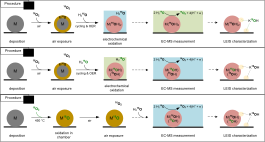
\includegraphics[width=1\textwidth]{04_Oxygen/fig/Strategies_diagram.png}
	\caption{Three strategies for isotope-labeling experiments intended to detect lattice oxygen involvement in the OER, diagrammed for the case of vacuum-synthesized \ch{NiFe} nanoparticles. Taken from Paper \ref{Roy2018}. \textbf{(a)} Strategy A involves mass spectrometric detection of evolved \ch{O2} (EC-MS step) for an unlabeled catalyst in labeled electrolyte. \textbf{(b)} Strategy B involves electrochemical labeling of an OER catalyst followed by EC-MS in an un-labeled electrolyte. \textbf{(b)} Strategy C involves direct preparation (here by annealing in \ch{^{18}O2}) of a labeled electrocatalyst followed by EC-MS in an un-labeled electrolyte.}
	\label{fig:strategies}
\end{figure}


\begin{table}
	
	\begin{tabular}{p{3cm}|p{3cm}|p{2cm}|p{2cm}|p{2cm}|p{2cm}|p{2cm}}
		Electrocatalyst & Preparation & Labeling & Electrolyte & Experiment & Result & Citation \\
		\hline
		Pt & On DEMS membrane, oxidized in 98\% \ch{H2^{18}O} & $\le$ 98\% \ch{^{18}O} & Natural 0.5 M \ch{H2SO4} or 1.0 M KOH & LSV, DEMS & no excess \ch{^{18}O} evolved & Willsau, 1985\cite{Willsau1985}\\
		\hline
		Ru and \ch{RuO2}& Sputtered onto Teflon DEMS membrane& Natural & 0.5 M \ch{H2SO4} in 90\% \ch{H2^{18}O} & CVs, DEMS & some excess \ch{^{16}O} evolved &  Wohlfahrt-Mehrens, 1987\cite{Wohlfahrt-Mehrens1987} \\ 
		\hline
		Hydrous \ch{IrO_x} & Thermal decomposition of \ch{HIrCl6} on Ti & Natural & 1 M \ch{HClO4} in 10\% \ch{H2^{18}O} & CVs, DEMS \& chip EC-MS & $>$ 1 ML excess \ch{^{16}O} evolved & Fierro, 2007\cite{Fierro2007}; rep. in Roy, 2018 \\
		\hline
		nanocrystalline \ch{RuO2} and \ch{Ru_{0.9}Ni_{0.1}O_{2-$\delta$}} & (co-)deposition on Ti mesh and annealing & Natural & 0.1 M \ch{HClO4} in 98\% \ch{H2^{18}O}& CVs, DEMS & Some excess \ch{^{18}O} evolved at high $\eta$ & Macounova, 2009\cite{Macounova2009}\\
		\hline
		Molecular Cobaltate Clusters &Electrodeposition of 0.5 mM \ch{Co^{2+}} in labeled phosphate & $\approx$ 87\% \ch{^{18}O} & Natural phosphate buffer& CP, integral headspace& 7-15\% of \ch{^{18}O} loading evolved& Surendranath, 2010\cite{Surendranath2010}\\
		\hline
		\ch{AuO_x} & Au oxidized at 2.0 V in 98\% \ch{H2^{18}O}& $\le$ 98\% \ch{^{18}O}& Natural 1 M \ch{HClO4}& LSV, OLEMS & $\approx$ 1 ML \ch{^{18}O2} evolved & Diaz-Morales, 2013\cite{Diaz-Morales2013} \\ 
		\hline
		polycrystalline, (110), (100), (101), and (111) \ch{RuO2} & oxidized in 98\% \ch{H2^{18}O} & $\le$ 98\% \ch{^{18}O} & Natural 0.1 M \ch{KOH} or 0.1 M \ch{H2SO4} & CVs, OLEMS & Little to no excess \ch{^{18}O} evolved & Stoerzinger, 2017\cite{Stoerzinger2017}\\
		\hline
		Spinel \ch{Co3O4} & as-received & Natural & 0.5 M KOH in 10\% \ch{H2^{18}O} & CVs, DEMS & 34\% ML excess \ch{^{16}O} evolved & Amin, 2017 \cite{Amin2017} \\
		\hline
		Spinel \ch{Co3O4} & electrochemically cycled in 10\% \ch{H2^{18}O} & $\le10\%$ \ch{^{18}O} & Natural 0.5 M KOH & CVs, DEMS & 12\% ML excess \ch{^{18}O} evolved & Amin, 2017 \cite{Amin2017} \\
		\hline
		\ch{LaCoO3} & solid-state synthesis, oxidized in 98\% \ch{H2^{18}O}  & $\le$ 98\% \ch{^{18}O} & Natural 0.1 M KOH & CVs, OLEMS & little to no excess \ch{^{18}O} evolved & Grimaud, 2017\cite{Grimaud2017}\\
		\hline
		\ch{La_{0.5}Sr_{0.5}CoO_{3-$\delta$}}& solid-state synthesis, oxidized in 98\% \ch{H2^{18}O}  & $\le$ 98\% \ch{^{18}O} & Natural 0.1 M KOH & CVs, OLEMS & Some excess \ch{^{18}O} evolved & Grimaud, 2017\cite{Grimaud2017}\\
		\hline
		\ch{Pr_{0.5}Ba_{0.5}CoO_{3-$\delta$}}& solid-state synthesis, oxidized in 98\% \ch{H2^{18}O}  & $\le$ 98\% \ch{^{18}O} & Natural 0.1 M KOH & CVs, OLEMS & Some excess \ch{^{18}O} evolved & Grimaud, 2017\cite{Grimaud2017}\\
		\hline
		\ch{SrCoO_{3-$\delta$}}	& solid-state synthesis, oxidized in 98\% \ch{H2^{18}O}  & $\le$ 98\% \ch{^{18}O} & Natural 0.1 M KOH & CVs, OLEMS & Some excess \ch{^{18}O} evolved & Grimaud, 2017\cite{Grimaud2017}\\
		\hline
		\ch{Ni_{0.75}Fe_{0.25}O_xH_y} film & electrodeposition & Natural & 0.1 M KOH in 97\% \ch{H2^{18}O} & CVs, chip EC-MS  & $\ll$0.1\% lattice O evolution & Roy, 2018\cite{Roy2018a} (Paper \ref{Roy2018})\\
		\hline
		\ch{Ni_{0.75}Fe_{0.25}O_xH_y}, 7 nm nanoparticles & cluster source, electrochem. oxidation & Natural & 0.1 M KOH in 97\% \ch{H2^{18}O} & CVs, chip EC-MS, ISS  & $\ll$0.1\% lattice O evolution & Roy, 2018\cite{Roy2018a} (Paper \ref{Roy2018})\\ 
		\hline
		\ch{Ni_{0.75}Fe_{0.25}O_xH_y}, 7 nm nanoparticles & cluster source, electrochem. oxidation in 97\% \ch{H2^{18}O} & Estimated 50\% \ch{H2^{18}O} & Natural 0.1 M KOH & CVs, chip EC-MS, ISS & $\ll$0.1\% lattice O evolution & Roy, 2018\cite{Roy2018a} (Paper \ref{Roy2018})\\ 
		\hline
		\ch{Ni_{0.75}Fe_{0.25}O_xH_y}, 7 nm nanoparticles & cluster source, thermal oxidation in \ch{^{18}O2} & Estimated 50\% \ch{H2^{18}O} & Natural 0.1 M KOH & CVs, chip EC-MS, ISS & $\ll$0.1\% lattice O evolution & Roy, 2018\cite{Roy2018a} (Paper \ref{Roy2018})\\ 	
		\hline
		Rutile \ch{IrO2} & Reactive sputter deposition with 99\% \ch{^{18}O2}& $\approx$ 99\% \ch{^{18}O} & Natural 0.1 M \ch{HClO4} & CP, OLEMS & little to no \ch{^{18}O} evolved& Geiger, 2018\cite{Geiger2018}\\
		\hline
		Hydrous \ch{IrO_x} & Potential cycling of sputtered \ch{Ir^{18}O2} film in 97\% \ch{H2^{18}O} & $\approx$ 97\% \ch{^{18}O}& Natural 0.1 M \ch{HClO4} & CP, OLEMS & some \ch{^{18}O} evolved& Geiger, 2018\cite{Geiger2018}\\
		\hline
	\end{tabular}
	\caption{Isotope-labeling experiments in the water oxidation electrocatalysis literature}\label{tab:lattice_lit}
\end{table}


Table \ref{tab:lattice_lit} shows a list of such experiments reported in the literature. The studies go all the way back to some of the earliest DEMS studies in the 1980's but have accelerated in the past couple years. The experimental methods (catalyst preparation, isotope labeling technique, electrolyte, and isotope exchange experiment measurement technique) are included to aid comparison of the various studies. One clear characteristic of this compilation is that there is no convergence yet in the literature on the best way to conduct these lattice exchange experiments.

The studies are approximately evenly split between DEMS or OLEMS for measuring the evolved oxygen isotopes. Most studies examine the oxygen evolved during potential sweeps (liniear sweep voltammatry, LSV) or cyclic voltammatry (CV), whereas only a few use constant-current measurements (CP). This is a problem because the redox changes during a potential sweep can destabilize electrode materials\cite{Kasian2016, Cherevko2016}, perhaps giving an isotope signal that would not be present in steady-state OER. Of those that measure a lattice oxygen evolution signal, some attempt to quantify the signal in terms of the total or surface oxygen loading of the catalyst\cite{Fierro2007, Surendranath2010, Diaz-Morales2013, Amin2017} whereas many observe an isotope signal but do not quantify it\cite{Wohlfahrt-Mehrens1987, Grimaud2017, Geiger2018}. 

The experiments differ mostly on how the catalyst and electrolyte are isotope labeled. Broadly, there are three strategies:


\begin{itemize}
	\item A. The catalyst is prepared without any labeled oxygen. The lattice oxygen is thus 0.2\% \ch{^{18}O}. Oxygen evolution is then measured in labeled electrolyte with an increased \ch{^{18}O} concentration\cite{Wohlfahrt-Mehrens1987, Fierro2007, Macounova2009, Amin2017, Roy2018a}.
	
	\item B. The catalyst is originally prepared with the natural isotopic ratio, but then it is used for oxygen evolution in a labeled electrolyte. If the OER mechanism involves an exchange between the lattice oxygen and the electrolyte, this will result in labeling of the electrocatalyst with a \ch{^{18}O} concentration in the active lattice sites up to that of the electrolyte. This electrochemically labeled catalyst is then transferred to un-labeled electrolyte, and the isotopic composition of the evolved oxygen is measured.\cite{Willsau1985, Diaz-Morales2013, Stoerzinger2017a, Amin2017, Grimaud2017, Roy2018a}.
	
	\item C. The final strategy is to prepare the catalyst from the start with labeled oxygen, and then measure the isotopic composition of the the \ch{O2} evolved in labeled oxygen. Techniques to synthesize a labeled catalyst include electrodeposition in labeled electrolyte\cite{Surendranath2010}, heating a metal precursor in a \ch{^{18}O2} atmosphere\cite{Roy2018a}, and reactive sputtering with \ch{^{18}O2} in the sputtering plasma\cite{Geiger2018}.
\end{itemize}

These three strategies are illustrated schematically for the case of mass-selected nanoparticles in Figure \ref{fig:strategies}, taken from Paper \ref{Roy2018}. The coming Subsection motivates and describes the isotope labeling studies in that paper.

\subsection{Determining the TOF in NiFe nanoparticles}

As described in Subsection \ref{subsec:NiFe}, our group prepared a model system of vacuum-synthesized, mass-selected \ch{Ni_{0.75}Fe_{0.25}} nanoparticles in order to determine the turn-over frequency (TOF) of nickel-iron based electrodes for water oxidation in alkaline media. The full story is in Paper \ref{Roy2018}. 

\begin{figure}[h!]
	\centering
	\includegraphics[width=1\textwidth]{04_Oxygen/fig/NiFe_redox_vs_surface.png}
	\caption{Activity and redox feature of \ch{NiFeO_xH_y} nanoparticles in 1.0 M KOH. \textbf{(a)}, Turn-over frequencies using three different assumptions about the number of active sites, as a function of particle size. \textbf{(b)}, Cyclic voltammagrams of all samples used for the TOF measurements, zoomed in on the redox feature. \textbf{(c)}, The number of electrons transfered in this redox feature, normalized to the calculated number of surface atoms, as a function of particle size. Taken from Paper \ref{Roy2018}. (a) is from the main text and (b) and (c) are from the SI.}
	\label{fig:redox_vs_surf}
\end{figure}

The activity of nanoparticles for a given (electro)catalytic reaction is influenced by the nanoparticle size\cite{Mistry2016b}. In general, the mass-normalized activity increases with smaller nanoparticle size, as the surface area to volume ratio of a particle increases with decreasing diameter. However, this is not always the case. If, for example, the reaction is most facile a specific type of surface site (for example, if terraces are more active than edges), then there can be an optimum in nanoparticle size. This appears to be the case, for example, in \ch{CO2} reduction to hydrocarbons on copper nanoparticles\cite{Reske2014} and oxygen reduction on platinum nanoparticles\cite{Hernandez-Fernandez2014}. Alternately, if the bulk of a material is active for a reaction, as has been suggested for NiFe-based OER catalysts\cite{Batchellor2015, Doyle2017}, then the mass-normalized activity would not vary with nanoparticle size.

As mentioned in Subsection \ref{subsec:NiFe}, the cluster source synthesis enables us to know the exact mass and surface loading of each sample. Figure \ref{fig:redox_vs_surf}a shows the turn-over frequency at 1.53 V as a function of nanoparticle size vs RHE calculated with three different assumptions about the number of active sites: TOF$_{\text{bulk}}$ assumes all metal atoms are active, TOF$_{\text{surface}}$ assumes metal atoms on the outer surface of the nanoparticle are active, and TOF$_{\text{redox}}$ assumes one active site per electron transfered during the \ch{Ni^{2+}/Ni^{3+/4+}} redox couple just before the onset of OER. This redox couple is shown for all of the samples in the CV's in Figure \ref{fig:redox_vs_surf}b.

Since TOF$_{\text{bulk}}$ (which is proportional to the mass-normalized activity) does indeed decrease with increasing nanoparticle size, we conclude that the bulk of these nanoparticles do not participate in the oxygen evolution reaction. On the other hand, the TOF$_{\text{surface}}$ and TOF$_{\text{redox}}$ do not show clear trends with nanoparticle size. This is consistent with each surface atom being an active site, or with each electron transferred during the redox wave representing an active site. For the electrodeposited NiFe LDH (also described in Subsection \ref{subsec:NiFe}), the exact loading was unknown and so only TOF$_{\text{redox}}$ is shown. This is lower than TOF$_{\text{redox}}$ for the nanoparticles, indicating either that the number of electrons transferred in the redox feature is not the best way to measure the number of active sites, or that the activity of the active sites differ for these two differently synthesized materials.

Figure \ref{fig:redox_vs_surf}c shows the number of redox electrons per Ni atom (black, left y-axis) and per surface Ni atom (red, right y-axis). The latter is equal to the ratio between TOF$_{\text{surface}}$ and TOF$_{\text{redox}}$. For the smallest nanoparticles, the entire nanoparticle appears to be redox active, with approximately one redox electron transferred per nickel atom in the sample, whereas for the larger nanoparticles, there are fewer than 1 electron transferred per nickel atom, indicating that the particles have a redox-inactive core. There are three to five electrons transferred per surface Ni atom, indicating that the redox feature penetrates below the outer surface of the nanoparticles. The question is then whether the redox-accessible portion of the nanoparticle is also OER active. This is illustrated in Figure \ref{fig:NP_diagram}.

\begin{figure}[h!]
	\centering
	\includegraphics[width=0.8\textwidth]{04_Oxygen/fig/NP_diagram.png}
	\caption{Two competing models of the nickel redox feature and oxygen evolution in NiFe nanoparticles. \textbf{Left}, The redox-active near-surface region is permeable to \ch{OH-} and \ch{O2}, and contributes to the OER. \textbf{Right}, The redox-active near-surface region is only accessible by proton shuttling and does not contribute to OER. The diagram on the far left of a proposed layered structure for the redox-permeable NiFeOOH region is from Friebel, 2015, which is Reference \cite{Friebel2015}.}
	\label{fig:NP_diagram}
\end{figure}

The question of whether the redox-active near-surface region contributes to OER is related to the question of which species carries the charge in and out of this region during the redox transition. If it is \ch{OH-}, then it is reasonable to believe that \ch{H2O} and \ch{O2} can also escape, and the near-surface region can contribute to the OER, which in alkaline electrolyte can be written

\begin{equation}
\ch{4 OH- -> O2 + 2 H2O + 4 e-}\,.\label{rxn:OER_alkaline}
\end{equation}

Unfortunately, the transport mechanism involved in the nickel redox feature is still not known\cite{Dionigi2016b}. It is often written by the nominal reaction 
\begin{equation}
\ch{Ni(OH)2 -> NiOOH + (H+ + e- )}\,,\label{rxn:Ni_redox}
\end{equation}
but in addition to protons, hydroxide and solvated cations have all been suggested as possible charge carriers\cite{WehrensDijksma2006}.

We therefore sought to answer the question by another means. We reasoned that, if the redox-active subsurface region participated in the oxygen evolution reaction, then the \ch{H2O} and/or \ch{OH-} originally in that region would be oxidized to \ch{O2} which we could differentiate from oxidation of the bulk electrolyte by isotope labeling. We performed the three isotope-labeling procedures described in Figure \ref{fig:strategies} on mass-selected 7nm NiFe nanoparticles:


\begin{figure}[h!]
	\centering
	\includegraphics[height=0.8\textheight]{04_Oxygen/fig/Roy2018_raw_results.png}
	\caption{EC-MS results for isotope experiments on \textbf{(a-c)} NiFe NP’s (a, b, and c correspond to procedures A, B, and C in Figure \ref{fig:strategies}); and \textbf{(d)} an electrodeposited NiFe thin film and \textbf{(e)} an \ch{IrOx} thin film produced by thermal decomposition of \ch{HIrCl6} in air, by procedure A. The signal for \ch{O2} produced in the largest portion by oxidation of the electrolyte (m/z=36 for procedure A and m/z=32 for procedures B and C) is plotted on the right y-axis, and the other \ch{O2} isotope(s) on the left y-axis. m/z=32 is omitted as a minority isotope since it is dominated by the background due to residual natural \ch{O2}. (f) The excess minority isotope (\ch{^{16}O} for procedure A and \ch{^{18}O} for procedures B and C) is quantified and normalized to (solid bars, left y-axis) the number of surface atoms in the catalyst or to (hashed bars, right y-axis) the total \ch{O2} evolved during the part of the experiment shown here. From the SI of Paper \ref{Roy2018}}
	\label{fig:Roy2018_raw_results}
\end{figure}

For procedure A, the as-synthesized nanoparticles were cycled between 0.5 V and 1.6 V vs RHE in un-labeled electrolyte, to form the hydrated redox-accessible near-surface region implied by Figure \ref{fig:redox_vs_surf}c. The sample was then transferred to the EC-MS setup, where the cell was filled with labeled electrolyte (0.1 M KOH in 97\% \ch{H2^{18}O}), and the potential was cycled up to where oxygen was evolved (1.55 V vs RHE). The advantage to procedure A is that there is no doubt about the initial isotopic composition of the oxygen in the catalyst, as the electrode has only been exposed to natural oxygen. The disadvantage is that the \ch{^{16}O} impurity in the labeled electrolyte limits the sensitivity. 

For procedure B, the as-synthesized nanoparticles were cycled between 0.5 and 1.6 V vs RHE in labeled electrolyte. A disadvantage here is that there is inevitably less than perfect control over the isotopic composition of the electrocatalyst, since it must pass through natural air. We expect, as a worst case, that the oxygen in the catalyst consists of 50\% \ch{^{18}O}, due to formation of \ch{M^{16}O}, with M=\ch{Ni_{0.75}Fe_{0.25}}, when exposed to air and subsequent formation of \ch{M(^{16}OH)(^{18}OH)} when cycled in labeled electrolyte. This is indicated in Figure \ref{fig:strategies}.

For procedure C, the as-synthesized nanoparticles were left in the vacuum chamber, where \ch{^{18}O2} was dosed and the sample was heated to 450$^\circ$C. The nanoparticles were thus already oxidized when taken out into air, and presumably retained a high degree of labeled isotopic purity and the nominal \ch{M^{18}O} formula. However, the sample was then put directly into the EC-MS setup with un-labeled electrolyte, where the nanoparticles likely hydrated to \ch{M(^{16}OH)(^{18}OH)} as illustrated. In hindsight, it would have been better to cycle the particles in labeled electrolyte prior to EC-MS testing to achieve a nominal \ch{M(^{18}OH)2} formula.

In addition to the NiFe nanoparticles, we also tested an electrodeposited NiFe oxyhydroxide film (described in subsection \ref{subsec:NiFe}) in the same electorlyte, and an \ch{IrOx} material produced by thermal decomposition of \ch{HIrCl6}. The latter material was produced by dropcasting a solution of 5 mM \ch{HIrCl6} on a titanium stub and annealing in air at 500$^\circ$C for two hours. This is the same material tested for lattice exchange in Fierro et al, 2007, which is Reference \ref{Fierro2007}. In that study, the authors saw a significant amount of lattice oxygen evolution as an excess \ch{^{16}O} signal during the first cyclic voltammagrams in \ch{^{18}O}-labeled electrolyte (see Table \ref{tab:lattice_lit}). Both the NiFe oxyhydroxide electrodeposited film and the thermal decomposition \ch{IrOx} samples were tested according to Procedure a: They were prepared with the natural isotope ratio, and tested for lattice exchange in labeled electrolyte. The NiFe film was tested in 0.1 M KOH in 97\% \ch{H2^{18}O} like the NiFe nanoparticles. The \ch{IrOx} was tested in 1.0 M \ch{HClO4} in 97\% \ch{H2^{18}O}. The higher concentration of \ch{HClO4} meant that the final isotopic purity of the electrolyte was lower.

The raw EC-MS results for these five isotope-labeling experiments (NP's procedure A-C, NiFe film and \ch{IrOx} procedure A) are shown in Figure \ref{fig:Roy2018_raw_results}a-e. 

Here, a quick note on this plotting form: in this type of isotope labeling experiments, a ''positive'' result is an isotope signal originating from the electrocatalyst, namely a (transient) isotopic composition of the evolved \ch{O2} that cannot be explained by the composition of the electrolyte. A ''negative'' result, on the other hand, is one in which the isotopic composition of the evolved \ch{O2} always reflects the isotopic composition of the electrolyte. It therefore makes sense to plot the results in a way where deviations of the measured \ch{O2} signal and the expected \ch{O2} from oxidation of the electrolyte are clearly visible. After trying a few different plotting strategies, our group thinks that the best way to do so, without hiding any information, is to co-plot the MS signals, scaled according to the expected ratio. This can be done by multiplying one of the signals by the expected ratio, or by using two y-axes scaled according to the expected ratio. The latter technique is used in Figure \ref{fig:Roy2018_raw_results}a-e. In each case, the ''expected ratio'' was taken to be the background-corrected steady-state ratio during a constant-current OER measurement taken right after these cycles.

When plotted this way, it is immediately clear that there is a very small amount of excess \ch{^{18}O} evolved in procedure B (Figure \ref{fig:Roy2018_raw_results}b) in the form of \ch{^{18}O2} (m/z=36) and \ch{^{18}O^{16}O} (m/z=34), a much larger amount of excess \ch{^{16}O} evolved from \ch{IrOx} (\ref{fig:Roy2018_raw_results}e) in the form of \ch{^{18}O^{16}O}, and little to no isotope signal in any of the other samples. 

The astute reader may have noticed a rather important experimental mistake: each experiment starts with an anodic scan from OCP, but for the NiFe nanoparticles in both procedures A (Figure \ref{fig:Roy2018_raw_results}a) and C (Figure \ref{fig:Roy2018_raw_results}c), the first cycle does is not anodic enough to produce a significant \ch{O2} signal, and the sample is cycled through the Ni redox couple before a significant amount of \ch{O2} is evolved. If oxygenated species are transferred or mobile during that redox reaction, then the labeled intercallated \ch{OH-} or \ch{O2} might escape to the bulk electrolyte before . We were aware of this mistake while preparing the manuscript, but did not get a chance to repeat these experiments, which were quite challenging for two reasons: (1) The cluster source synthesis was expensive and demanding, and (2) The membrane chips used in the EC-MS experiments at the time were not alkaline-resistant, and so chips would often breach during the measurement. So, after much frustration, we decided to use this data. We concluded, however, that it did not influence the interpretation of the results, for the following reasons: (1) We figured that at least some of the \ch{O} species, such as those bound to nickel in \ch{OH} groups, would stay put during the redox reaction, and (2) The results for procedures A and C were broadly consistent with the results for procedure B (Figure \ref{fig:Roy2018_raw_results}b) and for the electrodeposited film (Figure \ref{fig:Roy2018_raw_results}c). In hindsight, this mistake is part of the simpler and more general mistake of using potential scans rather than constant-potential or (even better) constant-current

Even if this experimental mistake weakens the conclusion that the redox-active near-surface region does not participate in the OER, it does not invalidate these experiments as evidence for the other conclusion of the isotope-labeling experiments: lattice oxygen is not exchanged during the oxygen-evolution reaction. This is based on an assumption that lattice oxygen is not exchanged during the (near-)surface redox reaction. This may even be used as a definition for lattice oxygen.




\subsection{A contradiction}

The attentive reader may have noticed a contradiction:

In Section \ref{sec:low_O2}, I noted that the acid-electrolyte OER activities of all \ch{RuO2} films and \ch{Ru} foams converged when normalized to the capacitance of the films, which I pointed out is consistent with an assumption that all of the surface area accessible to the electrolyte for active charging is also active for the oxygen evolution reaction. However, in Paper \ref{Roy2018}, we argue that only the outer surface of the nanoparticles is active for alkaline-electrolyte OER, even though the Ni redox feature penetrates $\approx$ 3-5 monolayers into the nanoparticles. We motivate this argument by isotope-labeling studies that always show \ch{O2} with the same isotopic composition as that of the electrolyte, reasoning that OER activity below the surface would either involve lattice oxygen evolution or oxidation of low-mobility intercalated water. We hypothesize that the redox activity below the surface is only due to proton shuttling.

This contradiction is especially troubling in consideration of the fact that unlabeled \ch{RuO2} films also do not give an isotope signal during OER in isotope-labeled electrolyte. I.e., sputtered \ch{RuO2} also gives a negative result to Strategy A in Figure \ref{fig:strategies}). Apparently, the water in the porous structure of high-surface-area \ch{Ru} and \ch{RuO2} has no trouble diffusing out of the pores before the onset of OER, unlike our assumption for NiFe oxyhydroxide.

One motivation for these differing lines of reasoning for the two materials is that the porosity is on a different scale: whereas the nanoscale domains and cavities in hydrous \ch{RuO2} are on the order of a few nanometers\cite{Yoshida2013}, the spacing between the layers in \ch{NiFe} layered double hydride are only 0.4 to 0.8 nanometers apart and perhaps interconnected by hydrogen bonds, depending on the phase\cite{Dionigi2016b}. Thus, there is more room for water and other species to diffuse in and out of amorphous \ch{RuO2}. Another is the TEM images of the NiFe nanoparticles (Paper \ref{Roy2018}, Figure 4) which indicate that they are non-porous both before and after the reaction (unfortunately, we do not have TEM images on the sputtered \ch{RuO2} films).

Nonetheless, the uncertainty evident in this contradiction, together with the imperfections mentioned above of the isotope experiments in Paper \ref{Roy2018}, mean that the conclusion of no OER activity in the redox-active near-surface region should be taken with a grain of salt. We think that these issues should motivate research into the charge transfer and mass transport processes during redox processes at the oxide-electrolyte interface for oxygen evolution catalysts. A better understanding of these transport processes is essential for determining the number of sites that participate in the oxygen evolution reaction, which in turn is essential for developing catalysts with improved intrinsic activity\cite{Kibsgaard2019}. 



\subsection{Labeled \ch{RuO2} and \ch{IrO2} films}

\subsection{Using CO to get out the lattice oxygen}


\section{Evolving vs dissolving}\label{sec:dissolving}

It is notable that all of the materials that do not show an isotope effect in Table \ref{tab:lattice_lit}, with the possible exception of Pt sputtered on a Teflon DEMS membrane\cite{Willsau1985}, are compact and crystalline films or nanoparticles\cite{Stoerzinger2017, Roy2018, Geiger2018}. In contrast, most of the materials for which studies have seen evidence of lattice oxygen evolution are hydrous, porous, or high-surface-area materials \cite{Wohlfahrt-Mehrens1987, Fierro2007, Surendranath2010, Amin2017, Grimaud2017, Geiger2018}. The authors of these studies all concluded that lattice oxygen is involved in the oxygen evolution mechanism. Equivalently, this implies that an oxygen vacancy is present at some point the electrocatalytic cycle, like in the Mars van Krevelen mechanism from thermal catalysis. However, the observation of an isotope effect does not in itself prove that lattice oxygen evolution is part of a catalytic mechanism. It could, for example, merely part of a parasitic degradation side-reaction. Likewise, many of the studies are not quantitative, and the relative importance of the Mars-van-Krevelin mechanism and other potential OER mechanisms that do not involve lattice oxygen is rarely addressed. 

Lattice oxygen evolution is only compared to dissolution in one of the studies: Geiger et al, 2018, ref. \cite{Geiger2018}. In that study, the authors found that hydrous \ch{Ir^{18}O_x} formed by potential cycling of a sputtered \ch{Ir^{18}O2} film in \ch{^{18}O}-labeled electrolyte, showed lattice oxygen evolution but also increased iridium dissolution compared to the as-sputtered \ch{Ir^{18}O2} film. The authors did not detect lattice oxygen evolution from the as-sputtered film. This comparison of lattice oxygen evolution to dissolution is highly valuable, but the authors did not absolutely quantify the lattice oxygen evolution for direct comparison to dissolution. Particularly, the question I became interested in was: 

\begin{question}
How does the number of lattice oxygen atoms evolved ($n_{\ch{O}}$) compare to the number of metal atoms dissolved ($n_{\ch{M}}$)?\label{q:O_vs_M}
?\end{question}

Only if $n_{\ch{O}}\gg  n_{\ch{M}}$, can it be concluded that there is a catalytic mechanism contributing to oxygen evolution which involves lattice oxygen exchange - though this mechanism may still be such a minor portion of the overall oxygen evolution activity as to be of no practical importance. On the other hand, if $n_{\ch{O}}\le  n_{\ch{M}}$, then lattice oxygen evolution might just be part of an unwanted dissolution reaction.

To answer this question, I performed lattice oxygen evolution experiments of the type described in the latter half of the previous Section (Subsections \ref{subsec:Ru_exchange} and \ref{subsec:extraction}), but also collected the electrolyte periodically during the experiment for quantification of metal dissolution with ICP-MS. The procedure for collecting electrolyte during the experiment without losing electrochemical control is described in Subsection \ref{subsec:other_tools}.

I performed these isotope-labeling ``exchange vs dissolution'' experiments on sputtered \ch{Ru^{18}O2} and \ch{Ir^{18}O2} films, electrochemically labeled \ch{Ru} and \ch{Ir} films, and Ru foam. The results are described in the following Subsections.

\subsection{Sputtered \ch{Ru^{18}O2} and \ch{Ir^{18}O2} films}


\begin{figure}[t]
	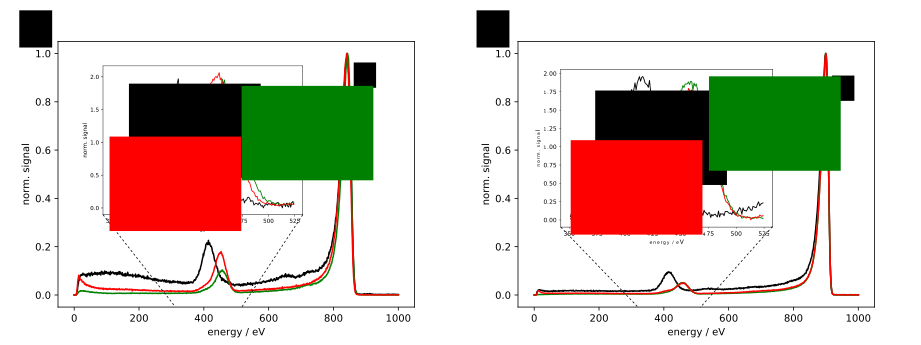
\includegraphics[width=1\textwidth]{04_Oxygen/fig/all_ISS_annotated.png}
	\caption{Ion-scattering spectrometry for isotope-labeled \textbf{(a)} \ch{RuO2} and \textbf{(b)} \ch{IrO2} sputtered films before (green) and after (red) 30 minutes of oxygen evolution at 0.5 mA cm$^{-2}$ in non-labeled electrolyte. Non-labeled films are included for reference (black). The spectra are normalized to the height of the metal peak. The insets show a zoom-in of the oxygen region and are normalized to the combined area of the oxygen peak(s).}
	\label{fig:ISS_O}
\end{figure}

Of the three strategies for oxygen labeling described in the begining of Section \ref{sec:lattice_O}, strategy C, whereby the as-synthesized catalyst is labeled with \ch{^{18}O}, is preferable whenever possible. It allows for a higher sensitivity than strategy A, in which an un-labeled catalyst is tested in labeled electrolyte, because the labeled electrolyte (typically $\le$ 97\% \ch{^{18}O}) is never as isotopically pure as un-labeled electrolyte (99.8 \% \ch{^{16}O}). On the other hand, it allows for a more well-defined electrocatalytic system than strategy B, in which an un-labeled as-synthesized electrocatalyst is treated electrochemically in labeled electrolyte before testing in un-labeled electrolyte, because the effectiveness of the electrochemical labeling procedure is rarely confirmed and may change the surface of the electrode.

We therefore prepared labeled \ch{Ru^{18}O2} and \ch{Ir^{18}O2} films by reactive sputtering of Ru or Ir with a sputtering plasma consisting of 80\% Ar and 20\% \ch{^{18}O2} (99\% isotopic purity). This produced an isotopically pure as-synthesized electrocatalyst for testing in un-labeled electrolyte.

Labeled oxide films of 25 nm nominal thickness (\ch{Ru^{18}O2}) or 10 nm thickness (\ch{Ir^{18}O2}) were prepared by sputter deposition on glassy carbon substrates with a 5 nm Ti sticking layer. The sputter deposition was done at room temperature, resulting in amorphous \ch{Ru^{18}O2}. The labeling of the as-deposited samples was confirmed by ion scattering spectroscopy as shown in Figure \ref{fig:ISS_O}. It is notable that the isotopic purity of the oxygen signal in ISS remained high even after the electrode was left out for several days in air, indicating that \ch{RuO2} and \ch{IrO2} do not exchange bound oxygen with the \ch{O2} or \ch{H2O} in air.

\begin{figure}[b!]
	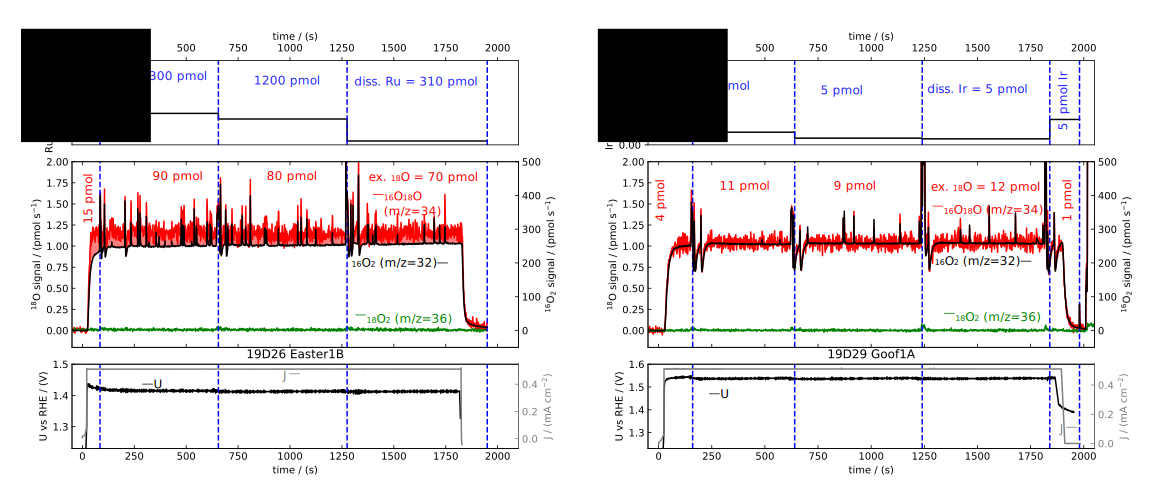
\includegraphics[width=1\textwidth]{04_Oxygen/fig/EC-MS-MS_plots.png}
	\caption{Metal dissolution (top panels) and lattice oxygen evolution (middle panels) from room-temperature sputter-deposited \textbf{(a)} \ch{Ru^{18}O2} and \textbf{(b)} \ch{Ir^{18}O2} films in un-labeled 0.1 M \ch{HClO4}. The \ch{O2} signals are measured \textit{in-situ} and plotted on two axes, scaled according to the natural isotopic ratio to show the excess \ch{^{16}O^{18}O}. The metal dissolution is was measured by determining by ICP-MS the concentration of metal in electrolyte samples taken at intervals indicated by the dotted blue lines.} 
	\label{fig:EC-MS-MS_plots}
\end{figure}

The labeled samples were placed in the chip-based EC-MS setup, oxygen evolution was run for half an hour at 0.5 mA/cm$^2$, and electrolyte samples were taken at intervals (approximately 2 min, 10 min, 20 min, and 30 min) for analysis by ICP-MS. The first ten minutes of electrolysis is shown in Figure \ref{fig:EC-MS-MS_plots}a for the labeled \ch{Ru^{18}O2} film, and in Figure \ref{fig:EC-MS-MS_plots}b for the labeled \ch{Ir^{18}O2} film. The results are plotted as EC-MS-MS plots, with the electrochemistry data in the lower panel, gas flux to the mass spectrometer in the middle panel, and averaged metal dissolution rate in the upper panel, all with a shared time axis. The gas MS data are plotted on two y-axes. The calibrated m/z=34 signal (\ch{^{16}O^{18}O}) is plotted on the right y-axis and the m/z=32 (\ch{^{16}O2}) signal plotted on the left y-axes. The two axes are scaled accordinig to the natural \ch{^{16}O^{18}O}/\ch{^{16}O2} ratio of 0.4\%. Thus, the two traces fall perfectly on top of each other when the oxygen evolved matches the natural isotopic ratio. For the case of \ch{Ru^{18}O2} there is a clear excess of \ch{^{16}O^{18}O} signal compared to the natural ratio. The excess is indicated in the plot with a light red highlight. In the first 10 minutes, there are approximately 100 pmol of lattice \ch{^{18}O} evolved. In comparison, approximately 150 nmol of oxygen was evolved in total. The mechanism by which lattice oxygen is evolved as \ch{O2} thus only accounts for $\approx$0.07\% of the total OER activity during the first ten minutes. For the \ch{Ir^{18}O2} film, the deviation of the \ch{^{16}O^{18}O} signal from the natural ratio is not immediately visible in Figure \ref{fig:EC-MS-MS_plots}, but integration indicates that there is a small excess of $\approx$ 15 pmol of \ch{^{16}O^{18}O} evolved during the first ten minutes, corresponding to less than 0.01\% of the total oxygen evolved. The rate of lattice oxygen evolution decreases only slightly during the remainder of the 30 minutes, such that 250 pmol of lattice oxygen is evolved during 30 minutes for \ch{Ru^{18}O2} and 35 pmol of lattice oxygen is evolved during 30 minutes for \ch{Ir^{18}O2}. In neither case was a significant \ch{^{18}O2} signal observed. 

It should be pointed out that, since the films studied here are isotope-labeled by reactive sputtering in vacuum with isotope-labeled oxygen, they have never been in contact with isotope-labeled water. Thus, incorporated \ch{H2^{18}O} can be ruled out as a source of the excess \ch{^{18}O} evolved, which is more difficult to exclude when films are electrochemically labeled. 

The vertical blue dashed lines indicate when electrolyte samples were taken. There is clear noise in the gas-phase MS data while electrolyte is flowing (middle panel), but with no loss of current control and potential measurement (bottom panel). The amount of metal in the electrolyte sample, in pmol, is indicated before each dotted blue line. This amount, divided by the length of time between electrolyte samples are taken, gives an average dissolution rate in pmol/s. For both the \ch{Ir^{18}O2} and \ch{Ru^{18}O2} samples, the highest dissolution rate was at the start of the electrolysis experiment, as the potential increased from OCP to the operating potential giving 0.5 mA/cm$^2$. In the case of \ch{Ru^{18}O2}, the average dissolution rate remained high, approximately 2 pmol/s, corresponding to a stability number on the order of 100. The amount of ruthenium dissolving into solution was approximately 10 times the amount of lattice \ch{^{18}O} evolved as \ch{^{16}O^{18}O}. For \ch{Ir^{18}O2}, on the other hand, the dissolution quickly lowers to a much smaller rate of ca 90 fmol/s, corresponding to a stability number of approximately 3x10$^4$. The amount of lattice oxygen evolved from \ch{Ir^{18}O2} actually exceeds the amount of iridium dissolved between all electrolyte samples excluding the ramp-up and ramp-down periods.

As a side note of potentially high interest: The apparent Ru dissolution rate for the last electrolyte sample (0.4 pmol/s) is much lower than for the previous two electrolyte samples (2 pmol/s). The main experimental difference is that the last electrolyte sample was taken after the applied potential was turned off, while the catalyst was at OCP. Electrolyte is flowing when the electrolyte sample is taken, and stagnant otherwise, so this may be a case of influencing the thing we are trying to measure. This result indicates that it may be the combination of applied potential and electrolyte flow that leads to \ch{RuO2} dissolution. More experiments are needed specifically probing the effect of electrolyte flow on ruthenium stability. If this is the case that ruthenium is many times more stable in still electrolyte than flowing electrolyte, it could have profound implications for PEM electrolyzers. Such a difference in stability could arise from a small concentration of dissolved ruthenium building up in the electrolyte when it is not flowing. This might imply that PEM electrolyzers with \ch{RuO2} designed to have a small anolyte volume with some concentration of dissolved ruthenium could stabilize ruthenium anodes. This would be important, as \ch{RuO2} requires less overpotential than the \ch{IrO2} catalyst currently used, and is (slightly) less scarce and thus more scalable. More experiments are needed.

Based on capacitance measurements, a monolayer of the labeled films corresponds to approximately 9 nmol of oxygen for \ch{RuO2} (roughness factor $\approx$ 50) and 3 nmol for \ch{IrO2} (roughness factor $\approx$ 25). The amount of lattice oxygen evolved in the full 30 minutes is thus $\approx$ 3\% of a monolayer for \ch{Ru^{18}O2} and $\approx$ 1\% of a monolayer for \ch{Ir^{18}O2}.

\begin{figure}[t]
	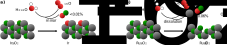
\includegraphics[width=1\textwidth]{04_Oxygen/fig/diagram_lattice_O_evolution.png}
	\caption{Lattice oxygen can either be due to (a) a Mars - van Krevelen type mechanism, as in the case of \ch{IrO2}, or (b) a dissolution side-reaction, as in the case of \ch{RuO2}.}
	\label{fig:exchange_diagram}
\end{figure}

If the lattice oxygen evolution is due to a Mars-van Krevelen type mechanism, then the oxygen isotope present in the electrolyte should be incorporated into the lattice, and should be present in the catalyst after the reaction. If, however, the lattice oxygen evolution is a side-product of a dissolution mechanism, then oxygen from the electrolyte would not be incorporated in the lattice. This is illustrated in Figure \ref{fig:exchange_diagram}. Ion-scattering spectrometry after OER can thus help distinguish between the possibilites. The red traces in Figure \ref{fig:ISS_O} indicate that little to no \ch{^{16}O} has been incorporated into the surface of the \ch{Ru^{18}O2} sample, whereas a small amount of \ch{^{16}O} has been incorporated into the surface of the \ch{Ir^{18}O2} electrode. This indicates that the very small amount of lattice oxygen exchange observed in \ch{IrO2} may in fact be due to a Mars - van Krevelen type mechanism, whereas the lattice oxygen evolution observed in \ch{RuO2} may just be part of a dissolution process. As an example of such a dissolution process, the \ch{^{16}O^{18}O} signal observed during OER for \ch{Ru^{18}O} could result from the decomposition in the chip or the vacuum chamber of \ch{RuO4} with at least one of the oxygen atoms from the lattice, as \ch{RuO4(g)} has been observed by mass spectrometry during OER on \ch{RuO2}.\cite{Geiger2018} 

These results from oxygen evolution on isotope-labeled films show that lattice oxygen evolution should not be interpreted as evidence of an important oxygen evolution reaction mechanism involving oxygen vacancies without careful, quantitative studies. Specifically, the activity of the lattice-involving mechanism should be compared quantitatively to the overall OER activity, and to the rate of metal dissolution. 

\subsection{Electrochemically labeled films}

We also performed the exchange vs dissolution experiments for \ch{Ru} and \ch{Ir} labeled electrochemically. Metallic films of 25 nm thickness (Ru) or 10 nm thickness (Ir) were prepared by sputter deposition on glassy carbon substrates with a 5 nm Ti sticking layer.

The metallic electrodes were placed in the EC-MS setup which was filled with labeled electrolyte (0.1 M \ch{HClO4} in 97\% \ch{H2^{18}O}), where they were first cycled between -0.05 V and +1.4 V (Ru) or +1.5 V (Ir) vs RHE, and then oxidized at +0.5 mA/cm$^2$ geometric current density for 10 minutes. They were then rinsed in natural water and put back in the setup with un-labeled electrolyte (0.1 M \ch{HClO4} in 99.8\% \ch{H2^{16}O}), and subject to a geometric current density of +0.5 mA/cm$^2$ for 30 minutes, with electrolyte taken at intervals for ICP-MS analysis. The results are shown in Figure \ref{fig:EC-MS-MS_EC}.

In both cases, an isotope signal can be seen in the start of the exchange experiment, but in both cases, the integrated excess \ch{^{16}O^{18}O} signal is less than one monolayer equivalent. It is larger for the oxidized \ch{Ru} (Figure \ref{fig:EC-MS-MS_EC}a) than for the oxidized \ch{Ir} (Figure \ref{fig:EC-MS-MS_EC}b). However, in contrast to the sputtered oxide films, in which the isotope signal was more or less steady throughout the 30 minutes of electrolysis, for these electrochemically oxidized films the excess \ch{^{16}O^{18}O} evolution is transient. This could indicate that labeled layer is quite thin and dissolves completely in less than 30 minutes. Indeed, the isotope \ch{^{16}O^{18}O} to \ch{^{16}O2} ratio has converged to the natural isotopic ratio for the oxidized \ch{Ru} film after approximately 9 nmol of \ch{Ru} has dissolved, corresponding roughly to one monolayer. This could indicate that only the outer monolayer had been labeled. Alternately, if the continued oxidation of the metallic film is faster than the dissolution, the labeled oxide layer could be burried beneath an un-labeled oxide layer. This is illustrated in the first panel of Figure \ref{fig:Pt_extraction_diagram}b. This is most likely the reason for the transience of the isotope signal for the iridium electrode, where significantly less than one monolayer of Ir has dissolved before the \ch{^{16}O^{18}O} to \ch{^{16}O2} ratio has converged to the natural isotopic ratio.

\begin{figure}[t]
	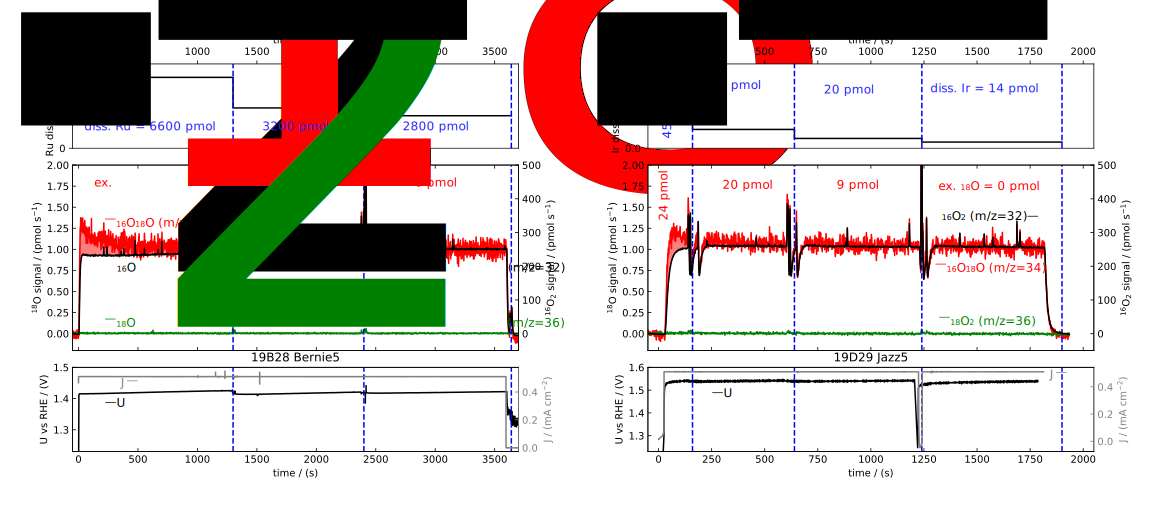
\includegraphics[width=1\textwidth]{04_Oxygen/fig/EC-MS-MS_plots_Electrochemically_labeled.png}
	\caption{Metal dissolution and lattice oxygen evolution from metallic \textbf{(a)} Ru and \textbf{(b)} Ir films in un-labeled 0.1 M \ch{HClO4} after formation electrochemical cycling and oxidation in \ch{^{18}O}-labeled electrolyte.
	}
	\label{fig:EC-MS-MS_EC}
\end{figure}
\begin{figure}[t]
	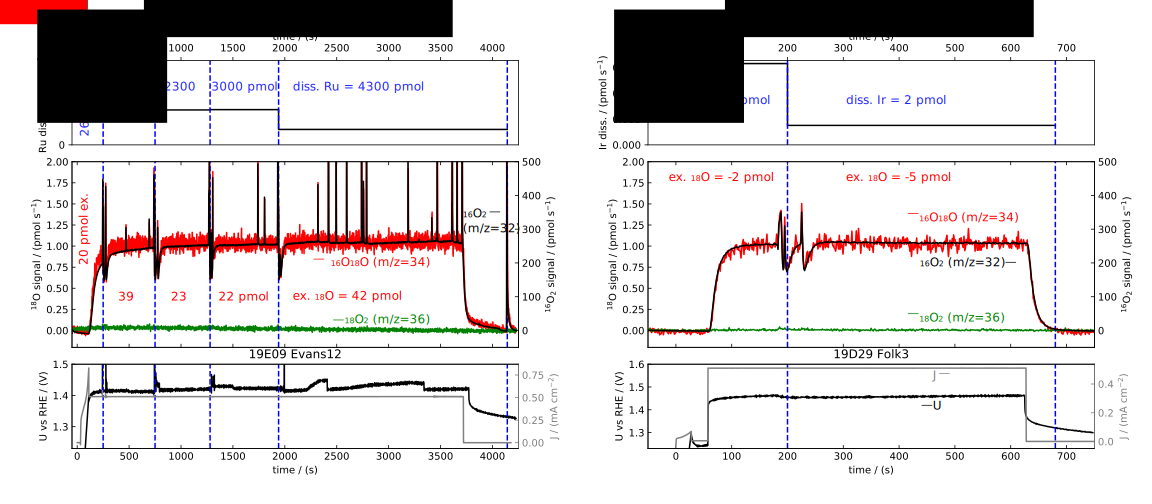
\includegraphics[width=1\textwidth]{04_Oxygen/fig/EC-MS-MS_plot_foam_and_control.png}
	\caption{Metal dissolution and lattice oxygen evolution in un-labeled 0.1 M \ch{HClO4} from \textbf{(a)} Ruthenium foam after oxidation in \ch{^{18}O}-labeled electrolyte, and \textbf{(b)} an un-labeled \ch{Ir^{16}O2} sputtered at 400$^\circ$C as a control.
	}
	\label{fig:EC-MS-MS_foam}
\end{figure}

In both cases, the amount of metal dissolution is much higher than it is for the sputtered oxide films. This is consistent with prior knowledge that \ch{RuO2} is more stable than \ch{Ru}\cite{Roy2018, Cherevko2016}, and \ch{IrO2} is more stable than \ch{Ir}\cite{Cherevko2016}. 

The same experiment was also performed for a \ch{Ru} foam electrode oxidized at 0.5 mA/cm$^2$ for 30 minutes. The result is shown in Figure \ref{fig:EC-MS-MS_foam}a. Again, the largest rate of excess \ch{^{18}O} evolution is at the beginning. The \ch{^{16}O^{18}O} to \ch{^{16}O2} ratio does not converge completely to the natural isotopic ratio during the 1 hr of measurement, but comes close during the final 30 minutes. This is despite the amount of dissolved ruthenium ($\approx$15 nmol) being much less than a monolayer-equivalent ($\approx$300 nmol) on this high-surface-area film. This film, like that tested in Figure \ref{fig:Evans_extraction} was only oxidized at constant current, and not cycled, in labeled electrolyte. Cycling the electrode in labeled electrolyte leads to a larger amount of labeled oxygen evolution in the exchange experiment (Figure \ref{fig:EC_Ru}). The near-convergence with less than a monolayer of \ch{Ru} dissolved may indicate that the labeled oxide layer becomes buried under an un-labeled oxide layer.

Finally, to validate that the excess \ch{^{18}O} in all of the previous experiments does indeed originate in the electrocatalyst (and not in the vacuum chamber, or an error in the data analysis), we performed a control experiment on an un-labeled \ch{IrO2} film. This film was sputtered on a Ti sticking layer on glassy carbon at 400$^\circ$C in isotopically natural \ch{O2}. The small negative values (-7 pmol total over 10 minutes of electrolysis) obtained when integrating the \ch{^{16}O^{18}O} signal and subtracting that expected based on the \ch{^{16}O2} signal should be taken as an indication of the uncertainty of the method.

\subsection{Exchange and extraction}

Finally, as the last result in this chapter, I show an exchange and extraction experiment (described in Subsection \ref{subsec:extraction}) done with electrolyte sampling for ICP-MS on a sputtered \ch{Ir^{18}O2} film. The entire experiment is shown in Figure \ref{fig:EC-MS-MS_extraction}. Because there's a lot going on, I show the electrochemical program both with the raw \textit{in-situ} MS data (Figure \ref{fig:EC-MS-MS_extraction}a), and again with analyzed \textit{in-situ} MS data and ICP-MS data (Figure \ref{fig:EC-MS-MS_extraction}b). 

\begin{figure}[b!]
	\includegraphics[width=1\textwidth]{04_Oxygen/fig/EC-MS-MS_IrO2_exchange_and_extraction.png}
	\caption{Sequential exchange (OER) and extraction (CO oxidation) experiments on a labeled \ch{Ir^{18}O} film in un-labeled 0.1 M \ch{HClO4}. \textbf{(a)}, raw EC-MS data with all masses plotted on a log scale. The highest mass signal is due to the He (m/z=4) or CO (m/z=28) carrier gas. An air signal is visible whenever electrolyte samples are taken for EC-MS as spikes in m/z=28 (\ch{N2}) and/or m/z=32 (\ch{^{16}O2}) though electrochemically produced \ch{^{16}O2} or \ch{CO} (m/z=28) sometimes interfere with these signals. \textbf{(b)}, Same data, analyzed, with ICP-MS data in the top panel. The labeled signals for \ch{^{16}O^{18}O} and \ch{C^{16}O^{18}O} are plotted on the left y-axis and the un-labeled \ch{^{16}O2} and \ch{C^{16}O2} signals are plotted on the right y-axis. The axes are scaled according to the natural \ch{^{16}O^{18}O} to \ch{^{16}O2} ratio, which is also the natural \ch{C^{16}O^{18}O} to \ch{C^{16}O2} ratio.
	}
	\label{fig:EC-MS-MS_extraction}
\end{figure}

From the left: starting just after t=0, an anodic geometric current density of +0.5 mA/cm$^2$ is applied for 23 minutes. Electrolyte samples are taken after 2 minutes, 10 minutes, and 20 minutes of electrolysis. Each time the electrolyte is exchanged to take a sample for ICP-MS, there is a spike in the m/z=28 signal due to \ch{N2} in the air-saturated electrolyte that is drawn into the cell. Unfortunately, the first electrolyte exchange appears to introduce a bubble, resulting in noise in the m/z=32 (\ch{^{16}O2}) and m/z=34 (\ch{^{16}O^{18}O}) signals starting then and continuing to the end of the electrolysis period. There is also some sporadic noise in the working-electrode potential, which may be because I bumped the alligator clip connecting to the working electrode while exchanging the electrolyte. However, the measured electrode current remains steady at the set value of +0.5 mA/cm$^2$.

Looking at the analyzed data for the same period, the results for lattice oxygen evolution and iridium dissolution are very much as in Figure \ref{fig:EC-MS-MS_plots}b: on the order of 30 pmol of both iridium dissolution and lattice oxygen evolution during the first 20 minutes of electrolysis, but with most of the iridium dissolution coming at the beginning while the potential is changed. Again, during steady electrolysis, the lattice oxygen evolution exceeds the iridium dissolution, indicating that there may be a minor OER mechanism involving lattice oxygen exchange. This confirms that the result is reproducible, and indicates that the method of subtracting the integrated \ch{^{16}O2} signal, weighted by the natural isotopic ratio, from the integrated \ch{^{18}O^{16}O} signal is robust even in the face of noisy data. Again, I emphasize that the lattice oxygen evolution is an extremely small portion - only 0.01\% - of the overall OER activity. 

Continuing towards the right in the raw data: after the electrolysis period, the potential is ramped down to a resting potential of 1.2 V vs RHE (with a small overshoot as I decided on what potential to rest at), and another electolyte sample is taken to see if this small potential ramp resulted in significant \ch{Ir} dissolution (it didn't). Then the carrier gas is changed from He (m/z=4) to CO (m/z=28) to begin the CO oxidation (extraction) portion of the experiment. A very small steady anodic current, on the order of 3 $\mu$A/cm$^2$, is detected right after introduction of \ch{CO}, together with a \ch{C^{16}O2} (m/z=44) signal, and is attributed to steady-state CO oxidation. This steady-state CO oxidation is continued for 15 minutes, during which two electrolyte samples are taken. The electrolyte sampling again brings air-saturated electroyte into the cell. This can no longer be seen in the m/z=28 signal, which is now dominated by CO, but can be seen as an \ch{^{16}O2} (m/z=32) signal. In the analyzed data, it appears that there is a small amount of excess excess \ch{C^{16}O^{18}O} in the \ch{CO2} evolved during this period, but the \ch{C^{16}O^{18}O} (m/z=46) background level is taken when the carrier gas is \ch{He}, and so I can't exclude the possibility that this is because of the effect of \ch{CO} on the background. The iridium dissolution during this period is not significantly above the ICP-MS detection limit of $\approx$ 1 pmol.

The CO oxidation activity at 1.2 V vs RHE is so low because, like \ch{PtO}, \ch{IrO2} is mostly inert for CO oxidation, whereas the metallic surface is active. At about 2500, the potential was scanned slowly (1 mV/s at first, then 5 mV/s) in the cathodic direction. Unlike Pt (Figure \ref{fig:Pt_extraction}), the cathodic scan did not result in a \ch{CO} oxidation transient. Apparently, there is not a sweet spot in between the potential at which an \ch{IrO2} surface is reduced and the potential at which \ch{$*$ OH} can no longer adsorb to oxidize CO by the Langmuir-Hinshelwood mechanism. In the absence of the desired transient, I allowed the cathodic scan to continue all the way down to 0 V vs RHE, where hydrogen evolution occurs, as evidenced by the cathodic current and the m/z=2 signal. This was a mistake, as it likely reduced much of the \ch{^{18}O} out of the surface layer of the electrode, and also dissolved some Ir, as dissolution is known to occur from metal oxide electrodes during the reductive potential sweep\cite{Cherevko2016}. The potential was then scanned anodic again at 5 mV/s, with CO oxidation starting in earnest at about 0.8 V vs RHE. A large transient in the current indicates that an adsorbed monolayer of \ch{CO} was stripped off (CO stripping). Then I went back and forth for a little bit before settling on 0.8 V vs RHE for steady-state extraction. The carrier gas is switched back to He at 3800 s, ending the CO oxidation experiment, and electrolyte is collected at about 4200s for ICP-MS. 

The scans between 2500 and 3200 were not ideal. In an optimal experiment, I would have only scanned the potential to slightly lower than 0.8 V vs RHE, perhaps 0.6 V vs RHE, and then back up, to reduce the surface enough that CO could adsorb, without reducing out lattice \ch{^{18}O}, and then go back up to 0.8 V vs RHE where the CO can be oxidized. Nonetheless, looking at the analyzed data, the procedure had the desired effect. A significant excess of \ch{C^{16}O^{18}O} is produced by CO oxidation, indicating that lattice oxygen can be involved in CO oxidation. 210 pmol of excess \ch{C^{16}O^{18}O} is evolved during CO oxidation, which is significantly more than the excess \ch{^{16}O^{18}O} during OER (40 pmol), and also significantly more than the Ir dissolved during this period (72 pmol) despite the accidental over-reduction of the sample. Because some of the \ch{C^{16}O^{18}O} is expected to lose the \ch{^{18}O} label due to homogeneous exchange with \ch{H2^{16}O} in the electrolyte, the actual amount of lattice O used to oxidize \ch{CO} was more than 210 pmol, though still less than a monolayer equivalent ($\approx$ 3 nmol).

Exchange and dissolution are measured for a second OER period after the CO oxidation experiment. When 0.5 mA/cm$^2$ is applied at 4500s and the potential ramps up to meet this current demand, a \ch{CO2} signal indicates that some \ch{CO} had remained adsorbed on the surface and was oxidized off by the increasing potential. There was a significant excess of \ch{C^{16}O^{18}O} in this \ch{CO2}, indicating that lattice oxygen was involved in stripping off the adsorbed \ch{CO}. There was also much more excess \ch{^{16}O^{18}O} in the \ch{O2} evolved during this second exchange experiment than the first, which may be due to a roughening or destabilizing effect of the potential cycling during the \ch{CO} oxidation portion of the experiment. 

It is worth pointing out that, despite these multiple independent clear observations of lattice oxygen reactivity, all of the lattice \ch{^{18}O}  evolved either in \ch{O2} or \ch{CO2} during the entire exchange + extraction + exchange experiment remained less than one monolayer equivalent.


\subsection{Conclusion and perspective on oxygen evolution experiments}

If, after reading this Chapter, you get an impression that all of the results remain a bit preliminary, please know that I am right there with you. 

The results presented in this Section, combining isotopic labeling by reactive sputtering with \ch{^{18}O2}, surface isotopic characterization by ISS, fluent electrolyte sampling during the experiments for dissolution measurements by ISS, and routine and confident detection of sub-picomol per second rates of lattice oxygen evolution, all came together during the last months of my PhD. The results presented in the previous Sections and Chapters (as well as Paper \ref{Roy2018}) have indicated some of the trial-and-error, mistakes, and development that was necessary to get there.

The goal is of course to use these tools and techniques to make breakthrough discoveries in OER catalysis that can lead to more efficient and cost-effective PEM electrolyzers. I expect that this could happen by the following paths:

\begin{itemize}
\item Insights based on the newly-detected changes in the Tafel slope of \ch{RuO2} (Section \ref{sec:low_O2}) will help inform theorists about which elementary steps and intermediates are most important in predicting materials that can catalyze the OER at high rates at lower overpotentials.

\item Quantitative comparison of lattice oxygen evolution, total oxygen evolution, and metal dissolution on an atom basis will help make it clear whether ''activating lattice oxygen'' is actually a desired strategy. Based on the results presented here so far on \ch{RuO2} and \ch{IrO2}, it seems that lattice-involving mechanisms are associated with instability and, in any case, only contribute a very small portion of the overall OER activity. Hopefully this will help direct the efforts of the research community.

\item The ease and sensitivity of quantitative OER activity measurements and metal dissolution measurements using the EC-MS setup and ICP-MS of the collected electrolytes will make these techniques a powerful screening tool for acid OER catalysts that are stable and active with less precious metal.
\end{itemize}

Next steps could include applying the techniques presented here to compare activity, exchange, and dissolution on calcined \ch{Ir} and \ch{Ru} containing catalysts more closely resembling the industrially-used ``dimensionally stabilized anodes''\cite{Escudero-Escribano2018}, and promising recently-reported materials based on alloying of Ir and Ru with non-noble metals\cite{Reier2015a, Seitz2016, Diaz-Morales2016a}. Some of this work is already being done by Mayrhofer and coworkers \cite{Geiger2018}, but the sensitivity of our EC-MS setup and the combination with ISS can add a lot. An obvious starting point would be to re-visit the thermal-decomposition \ch{IrO_x} result reproduced in Figure \ref{fig:Roy2018_raw_results} from Reference \citen{Fierro2007}, which showed significant lattice oxygen evolution but for which dissolution and ISS were not measured. 

In the next Chapter, the last Chapter of this Thesis, I will attempt to gauge the possible net impact of this work on the climate crisis described in Chapter \ref{ch:Intro}. To do so, I will assume that one or more of the possible impact paths above lead to a reduction of 0.1 mV in the overpotential needed to drive PEM electrolyzer cells, holding all else constant.
\clearpage

%

\chapter{The Net Carbon Impact of this PhD}\label{ch:impact}

\section{Assuming we do the right thing and tax carbon}
\section{How much difference a millivolt makes}\clearpage
	

\addcontentsline{toc}{chapter}{Bibliography} % sætter
\bibliographystyle{unsrt} 
\bibliography{PhD_thesis.bib}

%
%\begin{appendices}
\appendix
	
	\addtocontents{toc}{\protect\setcounter{tocdepth}{1}}
	
\chapter{Setup and technique details and instructions}\label{app:instructions}


The following procedures assume that the setup, hardware configuration, and Software interfaces have not changed since the publishing of this Thesis.

\section{Sniffer setup at DTU}\label{app:sniffer}


\begin{figure}[h!]
	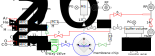
\includegraphics[width=\textwidth]{02_Tools/fig/setup_sniffer.png}
	\caption{Valve diagram of EC-MS setup at DTU. Adapted from Paper \ref{Trimarco2018}. Red: components installed since that publication. Green: The 6-way valve was removed since then as well as the pneumatic valves before the pressure controllers, which were re-purposed. Blue: The interface block, as well as the valve right before it, were replaced to minimize the intervening volume, enabling faster exchange of gases.}
	\label{fig:sniffer}
\end{figure}
Figure \ref{fig:sniffer} shows a valve diagram of the sniffer setup. Most of this setup was built during Daniel Trimarco's PhD project\cite{Trimarco2017_PhD}, and described in Paper \ref{Trimarco2018}. Colors indicate the parts that I have removed (green) or added (red) since Paper \ref{Trimarco2018}'s publication.

On the left of the diagram are mass flow controllers (MFC's) which can be used to switch between up to four gases at time. Switching between gases sharing an MFC, f.eks. Ar and He, requires pumping down behind the MFC through a line not shown. Moving right, we refer to the volume between Valves 7, 8, 9, 10, 11, and 12 and PC 1 as the \textit{gas manifold}. The gas manifold can be evacuated through Valve 7 and filled up from one of the MFC's while regulating the pressure with a pressure controller (PC), PC1.

Carrier gas from the gas manifold enters the interface block via Valve 8. The interface block guides it through the carrier gas reservoir channel of the chip, from which it fills the chip's sampling volume and saturates the electrochemical environment. Fast carrier gas exchange thus requires that the volume between valve 8 and the chip, the \textit{carrier gas inlet volume} is as small as possible. This is because the carrier gas inlet volume, unlike the gas manifold, cannot be pumped down, as the resulting vacuum in the sampling volume of the chip would suck in electrolyte. The design of the carrier gas inlet volume can also be optimized with regards to flow patterns to minimize mixing of the old and new carrier gas. 

We refer to the volume between PC1, PC2, and Valves 1, 5, 6, and 7 as the \textit{pumping manifold}. There are actually three possible ways to pump on the pumping manifold: (1) Directly to the \textit{roughing pump} (RP) through Valve 6, or (2-3) through a buffer volume and then a \textit{turbo molecular pump} (TMP or just turbo pump) via either a (2) valve 2 and a needle valve or (3) a gate valve. 
%Of these options, the direct roughing pump connection is the only one that can quickly remove a large amount of gas, as this would damage the turbo pump. Valve 14 should be closed while gas is fed directly to the roughing pump, as the pressure behind the turbo pump must also be kept low during operation. On the other hand, the turbo pump is required to reach high vacuum, which it can do slowly for a moderate amount of gas through the needle valve or quickly for a small amount of gas through the gate valve.

During operation, carrier gas is flowing from the gas manifold to the pumping manifold through the chip, and its pressure is regulated by PC2, which is set to 1 bar for all of the experiments in this Thesis. Excess carrier gas flows through PC2 to the pumping manifold where it is ultimately removed through the roughing pump, typically via the buffer volume and needle valve, so that valve 14 can remain open.

When a new chip is installed, the \textit{post-capillary volume} bound by the chip, Valve 13, and Valve 5 is vented to atmospheric pressure, and must be pumped down to high vacuum before connecting the experiment to the mass spectrometer. The mass spectrometer is always held at high vacuum by its own designated turbo and roughing pumps. The mass spectrometer of the sniffer setup is a Pfeiffer QMA125.

The procedures for chip pump-down and carrier gas exchange are described below.

An unusual feature of the sniffer setup, as mentioned in that Section, is that there are three ways to pump on the pumping manifold. Of these options, the direct roughing pump connection is the only one that can quickly remove a large amount of gas, as this would damage the turbo pump. Valve 14 should be closed while gas is fed directly to the roughing pump, as the pressure behind the turbo pump must also be kept low during operation. On the other hand, the turbo pump is required to reach high vacuum, which it can do slowly for a moderate amount of gas through the needle valve or quickly for a small amount of gas through the gate valve.

\subsection{Changing chip}
The procedure on this setup to change a chip is as follows:
\begin{enumerate}
	\item Isolate the chip: Make sure that Valves 13, 5, and 8 are closed, that no carrier gas is flowing, and that PC2 is closed (set to 2 bar). Double-check that Valve 13 is closed!!!
	
	\item Remove the old chip and put on the new chip.
	
	\item Close valves 1 and 14 and open valve 6 to connect the pumping manifold to the roughing pump. (The gate valve should be closed.)
	
	\item Open valve 5. This very quickly removes the majority of the gas from the post-capillary volume
	
	\item Close valve 6 and open Valve 1. Open valve 14.  
	
	\item Check the pressure displayed on the pressure guage (PG) of the buffer volume. The pressure in the buffer volume should already be less than 1 mbar. If not, the chip has not been installed correctly. If so, close valves 1 and 5 and start over.
	
	\item If the pressure in the buffer volume is greater than 0.3 mbar, start pumping through the needle by opening Valve 2.
	
	\item When the pressure in the buffer volume is less than 0.3 mbar (as will usually be the case right away after first roughing on the pumping manifold), open the gate valve. This is done by first deactivating 4 and then activating 3.
	
	\item When the pressure in the buffer volume is less than 0.0001 mbar, we can open to the mass spectrometer. Make sure that Valves 1 and 5 are open (so that the pressure on the buffer volume is equal to the pressure in the post-capillary volume), and open Valve 13.
	
	\item Immediately close Valve 5. This avoids making any subsequent mistake in which carrier gas enters the mas spectrometer via the pumping manifold. Also, close the gate valve. This is done by first deactivating 3 and then activating 4.
\end{enumerate}


\subsection{Changing carrier gas}
The procedure on this setup to change carrier gases is as follows. We will use the example of changing from He to \ch{H2}. This is what is done in Figure \ref{fig:RHE_cal}.

\begin{enumerate}
	\item At first, He is flowing through MFC1 at 1 ml/min and continues through Valve 9, Valve 8, the chip, PC2 (set to 1 bar), Valves 1 and 2, the turbo pump, Valve 14, and the roughing pump.
	
	\item Close valve 8. There is a reservoir of He in the interface block which will continue to fill the sampling volume of the chip for some time. Thus, the electrochemistry experiment can continue and the electrode ``won't notice'' that anything is going on.
	
	\item Stop the He flow by setting the flow on MFC 1 to zero. Valve 9 will automatically close.
	
	\item Close Valves 1, 2, and 14. Open Valve 6.
	
	\item Open Valve 7. This evacuates the He from the gas manifold. 
	
	\item Flush once with \ch{H2}. This can be done by setting the flow on MFC 2 to -1, which will be interpreted as ``go to purge mode for 1 second''.
	
	\item Close Valve 7. 
	
	\item Fill up the gas manifold with \ch{H2}. This is most quickly done by using the purge function. The purge time required is different for each gas. If you are unsure, enter -0.5 in the MFC, see how the pressure measured by PC1 increases, and then scale up the purge time accordingly. When the pressure is close to 1 bar, use normal flow (positive number for the MFC) to fill it up the rest of the way.
	
	\item If you overfill the gas manifold, such that the pressure read at PC 1 is significantly greater than 1 bar, this should be corrected, as a pressure difference when Valve 8 is opened seems to cause more mixing in the carrier gas inlet volume. Use PC1 to lower the pressure to 1 bar.
	
	\item When the pressure in the gas manifold is 1 bar: open Valve 8 and immediately set the MFC to its maximum flow value (10 ml/min for most MFC's). The change of carrier gas should be immediately apparent in the mass spectrometer signals.
	
	\item When the He level has dropped to background level (or by three orders of magnitude), lower the \ch{H2} flow rate to 1 ml/min. Note that the remaining He signal likely comes more from He dissolved in the elctrolyte in the outer volumes of the cell, and not necessarily the carrier gas. If so, the rate at which the remaining He signal continues to drop should not depend on the carrier gas flow rate.
	
	\item Close Valve 6, and open Valves 1, 2, and 14. The setup is now in steady operation in the new carrier gas.
	
\end{enumerate}


\section{ECMS-200A at CAS in Fuzhou}\label{app:Fuzhou}

\begin{figure}[h!]
	\centering
	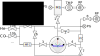
\includegraphics[width=0.75\textwidth]{02_Tools/fig/setup_Fuzhou.png}
	\caption{Valve diagram of EC-MS setup at Fuzhou. In reality, at the time of writing this thesis, the pressure controller is actually a modified pressure regulator, which works but is not as stable.}
	\label{fig:Fuzhou}
\end{figure}

The sniffer setup described above can be considered a ``delux setup'' with an excess of components to maximize functionality. The group in Fuzhou asked me to design a ``budget setup'' which captured the central advantages of chip EC-MS with as few components as possible. They then built my design, shown in Figure \ref{fig:Fuzhou} with the outside help from a Chinese mass spectrometer company, Quantang Instruments. Much to my frustruation, Quantang built a box around the valve system, making it quite tedious to make changes to the system, and put their logo and the name ECMS200A on the box.

All of the concepts are the same as for the sniffer setup, but the operation is different. The procedures for chip pump-down and carrier gas exchange are described in Appendix \ref{app:Fuzhou}. The cost of having one less Turbo pump is the need to wait for long pumping periods and to turn off the filament of the mass spectrometer when changing chips. The carrier gas exchange procedure is actually slightly simpler than that of the sniffer setup and saves three MFC's and a PC. The only disadvantage is that, with only one MFC, it is not easy to prepare a controlled gas mixture (a functionality I have rarely used on the sniffer setup).

\subsection{Changing chip}
The procedure to change chip is as follows:
\begin{enumerate}
	\item Isolate the chip: Close Valves 1, 2, 3, and 4. Double-check that Valve 1 is closed!!! Also, turn off the filament of the mass spectrometer
	
	\item Remove the old chip and install the new one.
	
	\item Open valve 2 (Valve 8 is normally always open). This removes air from the post-capillary volume through the roughing pump.
	
	\item Wait until the pressure is less than 0.01 mbar (1 Pa, the unit on the Chinese displays). This takes approximately half an hour.
	
	\item Double check that the filament of the mass spectrometer is turned off, as the roughing pressure could damage it. Then open Valve 1. 
	
	\item Immediately close Valve 2.
	
	\item When the pressure in the mass spectrometer is less than $10^{-5}$ mbar ($10^{-3}$ Pa), turn on the filament again. After this, it will take a couple hours before the MS signals are stable.	
\end{enumerate}



\subsection{Changing carrier gas}
The procedure for changing carrier gases (with He to CO as an example) is as follows:
\begin{enumerate}
	\item At first, He is flowing through Valve 10a, the MFC (set to 1 ml/min), Valve 3, the chip, Valve 4, the pressure controller set to 1 bar (actually a pressure regulator, adjusted to maintain 0 vs atmosphere), Valve 8 and the RP. 
	
	\item Close Valves 3 and 4. The electrochemistry experiment can then continue in He while getting the new carrier gas ready.
	
	\item Close Valve 10a and set the MFC to zero.
	
	\item Pump out the He. This involves opening Valves 5, 6, and 7, and setting PC to zero.
	
	\item Close Valves 5 and 6 and set PC to 1 bar.
	
	\item Fill up CO: Open Valve 10b. Then set the MFC to 10 ml/min. flow until the pressure read at PC is 1 bar.
	
	\item Close Valve 7 and open Valves 3 and 4. The carrier gas change should immediately be visible 
	
	\item Set the CO flow to 1 ml/min. The setup is now in steady operation in CO carrier gas.
\end{enumerate}



\section{Spectro Inlets}\label{app:spectro}

\begin{figure}[h!]
	\centering
	\includegraphics[width=0.75\textwidth]{02_Tools/fig/spectro.png}
	\caption{Photos of the setup at Spectro Inlets ApS. From their website: \url{https://spectroinlets.com/}}
	\label{fig:spectro}
\end{figure}
Finally, I should mention that there is now a commercially available setup which combines the best of both worlds: The functionality of the Sniffer setup and the simplicity and compactness of the ECMS200A. This is made possible in part due to some custom vacuum components. The setup, sold by Spectro Inlets ApS, is shown in the photographs in Figure \ref{fig:spectro}. I have been involved in conversations aiding the development of this setup, as a kind of test user, but can't go to detail here on its design. The Spectro Inlets setup also comes with a software automating the chip pump-down and carrier gas exchange procedures. The procedures described in Appendix \ref{app:instructions} for the other two setups are thus simplified to pressing a button.



\section{Sputtering \ch{Ru^{18}O2} and \ch{Ir^{18}O2}}\label{app:sputter}

This appendix serves as the sample prep methods for most of Chapter \ref{ch:O2}, as well as instructions for sputter deposition using \ch{^{18}O2}.

\subsection{Switching \ch{O2} source}
First, prepare the reactant gas. This requires a pump-down step to avoid mixing the natural \ch{O2} and the 99\% \ch{^{18}O2}.
\begin{enumerate}
	\item Make sure the flow is off (AJA software) and the reactant gas valve on the top of the sputter chamber (manually controlled) is open!
	
	\item Make sure both the natural oxygen (\ch{^{16}O2}) and \ch{^{18}O2} valves nearest the switch (the T intersection just before the flow controller) are closed.
	
	\item Evacuate the switch through the sputter chamber. This is a bit tedious because the AJA software will try to close the pneumatic valve when the flow doesn't reach set point. First flow at 10 ml/min until there is so little gas that this flow rate cannot be met. Then set it to 0.5 ml/min and leave it for an hour. The AJA software seems to have a tolerance of 0.5 ml/min before automatically closing the valves, so this will leave it open.
	
	\item Turn off the flow with the AJA software.
	
	\item Open the valve connecting the desired \ch{O2} source to the switch. 
	
	\item If you are using \ch{^{18}O2}, briefly open the valve on the bottle and close it again. The \ch{^{18}O2} in the line should then be enough for depositing a film, and this will avoid making a mistake that would waste the remaining gas.
\end{enumerate}

\subsection{Deposition}
The sputter deposition  process for nominally 25 (10) nm of \ch{Ru^{18}O2} (\ch{Ir^{18}O2}) is as follows:
\begin{enumerate}
	\item Load the samples via the load lock, and heat the samples to the desired temperature. 400$^\circ$C gives crystalline, rutile films.
	
	\item Pre-clean the chamber with an argon plasma for 5 minutes. Use 20 ml/min Ar, 20 mTorr, and 35 Watts.
	
	\item Put the screen in front of the samples. Sputter titanium. Use 20 ml/min Ar, 3 mTorr, and 160 W. You may need to start the plasma at 10 mTorr and then ramp down. This step is to remove any residual oxygen in the chamber to achieve isotopic purity. (This step can be skipped when not doing isotope-labeled films.)
	
	\item After titanium has been sputtering for 15 minutes, remove the screen and allow it to keep sputtering, now onto the samples, for another three minutes. This establishes a $\approx$ 5 nm thick Ti sticking layer. After three minutes, close the shutter again and keep sputtering Ti for another three minutes before turning off the Ti plasma.
	
	\item Increase the pressure to 5 mTorr and lower the Ar flow rate to 5 ml/min. 
	
	\item Start the plasma on the Ru (Ir) target. Use 60 W (30 W).
	
	\item Start the \ch{^{18}O2} flow at 1 ml/min.
	
	\item Open the shutter to the Ru (Ir) target. 
	
	\item Time 1500 s (700 s), and then close the shutter
	
	\item Turn off the plasma.
	
	\item Turn off the gas flows.
	
	\item Let the samples cool before taking them out through the load lock.
\end{enumerate}


\section{ICP-MS}\label{app:sampling}


Briefly, the electrolyte in the cell is sucked out with a syringe while new electrolyte flows in from an electrolyte delivery tower. The old electrolyte stored in an Eppendorf tube and the syringe is re-inserted. This results in electrolyte samples of $\approx 0.5$ ml in Eppendorf tubes. 

For study with ICP-MS, the raw samples are first diluted to a standard volume of 1 ml with 2\% \ch{HNO3}, 0.1 ml of this is then diluted to 10 ml with 2\% \ch{HNO3}, which is the ICP-MS sample. The concentration of this ICP-MS sample is then as if all of the metal dissolved during the experiment were diluted in 100 ml. The amount of metal $n^i$ (typically stated in pmol) can then be determined from its mass concentration $c_m^i$ in the ICP-MS sample (typically stated in $\mu$g per l which is numerically equivalent to ppb) by
\begin{equation}
n^i = 100\,\text{[ml]}\frac{c_m^i}{M^i}\,,\label{eq:ppb_to_pmol}
\end{equation}
where $M^i$ is the molar mass of $i$.

To determine $c_m^i$ from the raw signal (in counts) requires calibration. A dilution series (typically 0.1, 1, 10, and 100 $\mu$g/l) is prepared from a standard stock solution. These are measured together with the samples and intervening measurements a blank solution (2\% \ch{HNO3} in water with no metals). The calibration curve is made by drawing a line of best fit through the counts vs concentrations of this dilution series on a log-log plot (the slope of this line should be 1). Typical calibration curves for Ir and Ru are shown in Figure \ref{fig:ICPMS_cal}. These calibration curves are made using the function \texttt{ICPMS\_calibration} of the \texttt{EC\_MS} python package (see Appendix \ref{app:EC_MS}).

\begin{figure}[h!]
	\centering
	\includegraphics[width=\textwidth]{02_Tools/fig/ICPMS_calibration_curves.png}
	\caption{Calibration curves for ICP-MS detection of \textbf{(a)} Ir and \textbf{(b)} Ru. The top x-axes represents the amount of metal originally in a sample from the EC-MS setup, and is scaled to the bottom x-axis according to Equation \ref{eq:ppb_to_pmol}. The dashed black line is the mean number of counts in blank measurements, and the dotted black line is that mean plus three times the standard deviation of the number of counts in the blank measurement. The detection limit, defined as where the latter intercepts the calibration curve, is indicated with a green vertical line.}
	\label{fig:ICPMS_cal}
\end{figure}

The detection limit is defined as the amount corresponding to the counts of the blank measurements plus three times the standard deviation of counts the blank measurements\cite{Harris2010}. This is 1.4 pmol for Ir and 3.1 pmol for Ru.


\subsection{Electrolyte sampling}
It is possible with the sniffer setup to take electrolyte samples out under potential control for analysis with ICP-MS. This requires an electrolyte delivery bottle on one side and a syringe on the other side, as shown in Figure \ref{fig:ICPMS} on Page \pageref{fig:ICPMS}. To set this up (items 1 through 4 are the standard procedure):
\begin{enumerate}
	\item Align the sample in the cell
	
	\item Mount the cell on the interface block
	
	\item Fill the cell with electrolyte using the syringe
	
	\item Insert the RE and CE glassware when the electrolyte forms a miniscus in the Luer fitting
	
	\item When there is a miniscus of electrolyte coming out of the outlet (male Luer fitting), very quickly open the valve on the electrolyte delivery tower and push the tube onto the Luer fitting, connecting the tower and the cell. This should be done quickly to minimize spilling. Clean up any spill right a way with a paper wipe.
	
	\item Close the valve.
\end{enumerate}

It is important that valve is open while the electrolyte delivery tower is connected the cell to avoid developing an overpressure which could breach the chip. It is good for it to be closed during the experiment, or the pressure of the electrolyte above the valve can push electrolyte into the cell and exascerbate any leaks that might be present.

To take an electrolyte sample:
\begin{enumerate}
	\item Open the valve to the electrolyte delivery tower
	
	\item Pull 0.5 ml of electrolyte with the syringe. Do so as steadily as possible to avoid making an underpressure which could pull carrier gas from the chip into the working volume. Bubbles are the enemy!
	
	\item Remove the syringe and close the valve of the electrolyte delivery tower as fast as possible to minimize spillage. Clean up any spillage.
	
	\item Empty the syringe into an eppendorf tube or other storage. This is your sample for ICP-MS.
	
	\item Very quickly open the valve to the electrolyte delivery tower and quickly re-insert the syringe.
	
	\item Close the valve. You're ready to take the next sample when the time comes.
\end{enumerate}


	
	%\chapter{Papers from this PhD Project}
		
		\renewcommand{\thesection}{\Roman{section}}
		\titleformat{\section}{\normalfont\Large\bfseries}{Paper~\thesection}{1em}{}	
		
		\section{Enabling real-time detection of electrochemical desorption phenomena with sub-monolayer sensitivity}\label{Trimarco2018}
		
		Daniel B. Trimarco*, Soren B. Scott*, Anil H. Thilsted, Jesper Y. Pan, Thomas Pedersen, Ole Hansen, Ib Chorkendorff, and Peter C.K. Vesborg. 
		
		*These authors contributed equally to this work
		
		\textit{Electrochimica Acta}, 2018, 268, 520-530
		
		DOI: 10.1016/j.electacta.2018.02.060
		
		\includepdf[pages=-]{Appendices/articles/Trimarco2018.pdf}
		
		
		
		
		\clearpage
		\section{Impact of nanoparticle size and lattice oxygen on water oxidation on \ch{NiFeO$_x$H$_y$}}\label{Roy2018}
		
		Claudie Roy*, Bela Sebok*, Soren B. Scott*, Elisabetta M. Fiordaliso, Jakob E. Sørensen, Anders Bodin, Daniel B. Trimarco, Christian D. Damsgaard, Peter C. K. Vesborg, Ole Hansen, Ifan E. L. Stephens, Jakob Kibsgaard and Ib Chorkendorff. 
		
		*These authors contributed equally to this work
		
		\textit{Nature Catalysis}, 2018, 1(11), 820-829 
		
		DOI: 10.1038/s41929-018-0162-x
		
		\includepdf[pages=-]{Appendices/articles/Roy2018.pdf}	
		
		
		
		
		
		\clearpage
		\section{Towards an Atomistic Understanding of Electrocatalytic Partial Hydrocarbon Oxidation: Propene on Palladium}\label{Winiwarter2019}
		
		Anna Winiwarter*, Luca Silva*, Soren B. Scott, Kasper Enemark-Rasmussen, Manuel Saric, Daniel B. Trimarco, Peter C. K. Vesborg, Poul G. Moses, Ifan E. L. Stephens, Brian Seger, Jan Rossmeisl, and Ib Chorkendorff.
		
		*These authors contributed equally to this work
		
		\textit{Energy and Environmental Science}, 12, 1055-1067, 2019.
		
		DOI:  10.1039/C8EE03426E
		
		\includepdf[pages=-]{Appendices/articles/Winiwarter2019.pdf}
		
		
		
		
		\clearpage
		\section{Absence of Oxidized Phases in Cu under CO Reduction Conditions}\label{Scott2019_GIXRD}
		
		Soren B. Scott, Thomas V. Hogg, Alan T. Landers, Thomas Maagaard, Erlend Bertheussen, John C. Lin, Ryan C. Davis, Jefferey W. Beeman, Drew Higgins, Walter S. Drisdell, Apurva Mehta, Brian J. Seger, Thomas F. Jaramillo, and Ib Chorkendorff.
		
		\textit{ACS Energy Letters}. 4, 803−804, 2019
		
		DOI: 10.1021/acsenergylett.9b00172 
		
		\includepdf[pages=-]{Appendices/articles/Scott2019.pdf}





		\clearpage
		\section{Progress and Perspectives of Electrochemical CO2 Reduction on Copper in Aqueous Electrolyte}\label{Nitopi2019}
		
		Stephanie A. Nitopi*, Erlend Bertheussen*, Soren Bertelsen Scott, Xinyan Liu, Albert K. Engstfeld, Sebastian Horch, Brian Seger, Ifan Stephens, Karen Chan, Christopher Hahn, Jens K. Nørskov, Thomas Jaramillo, and Ib Chorkendorff.
		
		*These authors contributed equally to this work
		
		\textit{Chemical Reviews}. 12, 7610-7672, 2019
		
		DOI: 10.1021/acs.chemrev.8b00705
		
		\vspace{2cm}
		
		\textbf{Note:}
		
		I became involved in this Paper, a review and perspective article, because I wrote a motivation for the \ch{CO2} reduction reaction as part of my master's thesis, which I expanded and adapted for this Paper. My primary contributions to the Paper were writing the introduction and producing a map of proposed mechanistic pathways of \ch{CO2} reduction. The Paper is 63 pages long, and so only the introduction is reproduced in this thesis.	
		
		
		\includepdf[pages=1-8]{Appendices/articles/Nitopi2019_ChemRev.pdf}
		\clearpage
		\vspace{5cm}
		
		%\includepdf[pages=27]{Appendices/articles/Nitopi2019_ChemRev.pdf}
		
		{
			\hspace{0pt}
			\vfill
			Stephanie A. Nitopi, Erlend Bertheussen, Soren Bertelsen Scott, Xinyan Liu, Albert K. Engstfeld, Sebastian Horch, Brian Seger, Ifan Stephens, Karen Chan, Christopher Hahn, Jens K. Nørskov, Thomas Jaramillo, and Ib Chorkendorff. Progress and Perspectives of Electrochemical CO2 Reduction on Copper in Aqueous Electrolyte. \textit{Chemical Reviews}. XXXX, XXX, XXX-XXX, 2019
			
			\vspace{1cm}
			
			\centering\Large
			Pages I-AX and BC - BK of this publication are not included in this thesis
			\vfill
			\hspace{0pt}
		}
		\clearpage
		
		\includepdf[pages=51-54]{Appendices/articles/Nitopi2019_ChemRev.pdf}
		


	
		\clearpage
		\section[In Preparation - Desorbing uphill: Anodic Hydrogen Evolution on Cu and Ru Electrodes]{Desorbing uphill: Anodic Hydrogen Evolution on Cu and Ru Electrodes}\label{Scott_Engstfeld2019}
		
		Søren B. Scott*, Albert K. Engstfeld*, Zenonas Yusys, Degenhart Hochfilzer, Nikolaj Knøsgaard, Daniel B. Trimarco, Peter C.K. Vesborg, R. Jürgen Behm, and Ib Chorkendorff
		
		\textit{In preparation}
		
		\includepdf[pages=-]{Appendices/articles/Scott_Engstfeld2019.pdf}
		
		
		
				
		\clearpage
		\section[In Preparation - Mechanistic study of oxygen evolution on \ch{RuO2} down to 60 mV overpotential]{Mechanistic study of oxygen evolution on \ch{RuO2} down to 60 mV overpotential}\label{Scott_Rao2019}
		
		\underline{Soren B. Scott}*, Reshma R. Rao*, Choongman M. Moon, Jakob E. S\o rensen, Jakob Kibsgaard, Yang Shao-Horn, and Ib Chorkendorff
		
		*These authors contributed equally to this work
		
		\textit{In Preparation}
	
	
	

	
	\chapter{Python Packages Developed During this PhD Project}
		\section{\texttt{EC\_MS} and \texttt{EC\_Xray}}
%\end{appendices}\clearpage

\end{document}
